%!Mode:: "TeX:UTF-8"
%!TEX program=xelatex
%!TEX TS-program=xelatex
%!TEX encoding=UTF-8 Unicode
\RequirePackage{fix-cm}%优化字体
\documentclass[UTF8,aspectratio=43,11pt,colorlinks,compress,openany]{beamer}%aspectratio=169%169宽屏 43窄屏[handout]

\input{preamble-beamer}
\input{beamer-light}%monokai,dark,light


\begin{document}
%%%%%%%%%%%%%%%%%%%%%%%%%%%%
\title{Elementary Logic}
\author{
	{\includegraphics[width=0.1\textwidth,angle=0,origin=c]{img/lixi.pdf}}\\
	\small Department of Philosophy\\
	\footnotesize Central South University\\
	\scriptsize xieshenlixi@163.com\\
	\scriptsize \href{https://github.com/rickylixi/logic}{github}
}
\date{\today}
\maketitle
%%%%%%%%%%%% 节前目录 %%%%%%%%%%
\AtBeginSection[]
{
\frame[shrink]{{Contents}
\begin{multicols}{2}
\tableofcontents[currentsection,hideallsubsections]
\end{multicols}
}
\addtocounter{framenumber}{-1} %目录页不计页码
}
\AtBeginSubsection[]
{
\frame[shrink]{{Contents}
\begin{multicols}{2}
\tableofcontents[sectionstyle=show/shaded,subsectionstyle=show/shaded/hide,subsubsectionstyle=hide]
\end{multicols}
}
\addtocounter{framenumber}{-1} %目录页不计页码
}





%%%%%%%%%%%%%%%%%%%%%%%%%%%%
\section{Introduction}
%%%%%%%%%%%%%%%%%%%%%%%%%%%%

%%%%%%%%%%%%%%%%%%%%%%%%%%%
\subsection{Logic Puzzle}
%%%%%%%%%%%%%%%%%%%%%%%%%%%

\begin{frame}\frametitle{Information Update}
\begin{block}{Five Logicians Walk into a Bar}
	\begin{itemize}
		\item \textbf{Waiter:} Do you all want beer?
		\item \textbf{1:} I don't know.
		\item \textbf{2:} I don't know.
		\item \textbf{3:} I don't know.
		\item \textbf{4:} I don't know.
		\item \textbf{5:} No.
	\end{itemize}	
\end{block}
The information content of a formula $A$ is the set $\operatorname{Mod}(A)$ of its models. An update with new information $B$ reduces the current set of models $\operatorname{Mod}(A)$ to the overlap of $\operatorname{Mod}(A)$ and $\operatorname{Mod}(B)$.
\end{frame}

\begin{frame}\frametitle{Unfaithful Husband Puzzle}
	\begin{problem}[Unfaithful Husband Puzzle]
		\begin{enumerate}
			\item Every man in a village of $100$ married couples has cheated on his wife.
			\item Every wife in the village knows about the fidelity of every man in the village except for her own husband.
			\item One day, the queen visits and announces that at least one husband has been unfaithful, and that any wife who discovers his husband's infidelity must kill him that very day.
			\item What happens?
		\end{enumerate}
	\end{problem}\vspace{-2ex}
\begin{columns}
\column{.35\textwidth}
	\begin{figure}
	\includegraphics[width=\textwidth]{img/emperor}
	\end{figure}
\column{.47\textwidth}
	After a date, one says to the other:\\
	\textcolor{red}{``Would you like to come up to my apartment to see my etchings?''}
\end{columns}
\end{frame}

\begin{frame}\frametitle{}
\begin{block}{Test}
Guess what $2/3$ of the average of your guesses will be, where the numbers are restricted to the real numbers between $0$ and $100$.
\end{block}
\end{frame}

\begin{frame}\frametitle{}
\begin{problem}
周迅的前男友窦鹏是窦唯的堂弟;窦唯是王菲的前老公;周迅的前男友宋宁是高原的表弟;高原是窦唯的前任老婆;周迅的前男友李亚鹏是王菲的现任老公;周迅的前男友朴树的音乐制作人是张亚东;张亚东是王菲的前老公窦唯的妹妹窦颖的前老公,也是王菲的音乐制作人;张亚东是李亚鹏前女友瞿颖的现男友。\\
下列说法不正确的是:
\begin{enumerate}
\item 王菲周迅是情敌关系
\item 瞿颖王菲是情敌关系
\item 窦颖周迅是情敌关系
\item 瞿颖周迅是情敌关系
\end{enumerate}
\end{problem}
\end{frame}

\begin{frame}[fragile]\frametitle{Gateway to Heaven}
	\begin{problem}[\switchocg{ocg1}{天堂之路}]
		\begin{itemize}
			\item 你面前有左右两人守卫左右两门。
			\item 一人只说真话,一人只说假话。
			\item 一门通天堂,一门通地狱。
			\item 你只能向其中一人提一个“是/否”的问题。
			\item 怎么问出去天堂的路?
		\end{itemize}
	\end{problem}
\begin{ocg}{heaven-hell}{ocg1}{0}
\begin{verbatim}
你说真话且左门通天堂,或者,你说假话且右门通天堂,是吗?
如果我明天问你,左门通天堂吗?你会说“是”吗?
如果我问另一个人,左门通天堂吗?他会说“是”吗?
\end{verbatim}
\end{ocg}
\end{frame}

\begin{frame}\frametitle{\href{https://mp.weixin.qq.com/s/CEtNyU3OMChVg5vMX5fnLA}{Hardest Logic Puzzle Ever}}
	\begin{problem}[Hardest Logic Puzzle Ever]
		\begin{itemize}
			\item Three gods, $A$, $B$, and $C$ are called in some order, $T$, $F$, and $R$.
			\item $T$ always speaks truly, $F$ always speaks falsely \textcolor{yellow}{(if he is certain he can; but if he is unable to lie with certainty, he responds like $R$)}, but whether $R$ speaks truly or falsely \textcolor{yellow}{(or whether $R$ speaks at all)} is completely random.
			\item Your task is to determine the identities of $A$, $B$, and $C$ by asking $2$ \textcolor{yellow}{($3$)} yes/no questions; each question must be put to exactly one god.
			\item The gods understand English, but will answer in their own language, in which the words for `yes' and `no' are `da' and `ja' in some order. You don't know which word means which.
		\end{itemize}
	\end{problem}
\end{frame}


%%%%%%%%%%%%%%%%%%%%%%%%%%%%%%%
\subsection{Textbook and Homework}
%%%%%%%%%%%%%%%%%%%%%%%%%%%%%%%

\begin{frame}\frametitle{Outline}
	\begin{itemize}
		\item Critical Thinking \textcolor{red}{$\checkmark$}
		\item History
		\item Term Logic
		\item Propositional Logic \textcolor{red}{$\checkmark$}
		\item Predicate Logic \textcolor{red}{$\checkmark$}
		\item Equational Logic
		\item Set Theory
		\item Recursion Theory
		\item Modal Logic
	\end{itemize}
\end{frame}

\begin{frame}\frametitle{Readings}
		\begin{enumerate}
			\item P.~J.~Hurley: A Concise Introduction to Logic.\hfill --- $B$
			\item H.~de~Swart: Pilosophical and Mathematical Logic.\hfill --- $P$
			\item P.~Smith: An Introduction to Formal Logic.\hfill --- $P$
			\item \href{http://www.logicmatters.net/tyl}{\emph{P.~Smith: Teach Yourself Logic.}\hfill --- $P$}
			\item \href{http://www.logicinaction.org}{J.~van Benthem: Logic in Action.\hfill --- $P$}
			\item \href{http://builds.openlogicproject.org}{Open Logic Project.\hfill --- $P$}
			\item \textcolor{yellow}{H.~Enderton: A Mathematical Introduction to Logic.\hfill --- $\textbf{L}$}
			\item H.~Ebbinghaus, J.~Flum, W.~Thomas: Mathematical Logic.\hfill --- $L$
			\item A.~Nerode, R.~A.~Shore: Logic for Applications.\hfill --- $\textcolor{green}{C}$
			\item Yuri Manin: A Course in Mathematical Logic for Mathematicians.\hfill --- $\textcolor{green}{M}$
		\end{enumerate}
\end{frame}

\begin{frame}\frametitle{Readings, Movies and More}
	\begin{columns}
		\column{.55\textwidth}
		\begin{figure}[H]
			\subfigure{\includegraphics[height=.33\textheight]{img/ml-chen.jpg}}
			\subfigure{\includegraphics[height=.33\textheight]{img/ml-yang}}
			\subfigure{\includegraphics[height=.33\textheight]{img/geb.jpg}}
		\end{figure}
\column{.35\textwidth}
\begin{block}{Hofstadter's Law}
It always takes longer than you expect, even when you take into account Hofstadter's Law.
\end{block}
	\end{columns}
\begin{columns}
		\column{.56\textwidth}
			\begin{itemize}
				\item \textcolor{green}{D.~Hofstadter: G\"odel, Escher, Bach}
				\item \textcolor{yellow}{Dangerous Knowledge}
				\item The Imitation Game
			\end{itemize}
			\begin{itemize}
				\item Philosophical Logic
				\item Philosophy of Logic
				\item Philosophy of Mathematics
			\end{itemize}
\column{.27\textwidth}
		\begin{block}{}
			\begin{itemize}
				\item \href{https://en.wikipedia.org/wiki/Library_Genesis}{libgen}
				\item \href{https://en.wikipedia.org/wiki/Sci-Hub}{sci-hub}
				\item \href{https://github.com/XX-net/XX-Net}{XX-Net}
				\item \href{http://googlehelper.net/}{ghelper}
				\item Google Cloud
				\item JJQQKK
			\end{itemize}
		\end{block}
\end{columns}
\end{frame}

\begin{frame}\frametitle{Exams and Credits}
	\begin{itemize}
		\item Question
		\item Discussion
		\item \textcolor{red}{Exercises/Homework} $\checkmark$
		\item Presentation
		\item Paper
		\item \textcolor{red}{Examination} $\checkmark$
		\item Techniques e.g. \LaTeX\, / Coq \dots
		\item \dots
	\end{itemize}
\end{frame}

\begin{frame}\frametitle{Homework}
		\href{https://www.google.com/}{Google}/\href{https://www.wikipedia.org/}{Wikipedia}/\href{https://plato.stanford.edu/}{Stanford Encyclopedia}/\href{https://www.iep.utm.edu/}{Internet Encyclopedia}
		\begin{itemize}
			\item Leibniz, Cantor, Frege, Russell, Hilbert, G\"odel, Tarski, Turing.
			\item finite, infinite, syntax, semantics, formal system, deduction, logical consequence, consistency, satisfiability, validity, soundness, completeness, compactness, decidability
			\item Philosophy of Logic, Philosophical Logic
			\item Logicism, Formalism, Intuitionism
			\item Hilbert's program
			\item Church-Turing thesis
		\end{itemize}
\end{frame}

\begin{frame}\frametitle{Aim}
	\begin{itemize}
		\item Critical thinking \textcolor{red}{$\checkmark$}
		\item Formalization of an argument \textcolor{red}{$\checkmark$}
		\item Demonstration of the validity of an argument \textcolor{red}{$\checkmark$}
		\item {\small Object \& Meta-language / Syntax \& Semantics / Finite \& Infinite / Countable \& Uncountable / Induction \& Recursion / Truth \& Proof / Axiomatization / Theory / Soundness / Completeness / Compactness / Elementary Equivalent \& Isomorphism / Representability / Definability / Categoricity / Decidability / Complexity / Expressiveness / Succinctness / Interpretability \dots} \textcolor{green}{$\surd$}
		\item \href{https://plato.stanford.edu/entries/formal-epistemology/}{Formal Philosophy}
		\item Understanding of the nature of mathematics
		\item Application in Math / CS / AI / Linguistics / Cognition / Physics / Information Theory / Game Theory / Social Science \dots
		\item Mathematical Logic
	\end{itemize}
\end{frame}

\begin{frame}\frametitle{The Music of Reason}
	\begin{center}
		\large{\textcolor{yellow}{\textbf{How to \textit{express} your thoughts \underline{precisely} and \underline{succinctly}?}}}
	\end{center}
	\begin{figure}
		\includegraphics[width=0.9\textwidth]{img/music.png}
	\end{figure}
	\begin{center}
	The glory of the human spirit!\\
	\large{\textcolor{red}{What are the extent and limits of reason?}}
	\end{center}
\end{frame}

%%%%%%%%%%%%%%%%%%%%%%%%%%%%%
\subsection{Logic and other Disciplines}
%%%%%%%%%%%%%%%%%%%%%%%%%%%%%

\begin{frame}\frametitle{Logic vs other Disciplines}
		\begin{itemize}
			\item Logic vs (Analytic) Philosophy.
			
			sense \& reference / extension \& intension / use \& mention / truth \& provability / mutual vs distributed vs common knowledge / knowledge update / belief revision / preference change / information flow / action \& strategy / multi-agent interaction / counterfactual / causation / possible world / cross-world identity / essentialism / induction / ontological commitment / concept analysis / laws of thought / strength \& limitation / paradoxes \dots
			
			Peirce, Frege, Russell, Wittgenstein, Ramsey, Carnap, Quine, Putnam, Kripke, Chomsky, G\"odel, Tarski, Turing \dots
			\item Logic vs Mathematics.
			
			Logicism / Formalism / Intuitionism / Constructivism / Finitism / Structuralism / \href{https://homotopytypetheory.org/book/}{Homotopy Type Theory}
			\item Logic vs Computer Science.
			\[\dfrac{\text{Logic}}{\text{Computer Science}} \approx \dfrac{\text{Calculus}}{\text{Physics}}\]
		\end{itemize}
\end{frame}

\begin{frame}[shrink]\frametitle{Branches of Logic}
\vspace*{-1ex}
	\resizebox{\textwidth}{!}{
		\begin{minipage}{1.1\textwidth}
			\begin{columns}
				\column{0.33\textwidth}
				\begin{itemize}
					\item[] \textbf{\hspace*{-18pt} Mathematical Logic}
				\end{itemize}
				\column{0.35\textwidth}
				\begin{itemize}
					\item[] \textbf{\hspace*{-20pt} Computational Logic}
				\end{itemize}
				\column{0.32\textwidth}
				\begin{itemize}
					\item[] \textbf{\hspace*{-8pt} Philosophical Logic}
				\end{itemize}
			\end{columns}\vspace*{-1ex}
			\begin{columns}
				\column{0.34\textwidth}
					\begin{itemize}
						\item \textbf{\textcolor{yellow}{First Order Logic}}
						\item \textcolor{green}{Set Theory}
						\item \textcolor{green}{Model Theory}
						\item \textcolor{green}{Proof Theory}
						\item \textcolor{green}{Recursion Theory}
					\end{itemize}
				\column{0.39\textwidth}
					\begin{itemize}
						\item Automata Theory
						\item Computational Complexity
						\item Finite Model Theory
						\item Model Checking
						\item Type Theory
						\item Lambda Calculus
						\item Categorical Logic
						\item Theorem Proving
						\item Description Logic
						\item Dynamic Logic
						\item Temporal Logic
						\item Hoare Logic
						\item Inductive Logic
						\item Fuzzy Logic
						\item Non-monotonic Logic
						\item Computability Logic
						\item Default Logic
						\item Situation Calculus
					\end{itemize}
				\column{0.34\textwidth}
					\begin{itemize}
						\item Intuitionistic Logic
						\item Algebraic Logic
						\item Quantum Logic
						\item \textcolor{red}{Modal Logic}
						\item Epistemic Logic
						\item Doxastic Logic
						\item Preference Logic
						\item Provability Logic
						\item Hybrid Logic
						\item Free Logic
						\item Conditional Logic
						\item Relevance Logic
						\item Linear Logic
						\item Paraconsistent Logic
						\item Intensional Logic
						\item Partial Logic
						\item Diagrammatic Logic
						\item Deontic Logic
					\end{itemize}
			\end{columns}
	\end{minipage}}
\end{frame}

\begin{frame}\frametitle{$\nabla(\odot\!\cdot\!\odot)=\operatorname{\odot\nabla\odot}+\operatorname{\odot\nabla\odot}$}
\begin{columns}
\column{.65\textwidth}
	\Large{
		\begin{itemize}
			\item Logic is
			\begin{enumerate}
				\item mainly philosophy by subject matter
				\item mainly mathematics by methodology
				\item mainly computer science by applications
			\end{enumerate}
			\item Logicians always want to be
			\begin{enumerate}
				\item Philosophers of philosophers
				\item Mathematicians of mathematicians
				\item Computer scientists of computer scientists
			\end{enumerate}
			\item However, they often end up being
			\begin{enumerate}
				\item Mathematicians to philosophers
				\item Computer scientists to mathematicians
				\item Philosophers to computer scientists
			\end{enumerate}
	\end{itemize}}
\column{.45\textwidth}
					\begin{tikzpicture}[scale=0.43]
					\draw[very thick](6,2.5)circle(3 and 3)node(C){${\textbf{CS}}\atop{\textit{useful}}$};
					\draw[very thick](8,6)circle(3 and 3)node(P){${\textbf{Philo}}\atop{\textit{to the point}}$};
					\draw[very thick](10,2.5)circle(3 and 3)node(M){${\textbf{Math}}\atop{\textit{rigid}}$};
					\begin{scope}
					\clip(8,6)circle(3 and 3);
					\clip(10,2.5)circle(3 and 3);
					\clip(6,2.5)circle(3 and 3);
					\filldraw[fill=gray,nearly transparent,opacity=.5](0,0)rectangle(10,5);
					\end{scope}
					\node at ($0.33*(C)+0.33*(M)+0.33*(P)$){$\textcolor{red}{\textbf{L}}$};
					\end{tikzpicture}
\end{columns}
\end{frame}


%%%%%%%%%%%%%%%%%%%%%%%%%%%%%%%%
\section{History}
%%%%%%%%%%%%%%%%%%%%%%%%%%%%%%%%


%--------------------------------%
\subsection{The Prehistory of Logic}
%--------------------------------%

\begin{frame}\frametitle{Aristotle(384-322 BC) --- Term Logic}
	\begin{columns}
		\column{0.7\textwidth}
			\begin{itemize}
				\item Three Modes of Persuasion in Rhetoric: Ethos, Pathos, and Logos.
				\item Term Logic.
				\item Aristotle believed that any logical argument can, in principle, be broken down into a series of applications of a small number of syllogisms.
				\item Four Causes: material/formal/efficient/final
			\end{itemize}
		\column{0.2\textwidth}
			\begin{figure}
				\includegraphics[width=\textwidth]{img/aristotle.jpg}
			\end{figure}
	\end{columns}
\end{frame}

\begin{frame}\frametitle{Leibniz 1646-1716}
	\begin{columns}
		\column{0.57\textwidth}
			\begin{block}{}
				\centerline{\Large Don't argue. Calculate!}
			\end{block}
			\begin{itemize}
				\item \textcolor{green}{{\small Principle of Contradiction}}: Nothing can be and not be, but everything either is or is not.
				\item \textcolor{green}{{\small Principle of Sufficient Reason}}: Nothing is without a reason.
				\item \textcolor{yellow}{{\small Principle of Perfection}}: The real world is the best of all possible worlds.
			\end{itemize}
			\begin{block}{In the beginning was the Logic.}
				As God calculates, so the world is made.
			\end{block}
		\column{0.23\textwidth}
			\begin{figure}
				\includegraphics[width=\textwidth,angle=0,origin=c]{img/leibniz0.jpg}
			\end{figure}
	\end{columns}
\end{frame}

\begin{frame}\frametitle{Leibniz's Dream --- Deduction}
		\begin{enumerate}[1]
			\item Characteristica Universalis \& Calculus Ratiocinator.
			\begin{enumerate}[i]
				\item \textcolor{green}{the coordination of knowledge in an encyclopedia} --- collect all present knowledge so we could sift through it for what is fundamental. With the set of ideas that it generated, we could formulate the \emph{characteristica universalis}. (which form the alphabet of human thought).
				\item \emph{\textbf{characteristica universalis}} --- a \textcolor{green}{universal ideal language} whose rules of composition directly expresses the structure of the world.
					\[\textcolor{yellow}{\text{sign}\rightleftarrows\text{idea}}\]
					\begin{center}
						{\footnotesize \textcolor{yellow}{
								encyclopedia $\Rightarrow$ fundamental principles $\Rightarrow$ primitive notions}}
					\end{center}
				\item \emph{\textbf{calculus ratiocinator}} --- the arrangement of \textcolor{green}{all true propositions} in an \textcolor{green}{axiomatic system}.
				\item \textcolor{green}{decision procedure}. --- an algorithm which, when applied to any formula of the \emph{characteristica universalis}, would determine whether or not that formula were true. \textcolor{red}{--- a procedure for the rapid enlargement of knowledge. replace reasoning by computation. the art of invention. free mind from intuition.}
				\item a proof that the \emph{calculus ratiocinator} is \textcolor{green}{consistent}.
			\end{enumerate}
		\end{enumerate}
\end{frame}

\begin{frame}\frametitle{\href{https://philpapers.org/rec/HACTLP}{Leibniz's Dream --- Induction}}
		\begin{figure}
			\includegraphics[width=0.23\textwidth,angle=0,origin=c]{img/overfitting.pdf}
		\end{figure}
		\vspace{-7pt}
		\begin{enumerate}\setcounter{enumi}{1}
			\item Compute all descriptions of possible worlds that can be expressed with the primitive notions. And the possible worlds will all have some propensity to exist.
			\item Compute the probabilities of disputed hypotheses relative to the available data. As we learn more our probability assignments will asymptotically tend to a maximum for the real world, i.e., the possibility with the highest actual propensity.
		\end{enumerate}
\end{frame}

\begin{frame}\frametitle{\href{https://www.researchgate.net/publication/282216387_Modal_approaches_in_metaphysics_and_quantum_mechanics}{Leibniz's Metaphysics and Quantum Mechanics}}
\centering
\begin{tabular}{!{\vrule width1pt}m{0.46\textwidth}!{\vrule width1pt}m{0.46\textwidth}!{\vrule width1pt}}
\Xhline{1pt}
{\textbf{Monadology}} & {\textbf{Path Integral}}\\
\Xhline{1pt}
Amount of existence & Square of probability amplitude\\
\hline
Measure of necessity of individual possibility &Probability\\
\hline
Collision or competition of possibilities & Interference or summation of probability amplitudes\\
\hline
Coexisting or compatible essences & Superposition of coherent paths\\
\hline
Maximal degree of existence & Observed path\\
\Xhline{1pt}
\end{tabular}\vspace{-1ex}
\begin{columns}
\column{.66\textwidth}
	\[P=\left|\langle q_2,t_2\!\!\mid\!\! q_1,t_1\rangle\right|^2 \quad \langle q_2,t_2\!\!\mid\!\! q_1,t_1\rangle=\int_{q_1}^{q_2}\!\! \varphi[q]\mathcal{D}q\]\vspace{-2ex}
	\[\varphi[q]\propto\mathrm{e}^{\frac{\mathrm{i}}{\hbar}S[q]}\quad S[q]=\int_{t_1}^{t_2}\!\!\!L[q(t),\dot{q}(t)] \mathrm{d}t \quad \delta S=0\]\vspace{-2ex}
	\begin{itemize}
	\item Probability of the actual path $=$ maximum
	\item Action of the actual path $=$ minimum
	\end{itemize}
\column{.28\textwidth}
	\begin{figure}
	\includegraphics[width=\textwidth]{img/least-action}
	\end{figure}
\end{columns}
{\centering\footnotesize the absolute square of the sum of probability amplitudes over all possible paths}
\end{frame}

\begin{frame}\frametitle{Leibniz's Program}
		\begin{figure}
			\includegraphics[width=\textwidth,angle=0,origin=c]{img/leibnizprogram-cn}
		\end{figure}
\end{frame}

%---------------------------------%
\subsection{The Rise of Logic}
%---------------------------------%

\begin{frame}\frametitle{Boole 1815-1864}
	\begin{columns}
		\column{0.77\textwidth}
			\begin{block}{}
				\begin{itemize}
					\item \emph{The Laws of Thought.}
					\item Logic as Algebra.
					\item Propositional Logic.
					\item Algebra's strength emanates from the fact that the symbols that represent quantities and operations obey a small number of rules.
				\end{itemize}
			\end{block}
		\column{0.23\textwidth}\vspace{-2ex}
			\begin{figure}
				\includegraphics[width=\textwidth,angle=0,origin=c]{img/boole.jpg}
			\end{figure}
	\end{columns}
\end{frame}

\begin{frame}\frametitle{Cantor 1845-1918}
	\begin{columns}
		\column{0.72\textwidth}
			\begin{center}
				\begin{block}{}
					\begin{itemize}
						\item Mathematics $\rightsquigarrow$ \textcolor{red}{\underline{Set Theory}}.
						\item Diagonalization.
						\item There are many different levels of infinity.
						\item Cantor set.
						\item Continuum Hypothesis (CH).\\
						\textcolor{yellow}{How many points on the line?}
					\end{itemize}
				\end{block}
			\end{center}
		\column{0.2\textwidth}
			\begin{figure}
				\includegraphics[width=\textwidth,angle=0,origin=c]{img/cantor0}
			\end{figure}
	\end{columns}
\end{frame}

\begin{frame}\frametitle{Frege 1848-1925 (+Peirce)}
	\begin{columns}
		\column{0.77\textwidth}
			\begin{itemize}
				\item \emph{Begriffsschrift, a formal language of pure thought modelled upon that of arithmetic.}
				\item Predicate Logic. (Relation \& Quantification)\\
				\textcolor{yellow}{(Every boy loves some girl.)}
				\[\dfrac{\text{subject}}{\text{predicate}} \approx \dfrac{\text{argument}}{\text{function}}\]
				\item Philosophy of Language.\\
				\textcolor{yellow}{The evening star is the morning star. (venus)}
			\end{itemize}
		\column{0.2\textwidth}
			\begin{figure}
				\includegraphics[width=\textwidth,angle=0,origin=c]{img/frege-painting}
			\end{figure}
	\end{columns}
	\centerline{\colorbox{green!30}{\underline{Logicism}} Mathematics $\rightsquigarrow$ Logic.\footnote{\tiny Frege: The Foundations of Arithmetic.}}
\end{frame}

\begin{frame}\frametitle{Russell 1872-1970}
	\begin{columns}
		\column{0.63\textwidth}
			\begin{itemize}
				\item Russell Paradox.\\
				\small{($3^{ed}$ crisis of the Foundations of Mathematics)}
				\item Theory of Descriptions.\\
				\small{\textcolor{yellow}{(The present King of France is not bald.)}}
				\item Type Theory.
				\item \emph{Principia Mathematica.}
			\end{itemize}
		\column{0.16\textwidth}
			\begin{figure}[htbp]
				\includegraphics[width=\textwidth,angle=0,origin=c]{img/russell-painting}
			\end{figure}
	\end{columns}
\centerline{\fbox{No barber shaves exactly those who do not shave themselves.\footnote{\tiny Russell: On denoting.}}}
\centering\resizebox{.9\textwidth}{!}{
				\begin{minipage}{1.8\textwidth}
					\begin{block}{}
						\noindent $\mathbf{*54\cdot43.} \vdash:.\alpha,\beta\in1.\supset:\alpha\cap\beta=\Lambda.\equiv.\alpha\cup\beta\in2$\\ 
						\indent \emph{Dem.}
						\begin{flalign}\nonumber
						\vdash.*54\cdot26.\supset\vdash:.\alpha=\iota'x.\beta=\iota'y.\supset:\alpha\cup\beta\in2.&\equiv.x\neq y.\\
						\nonumber
						[*51\cdot 231]\hspace{4.7cm}\hspace{1cm} & \equiv.t'x\cap\iota'y=\Lambda.\\
						[*13\cdot 12]\hspace{4.88cm}\hspace{1cm} & \equiv.\alpha\cap\beta=\Lambda\\
						\nonumber
						\vdash.(1).*11\cdot11\cdot35.\supset\hspace{2.88cm}\hspace{1cm}\\
						\vdash:.(\exists x,y).\alpha=\iota'x.\beta=\iota'y.\supset:\alpha\cup\beta\in2.&\equiv.\alpha\cap\beta=\Lambda\\
						\nonumber
						\vdash.(2).*11\cdot54.*52\cdot1.\supset\vdash.Prop\hspace{1.09cm}\hspace{1cm}
						\end{flalign}
						\indent From this proposition it will follow, when arithmetical addition has been defined, that $\mathbf{1+1=2}$.
					\end{block}
			\end{minipage}}
\end{frame}

\begin{frame}\frametitle{Intuitionism}
\begin{columns}
\column{0.85\textwidth}\vspace*{-5ex}
	\begin{itemize}
		\item Impredicativism. (\emph{Poincar\'e}, Russell)\\
		Vicious circle principle: \small{No entity can be defined only in terms of a totality to which this entity belongs.}
		\item \colorbox{green!30}{\underline{Intuitionism}} Logic $\rightsquigarrow$ Mathematics $\rightsquigarrow$ Mental construction.\\
		(Kronecker, \emph{Brouwer}, Heyting, \emph{Kolmogorov}, Weyl)\\
		\begin{itemize}
		\item Potential infinity vs actual infinity.
		\item To be is to be constructed by intuition.
		\item Law of excluded middle.$\textcolor{red}{\times}$
		\item Non-constructive proof.$\textcolor{red}{\times}$
		\end{itemize}
		\textcolor{yellow}{(There exist two irrational numbers $x$ and $y$ s.t. $x^y$ is rational.)}
		\[\sqrt{2}\quad \log_2 9\]
		``God created the integers, all the rest is the work of man.''\\
		\item Constructive Mathematics. (Bishop, \emph{Martin-L\"of})
	\end{itemize}
\column{0.14\textwidth}\vspace*{-2ex}
\begin{figure}
	\includegraphics[width=\textwidth,angle=0,origin=c]{img/poincare1}\\
	\includegraphics[width=\textwidth,angle=0,origin=c]{img/brouwer}\\
	\includegraphics[width=\textwidth,angle=0,origin=c]{img/kolmogorov0}\\
	\includegraphics[width=\textwidth,angle=0,origin=c]{img/martin-lof.jpeg}
\end{figure}
\end{columns}
\end{frame}

\begin{frame}\frametitle{Hilbert 1862-1943}
	\begin{columns}[onlytextwidth]
		\column{0.8\textwidth}
	\begin{itemize}
		\item \textcolor{red}{\textbf{Formal} Axiomatization} of Geometry.\\
		The consistency of geometry relative to arithmetic.\\
		(Klein: Non-Euclidean relative to Euclidean)\\
		(natural/integer/rational/real/complex)
		\item Hilbert's $23/24$ problems. ($1\textsuperscript{st}, 2\textsuperscript{nd}, 10\textsuperscript{th}, 24\textsuperscript{th}$)
		\item Meta-mathematics --- \textcolor{red}{\underline{Proof Theory}}.
		\item \colorbox{green!30}{\underline{Formalism}} Mathematics $\rightsquigarrow$ Symbolic Game.
	\end{itemize}
		\column{0.2\textwidth}
			\begin{figure}
				\includegraphics[width=\textwidth,angle=0,origin=c]{img/hilbert1}
			\end{figure}
	\end{columns}
		\begin{block}{}
			\begin{itemize}\small
			\item Axioms are the implicit definitions of the concepts.
			\item One must be able to say `table, chair, beer-mug' each time in place of `point, line, plane'.
			\item Mathematics is a game played according to certain rules with meaningless marks on paper.
			\item \textcolor{yellow}{We hear within us the perpetual call: There is the problem. Seek its solution. You can find it by pure reason, for in mathematics there is \emph{no ignorabimus}.}
			\item \textcolor{yellow}{We must know; We will know.}
			\end{itemize}
		\end{block}
\end{frame}

%---------------------------------%
\subsection{After G\"odel}
%---------------------------------%

\begin{frame}\frametitle{Leibniz \& Hilbert --- Dream Shattered\dots}
\begin{columns}
\column{.25\textwidth}
	\begin{figure}
		\includegraphics[width=\textwidth]{img/domino.pdf}
	\end{figure}
\column{.5\textwidth}
	\begin{figure}
		\includegraphics[width=\textwidth]{img/scream.jpg}
	\end{figure}
\end{columns}
\end{frame}

\begin{frame}\frametitle{G\"odel 1906-1978}
\centerline{\fbox{\textcolor{yellow}{``I am unprovable.''\footnote{\tiny G\"odel: On formally undecidable propositions of Principia Mathematica and related systems.}}}}
	\begin{columns}
		\column{0.6\textwidth}
			\begin{itemize}
				\item Completeness.\\
				\textcolor{yellow}{\small I think (consistently), therefore I am.\\ (Consistency implies existence.)}
				\item Incompleteness.
				\begin{enumerate}
					\item \textcolor{yellow}{\small provable $<$ true}
					\item \textcolor{yellow}{\small un-self-aware}
				\end{enumerate}
				\item Consistency of AC and CH.
			\end{itemize}\vspace{-7pt}
			\begin{figure}
				\includegraphics[width=0.45\textwidth,angle=0,origin=c]{img/escher-book}
			\end{figure}
		\column{0.27\textwidth}
			\begin{figure}
				\includegraphics[width=\textwidth,angle=0,origin=c]{img/godel17}
			\end{figure}
	\end{columns}
\end{frame}

\begin{frame}\frametitle{Tarski 1901-1983}\vspace*{-2ex}
\centerline{``snow is white'' is true iff snow is white.}
\begin{center}
	\fbox{\textcolor{yellow}{``I am false.''}\footnote{\tiny Tarski: On the Concept of Truth in Formalized Languages.\\ Tarski: The Semantic Conception of Truth and the Foundations of Semantics.}}
\end{center}\vspace*{-3ex}
\begin{columns}
\column{.67\textwidth}
\begin{center}
\textcolor{red}{\underline{Model Theory}}
\end{center}
\begin{block}{Undefinability of Truth}
Arithetical truth can't be defined in arithmetic.
\end{block}
\begin{block}{}
	The theory of real closed fields / elementary geometry is complete and decidable.
\end{block}
\begin{block}{}
	Banach-Tarski Paradox
\end{block}
\column{.3\textwidth}
\begin{figure}
\includegraphics[width=\textwidth,angle=0,origin=c]{img/tarski1.png}
\end{figure}
\end{columns}
\end{frame}

\begin{frame}\frametitle{Turing 1912-1954}\vspace{-1ex}
	\begin{columns}[onlytextwidth]
		\column{0.64\textwidth}
			\begin{itemize}
				\item Universal Turing Machine.
				\item Church-Turing Thesis.
				\item Halting Problem.
				\item Undecidability.
				\item Oracle Machine.
				\item Computable Absolutely Normal Number.
				\item Turing Test.
				\item Morphogenesis.
				\item Good-Turing Smoothing.
				\item Enigma.
			\end{itemize}
		\column{0.3\textwidth}
			\begin{figure}
				\includegraphics[width=\textwidth,angle=0,origin=c]{img/turing13.jpg}
			\end{figure}
	\end{columns}
	\begin{figure}\vspace*{-2.9cm}
			\[
			\begin{array}{c}
			\textcolor{green}{\boxed{\infer{\boxed{\surd}}{\boxed{\times} & \boxed{\times}}}}\\
			\qquad\textcolor{green}{\mapDown}\;\textcolor{green}{\longrightarrow}\\
			\begin{tabu}{c|c|c|c|c|c|c|c|c}
				\hline
				\;\cdots & 0 & 1 & \textcolor{green}{0} & \textcolor{red}{1} & \textcolor{green}{0} & 1 & 0 & \cdots\\
				\hline
				\end{tabu}
			\end{array}
			\]
	\end{figure}\vspace{-0.6cm}
	\centerline{\fbox{\textcolor{red}{What is ``effective procedure''?\footnote{\tiny Turing: On computable numbers, with an application to the Entscheidungsproblem.}} --- \textcolor{red}{\underline{Recursion Theory}}}}
\end{frame}


%%%%%%%%%%%%%%%%%%%%%%%%%%%%
\section{Set Theory}
%%%%%%%%%%%%%%%%%%%%%%%%%%%%


\begin{frame}\frametitle{Welcome to Cantor's Paradise}
\begin{figure}[H]
	\includegraphics[width=.57\textwidth]{img/mirror}
\end{figure}
\end{frame}

%%%%%%%%%%%%%%%%%%%%%%%%%%%%
\subsection{Axioms of $\mathrm{ZFC}$}
%%%%%%%%%%%%%%%%%%%%%%%%%%%%

\begin{frame}\frametitle{}
\begin{figure}[!htbp]
\begin{center}
\setlength{\unitlength}{0.3pt}
\begin{picture}(180,240)
\put(0,190){$X$}
\put(10,80){$X$}
\put(0,0){\line(1,0){180}}
\put(0,0){\line(0,1){180}}
\put(0,180){\line(1,0){180}}
\put(180,0){\line(0,1){180}}
\put(90,90){\circle{100}}
\put(40,90){\line(1,0){100}}
\put(45,110){\line(1,0){90}}
\put(45,70){\line(1,0){90}}
\put(60,130){\line(1,0){60}}
\put(60,50){\line(1,0){60}}
\end{picture}\qquad\qquad
\begin{picture}(240,240)
\put(0,190){$X\cap Y$}
\put(45,80){$X$}
\put(170,80){$Y$}
\put(0,0){\line(1,0){240}}
\put(0,0){\line(0,1){180}}
\put(0,180){\line(1,0){240}}
\put(240,0){\line(0,1){180}}
\put(90,90){\circle{100}}
\put(150,90){\circle{100}}
\put(100,90){\line(1,0){40}}
\put(105,110){\line(1,0){30}}
\put(105,70){\line(1,0){30}}
\end{picture}\qquad\qquad
\begin{picture}(240,240)
\put(0,190){$X\cup Y$}
\put(10,80){$X$}
\put(205,80){$Y$}
\put(0,0){\line(1,0){240}}
\put(0,0){\line(0,1){180}}
\put(0,180){\line(1,0){240}}
\put(240,0){\line(0,1){180}}
\put(90,90){\circle{100}}
\put(150,90){\circle{100}}
\put(40,90){\line(1,0){160}}
\put(45,110){\line(1,0){150}}
\put(45,70){\line(1,0){150}}
\put(60,130){\line(1,0){120}}
\put(60,50){\line(1,0){120}}
\end{picture}\\
\mbox{}\\
\begin{picture}(180,240)
\put(0,190){$\overline{X}$}
\put(45,80){$X$}
\put(0,0){\line(1,0){180}}
\put(0,0){\line(0,1){180}}
\put(0,180){\line(1,0){180}}
\put(180,0){\line(0,1){180}}
\put(90,90){\circle{100}}
\put(0,90){\line(1,0){40}}
\put(140,90){\line(1,0){40}}
\put(0,110){\line(1,0){45}}
\put(135,110){\line(1,0){45}}
\put(0,70){\line(1,0){45}}
\put(135,70){\line(1,0){45}}
\put(0,130){\line(1,0){60}}
\put(120,130){\line(1,0){60}}
\put(0,50){\line(1,0){60}}
\put(120,50){\line(1,0){60}}
\put(0,150){\line(1,0){180}}
\put(0,30){\line(1,0){180}}
\put(0,170){\line(1,0){180}}
\put(0,10){\line(1,0){180}}
\end{picture}\qquad\qquad
\begin{picture}(240,240)
\put(0,190){$X\Delta Y$}
\put(10,80){$X$}
\put(205,80){$Y$}
\put(0,0){\line(1,0){240}}
\put(0,0){\line(0,1){180}}
\put(0,180){\line(1,0){240}}
\put(240,0){\line(0,1){180}}
\put(90,90){\circle{100}}
\put(150,90){\circle{100}}
\put(40,90){\line(1,0){60}}
\put(140,90){\line(1,0){60}}
\put(45,110){\line(1,0){60}}
\put(135,110){\line(1,0){60}}
\put(45,70){\line(1,0){60}}
\put(135,70){\line(1,0){60}}
\put(60,130){\line(1,0){120}}
\put(60,50){\line(1,0){120}}
\end{picture}\qquad\qquad
\begin{picture}(240,240)
\put(0,190){$X \setminus Y$}
\put(10,80){$X$}
\put(170,80){$Y$}
\put(0,0){\line(1,0){240}}
\put(0,0){\line(0,1){180}}
\put(0,180){\line(1,0){240}}
\put(240,0){\line(0,1){180}}
\put(90,90){\circle{100}}
\put(150,90){\circle{100}}
\put(40,90){\line(1,0){60}}
%\put(140,90){\line(1,0){60}}
\put(45,110){\line(1,0){60}}
%\put(135,110){\line(1,0){60}}
\put(45,70){\line(1,0){60}}
%\put(135,70){\line(1,0){60}}
\put(60,130){\line(1,0){60}}
\put(60,50){\line(1,0){60}}
\end{picture}
\end{center}
\end{figure}
\end{frame}

\begin{frame}\frametitle{$\mathrm{ZFC}$ --- Axioms}
	\begin{itemize}
		\item $a\in A$ reads: $a$ is an element of $A$. \textcolor{yellow}{(Definition? No!)}
		\item \textbf{Extensionality}. 
		\[X=Y\leftrightarrow\forall u(u\in X\leftrightarrow u\in Y)\]
		\item \textbf{Axiom Schema of Comprehension}. \textcolor{red}{$(\times)$}\\
		For any formula $A$, there exists a set $Y=\{x: A(x)\}$.
		\[R\coloneqq \{x: x\notin x\}\quad R\in R?\tag{Russell Paradox}\]
		\item \textbf{Separation Schema}.\\
		For any formula $A$, for any $X$, there exists a set $Y=\{u\in X: A(x)\}$.
		\[\forall X\exists Y\forall u(u\in Y\leftrightarrow u\in X\wedge A(x))\]
	\end{itemize}
\end{frame}

\begin{frame}\frametitle{$\mathrm{ZFC}$ --- Axioms}
	\begin{itemize}
		\item \textbf{Pairing}. For any $a$ and $b$ there exists a set $c=\{a,b\}$.
		\[\forall ab\exists c\forall x(x\in c\leftrightarrow x=a\vee x=b)\]
		\item \textbf{Power}. For any $X$ there exists a set $Y=\operatorname{P}(X)\coloneqq \{u: \textcolor{green}{u\subset X}\}$.
		\[\forall X\exists Y\forall u(u\in Y\leftrightarrow\textcolor{green}{\forall z(z\in u\to z\in X)})\]
		\item \textbf{Union}. For any $X$ there exists a set $Y=\bigcup X$.
		\[\forall X\exists Y\forall u(u\in Y\leftrightarrow\exists z(z\in X\wedge u\in z))\]
		\[\bigcup\limits_{i\in I}X_i\coloneqq \bigcup\{X_i: i\in I\}\]
		\[\bigcap X\coloneqq \{u: \forall z(z\in X\to u\in z)\}\]
	\end{itemize}
\end{frame}

\begin{frame}\frametitle{Relation}
	\begin{itemize}
		\item ordered pair.
		\begin{align*}
		(a,b)&\coloneqq \{\{a\},\{a,b\}\}\\
		(a_1,\dots,a_{n+1})&\coloneqq ((a_1,\dots,a_n),a_{n+1})
		\end{align*}
		\[\textcolor{yellow}{(a_1,\dots,a_n)=(b_1,\dots,b_n)\to a_i=b_i\quad\text{for}\quad 1\leq i\leq n}\]
		\[\textcolor{green}{X\subsetneq Y\quad X\cup Y\quad X\cap Y\quad X\setminus Y\quad X\Delta Y\quad X\times Y\quad\prod\limits_{i=1}^n X_i\quad X^n}\]
		\item $n$-ary relation $R$ on $X_1,\dots,X_n$. \[R\subset\prod\limits_{i=1}^n X_i\]
		\[R(x_1,\dots,x_n)\coloneqq (x_1,\dots,x_n)\in R\]
	\end{itemize}
\end{frame}

\begin{frame}\frametitle{Equivalence Relation, Quotient, Partition}
\begin{columns}
\column{.6\textwidth}
	\begin{itemize}
		\item $x\sim x$ \quad (Reflexivity)
		\item $x\sim y\to y\sim x$ \quad (Symmetry)
		\item $x\sim y\wedge y\sim x\to x\sim z$ \quad (Transitivity)
	\end{itemize}
\begin{itemize}
	\item equivalence class: $[x]\coloneqq \{y\in X: x\sim y\}$
	\item quotient set: $X/\sim\,\coloneqq \,\big\{[x]: x\in X\big\}$
\end{itemize}
\column{.4\textwidth}\vspace{-6ex}
\begin{figure}[H]
\includegraphics[width=\textwidth]{img/torus.png}\vspace{-5ex}\caption{torus $\mathbb{R}^2/\sim$}{\scriptsize $(x,y)\sim(x',y')\;\coloneqq \;(x-x',y-y')\in\mathbb{Z}^2$}
\end{figure}
\end{columns}
\begin{columns}
\column{.7\textwidth}
\begin{itemize}
	\item we say $\mathcal{P}\subset \operatorname{P}(X)$ is a \textcolor{yellow}{partition} of $X$ if
	\begin{enumerate}
		\item $\forall xy\in\mathcal{P}: x\neq y\to x\cap y=\emptyset$
		\item $\bigcup\mathcal{P}=X$
	\end{enumerate}
	\item $X/\sim$ is a partition of $X$.
	\item $R\subset X^2$ is an equivalence relation iff there is a partition $\mathcal{P}$ of $X$ s.t $R(x,y)\iff\exists A\in\mathcal{P} (x,y\in A)$.
\end{itemize}
\column{.3\textwidth}
\includegraphics[width=.6\textwidth]{img/partition}
\end{columns}
\end{frame}

\begin{frame}\frametitle{Function}
	\begin{itemize}
		\item A $n$-ary operation $f:\prod\limits_{i=1}^n X_i\to Y$ is a function if
		\[(\mathbf{x},y)\in f\wedge(\mathbf{x},z)\in f\to y=z\]
		\item injection (one-to-one). $f: X\rightarrowtail Y$
		\[f(x)=f(y)\to x=y\]
		\item surjection (onto). $f: X\twoheadrightarrow Y$.
		\[\forall y\in Y\exists x\in X(f(x)=y)\]
		\item bijection. $f: X\biject Y$
		\item restriction. composition. image. inverse image. inverse function.
		\[f{\restriction_A}\coloneqq \{(x,y)\in f: x\in A\}\quad (f\circ g)(x)\coloneqq f(g(x))\]
		\[f(A)\coloneqq \{f(x): x\in A\}\quad f^{-1}(A)\coloneqq \{x: f(x)\in A\}\]
	\end{itemize}
\end{frame}

\begin{frame}\frametitle{Exercises}
In $\mathbf{Set}$,
\begin{align*}
f: X\rightarrowtail Y &\;\;\mbox{ iff }\;\; \exists g: Y\to X: gf=1_X\\
&\;\;\mbox{ iff }\;\; \forall Z\forall g_1g_2: Z\to X: fg_1=fg_2\implies g_1=g_2\\
f: X\twoheadrightarrow Y &\;\;\mbox{ iff }\;\; \exists g: Y\to X: fg=1_Y\\
&\;\;\mbox{ iff }\;\; \forall Z\forall g_1g_2: Y\to Z: g_1f=g_2f\implies g_1=g_2\\
&\qquad\xymatrix{X\ar[r]^{f} \ar[rd]_{1_X} &Y \ar[d]^{g}\\
&X}\qquad\qquad \xymatrix{Y\ar[r]^{g} \ar[rd]_{1_Y} &X \ar[d]^{f}\\
&Y}\\
&\xymatrix{Z\ar@{->}@<2pt>[r]^{g_1}
\ar@{->}@<-2pt>[r]_{g_1} &X\ar@{->}[r]^{f} &Y}\qquad
\xymatrix{X\ar@{->}[r]^{f} &Y\ar@{->}@<2pt>[r]^{g_1}
\ar@{->}@<-2pt>[r]_{g_1} &Z}\\
f: X\biject Y &\;\;\mbox{ iff the diagram commutes: }
\xymatrix{X\ar[r]^f \ar[dr]_{1_X} &Y\ar[d]^g \ar[dr]^{1_Y}\\
& X\ar[r]_f & Y}
\end{align*}
\end{frame}

%%%%%%%%%%%%%%%%%%%%%%%%%%%%
\subsection{Ordinal Numbers}
%%%%%%%%%%%%%%%%%%%%%%%%%%%%

\begin{frame}\frametitle{Ordinal vs Cardinal}
	\begin{itemize}
		\item ordinal. \textcolor{yellow}{(``length'')} A set is an ordinal if it is transitive and well-ordered by $\in$. or equivalently,
		\[\operatorname{Ord}(x)\;\coloneqq \;\bigcup x\subset x\wedge\forall yz(y\in x\wedge z\in x\to y\in z\vee y=z\vee z\in y)\]
		\item cardinal. \textcolor{yellow}{(``size'')}\quad
		$\operatorname{Card}(x)\;\coloneqq \;\operatorname{Ord}(x)\wedge\forall y\in x(|y|\neq|x|)$
		\[|M|=|N|\;\coloneqq \;\exists f: M\biject N\qquad |M|\leq|N|\;\coloneqq \;\exists f: M\rightarrowtail N\]
		\[|M|\coloneqq \min\{\alpha\in \operatorname{Ord}: |\alpha|=|M|\}\]
	\end{itemize}
	The infinite ordinal numbers that are cardinals are called alephs.
\end{frame}

\begin{frame}\frametitle{Ordinal}
	\begin{columns}
		\column{0.55\textwidth}\vspace{-11pt}
			\begin{figure}
				\includegraphics[width=\textwidth,angle=0,origin=c]{img/ordinal.png}
			\end{figure}
		\column{0.45\textwidth}
			\vspace{-15pt}
			\begin{align*}
			&0, 1, 2, 3,\dots\\
			&\omega, \omega+1, \omega+2,\dots\\
			&\omega\cdot 2, (\omega \cdot 2)+1, (\omega \cdot 2)+2,\dots\\
			&\vdots\\
			&\omega^2, \omega^2+1, \omega^2+2,\dots\\
			&\vdots\\
			&\omega^{\omega}, \omega^{\omega}+1, \omega^{\omega}+2,\dots\\
			&\vdots\\
			&\omega^{\omega^{\omega}},\dots\\
			&\vdots\\
			&\omega^{\omega^{\omega^{\cdot^{\cdot^{\cdot}}}}},\dots\\
			&\vdots
			\end{align*}
	\end{columns}
\end{frame}

%%%%%%%%%%%%%%%%%%%%%%%%%%%%
\subsection{Cardinal Numbers}
%%%%%%%%%%%%%%%%%%%%%%%%%%%%

\begin{frame}\frametitle{How do we count a finite set?}
	\[M\coloneqq \{\mbox{apple}, \mbox{orange}, \mbox{banana}, \mbox{grape}\}\]
	What does $|M|=4$ mean?
	
	There is a bijection between $M$ and $N\coloneqq \{1, 2, 3, 4\}$.
	\begin{columns}
		\column{.65\textwidth}
			\[
				\begin{tabu}{llr}
					\mbox{apple} &\longleftrightarrow &1\\
					\mbox{orange}&\longleftrightarrow &2\\
					\mbox{banana}&\longleftrightarrow &3\\
					\mbox{grape} &\longleftrightarrow &4
					\end{tabu}
			\]
			\[|M|=|N|\;\coloneqq \;\exists f: M\biject N\]
		\column{.35\textwidth}
			\resizebox{0.23\textwidth}{!}{
				\begin{minipage}{0.3\textwidth}
					\begin{tikzpicture}
					%put some nodes on the left
					\foreach \x[count=\x] in {0.5,1.5,...,4}{
						\node[circle,inner sep=2pt] (d\x) at (0,\x){};
					}
					\node[fit=(d1) (d2) (d3) (d4),ellipse,fill=none, draw=green,very thick,minimum width=1.5cm] {};
					
					%put some nodes on the center
					\foreach \x[count=\x] in {0.5,1.5,...,4}{
						\node[circle,inner sep=2pt] (r\x) at (3,\x){};
					}
					\node[fit=(r1) (r2) (r3) (r4),ellipse,fill=none, draw=red,very thick,minimum width=1.5cm] {};
					
					\fill[green] (d1) circle (2pt);
					\fill[green] (d2) circle (2pt);
					\fill[green] (d3) circle (2pt);
					\fill[green] (d4) circle (2pt);
					\fill[red] (r1) circle (2pt);
					\fill[red] (r2) circle (2pt);
					\fill[red] (r3) circle (2pt);
					\fill[red] (r4) circle (2pt);
					\fill (r4) circle (0pt);
					
					\node at (0,5.2) {$M$};
					\node at (3,5.2) {$\mathbb{N}$};
					\node at (3.2,1) {$0$};
					\node at (3.2,2) {$1$};
					\node at (3.2,3) {$2$};
					\node at (3.2,4) {$3$};
					\node at (3,4.7){\textcolor{red}{\vdots}};
					
					\draw[-latex] (d1) -- (r1);
					\draw[-latex] (d2) -- (r2);
					\draw[-latex] (d3) -- (r3);
					\draw [-latex] (d4) -- (r4);
					\end{tikzpicture}
			\end{minipage}}
	\end{columns}
	\begin{center}
		A set $A$ is \textcolor{yellow}{finite} if $\exists n\in\mathbb{N}: |A|=n$.
	\end{center}
	Does renaming the elements of a set change its size? No!
	
	Bijection is nothing more than renaming.
\end{frame}

\begin{frame}\frametitle{How do we compare the sizes of finite sets?}
	\begin{columns}
		\column{.6\textwidth}
			\[M\coloneqq \{\mbox{apple}, \mbox{orange}, \mbox{banana}, \mbox{grape}\}\]
			\[N\coloneqq \{\mbox{John}, \mbox{Peter}, \mbox{Bell}, \mbox{Emma}, \mbox{Sam}\}\]
			What does $|M|\leq|N|$ mean?
			\[
				\begin{tabu}{llllr}
					\mbox{apple} &\longleftrightarrow &1 &\longleftrightarrow &\mbox{John}\\
					\mbox{orange}&\longleftrightarrow &2 &\longleftrightarrow &\mbox{Peter}\\
					\mbox{banana}&\longleftrightarrow &3 &\longleftrightarrow &\mbox{Bell}\\
					\mbox{grape} &\longleftrightarrow &4 &\longleftrightarrow &\mbox{Emma}\\
					 & &5 &\longleftrightarrow &\mbox{Sam}
				\end{tabu}
			\]
		\column{.4\textwidth}
			\[
				\begin{tabu}{llr}
					\mbox{apple} &\longrightarrow &\mbox{John}\\
					\mbox{orange}&\longrightarrow &\mbox{Peter}\\
					\mbox{banana}&\longrightarrow &\mbox{Bell}\\
					\mbox{grape} &\longrightarrow &\mbox{Emma}\\
					 & &\mbox{Sam}
					\end{tabu}
			\]
			\[|M|\leq|N|\;\coloneqq \;\exists f: M\rightarrowtail N\]
			\[|M|\leq|N|\;\coloneqq \;\exists f: N\twoheadrightarrow M\]
			\[
				\begin{tabu}{llr}
					\mbox{apple} &\longleftarrow &\mbox{John}\\
					\mbox{orange}&\longleftarrow &\mbox{Peter}\\
					\mbox{banana}&\longleftarrow &\mbox{Bell}\\
					\mbox{grape} &\longleftarrow &\mbox{Emma}\\
					 &\raisebox{5pt}{\rotatebox{345}{$\longleftarrow$}} &\mbox{Sam}
				\end{tabu}
			\]
	\end{columns}
\end{frame}

\begin{frame}\frametitle{The way of comparing the size of finite sets generalizes to infinite sets!}
	\begin{columns}
		\column{.2\textwidth}
			\[|\mathbb{N}|=|\mathbb{Z}|\]
				\[\begin{tabu}{llr}
					0&\longleftrightarrow &0\\
					1&\longleftrightarrow &1\\
					2&\longleftrightarrow &-1\\
					3&\longleftrightarrow &2\\
					4&\longleftrightarrow &-2\\
					5&\longleftrightarrow &3\\
					6&\longleftrightarrow &-3\\
					7&\longleftrightarrow &4\\
					8&\longleftrightarrow &-4\\
					\vdots&&\vdots
				\end{tabu}\]
		\column{.5\textwidth}
			\begin{block}{Dedekind-Infinite}
			A set $A$ is Dedeking-infinite if some proper subset $B\subsetneq A$ is equinumerous to $A$.
			\end{block}
			\begin{figure}
				\includegraphics[width=0.3\textwidth,angle=0,origin=c]{img/dedekind.jpg}\caption{Dedekind}
			\end{figure}
	\end{columns}
\end{frame}

\begin{frame}\frametitle{Countable?}
	\begin{columns}
		\column{.67\textwidth}
			\[\{0,1,2,3,4,\dots\}\]
			\[\{1,3,5,7,9,\dots\}\]
			\[\{0,2,4,6,8,\dots\}\]
			\[\{0,1,4,9,16,\dots\}\]
			\[\{2,3,5,7,11,\dots\}\]
			\begin{itemize}
				\item A set $A$ is \textcolor{yellow}{countable} iff $|A|\leq|\mathbb{N}|$.
				\item Is it possible that $A$ is infinite, but $|A|<|\mathbb{N}|$?
				\item A set $A$ is countably infinite iff $|A|=|\mathbb{N}|$.
			\end{itemize}
		\column{.2\textwidth}
			\[|\mathbb{N}|=|2^{<\omega}|\]
			\[
				\begin{tabu}{llr}
					0 &\longleftrightarrow &\epsilon\\
					1&\longleftrightarrow &0\\
					2&\longleftrightarrow &1\\
					3&\longleftrightarrow &00\\
					4&\longleftrightarrow &01\\
					5&\longleftrightarrow &10\\
					6&\longleftrightarrow &11\\
					7&\longleftrightarrow &000\\
					8&\longleftrightarrow &001\\
					\vdots&&\vdots
					\end{tabu}
			\]
	\end{columns}
\end{frame}

\begin{frame}\frametitle{Countable?}\vspace{-3ex}
	\[|\mathbb{N}|=|\mathbb{N}\times\mathbb{N}|\]
	\begin{figure}
		\includegraphics[width=\textwidth,angle=0,origin=c]{img/nnn}
	\end{figure}
\end{frame}

\begin{frame}\frametitle{Countable?}\vspace{-3ex}
	\[|\mathbb{N}|=|\mathbb{Z}\times\mathbb{N}|\]
	\begin{center}\vspace{-3ex}
		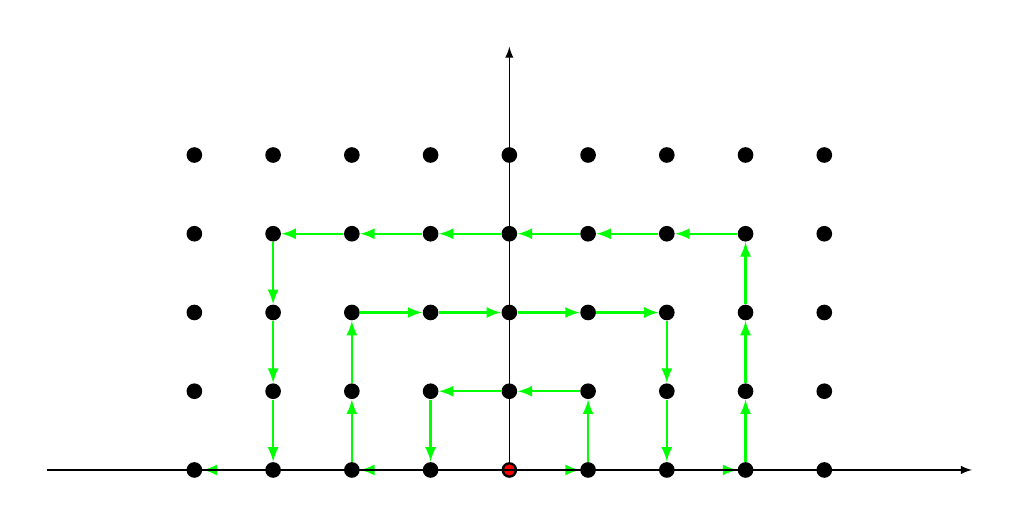
\begin{tikzpicture}
		\foreach \x[count=\x] in {0,1,2,3,4}{
			\node[fill,circle,inner sep=2pt] (x\x) at (-4,\x){};
		}
		
		\foreach \x[count=\x] in {0,1,2,3,4}{
			\node[fill,circle,inner sep=2pt] (a\x) at (-3,\x){};
		}
		
		\foreach \x[count=\x] in {0,1,2,3,4}{
			\node[fill,circle,inner sep=2pt] (b\x) at (-2,\x){};
		}
		
		\foreach \x[count=\x] in {0,1,2,3,4}{
			\node[fill,circle,inner sep=2pt] (c\x) at (-1,\x){};
		}
		
		\foreach \x[count=\x] in {0,1,2,3,4}{
			\node[fill,circle,inner sep=2pt] (d\x) at (0,\x){};
		}
		
		\foreach \x[count=\x] in {0,1,2,3,4}{
			\node[fill,circle,inner sep=2pt] (e\x) at (1,\x){};
		}
		
		\foreach \x[count=\x] in {0,1,2,3,4}{
			\node[fill,circle,inner sep=2pt] (f\x) at (2,\x){};
		}
		
		\foreach \x[count=\x] in {0,1,2,3,4}{
			\node[fill,circle,inner sep=2pt] (g\x) at (3,\x){};
		}
		
		\foreach \x[count=\x] in {0,1,2,3,4}{
			\node[fill,circle,inner sep=2pt] (y\x) at (4,\x){};
		}
		
		\node (d6) at (0,6.5) {};
		\node (z1) at (6,1) {};
		\node (z-1) at (-6,1) {};
		
		\fill[red] (d1) circle (2pt);
		
		\draw[-latex,thick,green] (d1) -- (e1);
		\draw[-latex,thick,green] (e1) -- (e2);
		\draw[-latex,thick,green] (e2) -- (d2);
		\draw[-latex,thick,green] (d2) -- (c2);
		\draw[-latex,thick,green] (c2) -- (c1);
		\draw[-latex,thick,green] (c1) -- (b1);
		\draw[-latex,thick,green] (b1) -- (b2);
		\draw[-latex,thick,green] (b2) -- (b3);
		\draw[-latex,thick,green] (b3) -- (c3);
		\draw[-latex,thick,green] (c3) -- (d3);
		\draw[-latex,thick,green] (d3) -- (e3);
		\draw[-latex,thick,green] (e3) -- (f3);
		\draw[-latex,thick,green] (f3) -- (f2);
		\draw[-latex,thick,green] (f2) -- (f1);
		\draw[-latex,thick,green] (f1) -- (g1);
		\draw[-latex,thick,green] (g1) -- (g2);
		\draw[-latex,thick,green] (g2) -- (g3);
		\draw[-latex,thick,green] (g3) -- (g4);
		\draw[-latex,thick,green] (g4) -- (f4);
		\draw[-latex,thick,green] (f4) -- (e4);
		\draw[-latex,thick,green] (e4) -- (d4);
		\draw[-latex,thick,green] (d4) -- (c4);
		\draw[-latex,thick,green] (c4) -- (b4);
		\draw[-latex,thick,green] (b4) -- (a4);
		\draw[-latex,thick,green] (a4) -- (a3);
		\draw[-latex,thick,green] (a3) -- (a2);
		\draw[-latex,thick,green] (a2) -- (a1);
		\draw[-latex,thick,green] (a1) -- (x1);
		\draw[-latex] (z-1) -- (z1);
		\draw[-latex] (d1) -- (d6);
		\end{tikzpicture}
	\end{center}
\end{frame}

\begin{frame}\frametitle{Countable?}\vspace{-3ex}
	\[|\mathbb{N}|=|\mathbb{Z}\times\mathbb{Z}|\]
	
	\begin{center}
		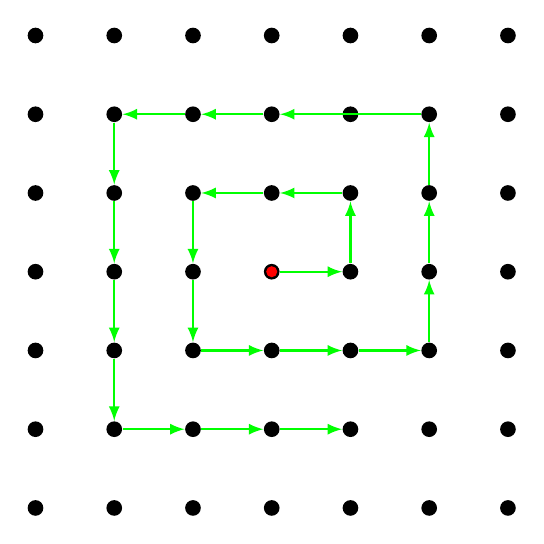
\begin{tikzpicture}
		\foreach \x[count=\x] in {-3,-2,-1,0,1,2,3}{
			\node[fill,circle,inner sep=2pt] (a\x) at (-3,\x){};
		}
		
		\foreach \x[count=\x] in {-3,-2,-1,0,1,2,3}{
			\node[fill,circle,inner sep=2pt] (b\x) at (-2,\x){};
		}
		
		\foreach \x[count=\x] in {-3,-2,-1,0,1,2,3}{
			\node[fill,circle,inner sep=2pt] (c\x) at (-1,\x){};
		}
		
		\foreach \x[count=\x] in {-3,-2,-1,0,1,2,3}{
			\node[fill,circle,inner sep=2pt] (d\x) at (0,\x){};
		}
		
		\foreach \x[count=\x] in {-3,-2,-1,0,1,2,3}{
			\node[fill,circle,inner sep=2pt] (e\x) at (1,\x){};
		}
		
		\foreach \x[count=\x] in {-3,-2,-1,0,1,2,3}{
			\node[fill,circle,inner sep=2pt] (f\x) at (2,\x){};
		}
		
		\foreach \x[count=\x] in {-3,-2,-1,0,1,2,3}{
			\node[fill,circle,inner sep=2pt] (g\x) at (3,\x){};
		}
		
		\fill[red] (d1) circle (2pt);
		
		\draw[-latex,thick,green] (d1) -- (e1);
		\draw[-latex,thick,green] (e1) -- (e2);
		\draw[-latex,thick,green] (e2) -- (d2);
		\draw[-latex,thick,green] (d2) -- (c2);
		\draw[-latex,thick,green] (c2) -- (c1);
		\draw[-latex,thick,green] (c1) -- (c0);
		\draw[-latex,thick,green] (c0) -- (d0);
		\draw[-latex,thick,green] (d0) -- (e0);
		\draw[-latex,thick,green] (e0) -- (f0);
		\draw[-latex,thick,green] (f0) -- (f1);
		\draw[-latex,thick,green] (f1) -- (f2);
		\draw[-latex,thick,green] (f2) -- (f3);
		\draw[-latex,thick,green] (f3) -- (d3);
		\draw[-latex,thick,green] (d3) -- (c3);
		\draw[-latex,thick,green] (c3) -- (b3);
		\draw[-latex,thick,green] (b3) -- (b2);
		\draw[-latex,thick,green] (b2) -- (b1);
		\draw[-latex,thick,green] (b1) -- (b0);
		\draw[-latex,thick,green] (b0) -- (b-1);
		\draw[-latex,thick,green] (b-1) -- (c-1);
		\draw[-latex,thick,green] (c-1) -- (d-1);
		\draw[-latex,thick,green] (d-1) -- (e-1);
		\end{tikzpicture}
	\end{center}
\end{frame}

\begin{frame}\frametitle{$|\mathbb{N}|=|\mathbb{Q}|$}
	\begin{figure}
		\includegraphics[width=.9\textwidth,angle=0,origin=c]{img/nq}
	\end{figure}
	\[|\mathbb{N}|=|\mathbb{Z}|=|2^{<\omega}|=|\mathbb{N}\times\mathbb{N}|=|\mathbb{Z}\times\mathbb{N}|=|\mathbb{Z}\times\mathbb{Z}|=|\mathbb{Q}|\]
\end{frame}

\begin{frame}\frametitle{$|\mathbb{N}|=|\mathbb{Q}^+|$}
	\begin{columns}
		\column{0.5\textwidth}
			\begin{figure}\vspace{-17pt}
				\resizebox{\textwidth}{!}{
					\begin{minipage}{\textwidth}
						\begin{tikzpicture}
						\matrix(m)[green, matrix of math nodes, column sep=0.7cm,row sep=0.7cm, ampersand replacement=\&]{
							\dfrac{1}{1} \& \dfrac{1}{2} \& \dfrac{1}{3} \& \dfrac{1}{4} \& \cdots\\
							\dfrac{2}{1} \& \dfrac{2}{2} \& \dfrac{2}{3} \& \dfrac{2}{4} \& \cdots\\
							\dfrac{3}{1} \& \dfrac{3}{2} \& \dfrac{3}{3} \& \dfrac{3}{4} \& \cdots\\
							\dfrac{4}{1} \& \dfrac{4}{2} \& \dfrac{4}{3} \& \dfrac{4}{4} \& \cdots\\
							\vdots \& \vdots \& \vdots \& \vdots \& \ddots \&\\
						};
						
						\draw[red,thick,->]
						(m-1-1)edge(m-1-2)
						(m-1-2)edge(m-2-1)
						(m-2-1)edge(m-3-1)
						(m-3-1)edge(m-2-2)
						(m-2-2)edge(m-1-3)
						(m-1-3)edge(m-1-4)
						(m-1-4)edge(m-2-3)
						(m-2-3)edge(m-3-2)
						(m-3-2)edge(m-4-1);
						\end{tikzpicture}
				\end{minipage}}
			\end{figure}
		\column{0.5\textwidth}\vspace{-8pt}
			\begin{figure}
				\includegraphics[width=\textwidth,angle=0,origin=c]{img/nqonce}
			\end{figure}\vspace{-8pt}
			\[x\mapsto\frac{1}{\lfloor x\rfloor+1-\{x\}}\]
	\end{columns}
\end{frame}

\begin{frame}\frametitle{\href{https://zhuanlan.zhihu.com/p/27078717}{Hilbert's Hotel}}
	\begin{problem}[Hilbert's Hotel]
		Consider a hypothetical hotel with a countably infinite number of rooms, all of which are occupied.
		\begin{enumerate}
			\item Finitely many new guests.
			\item Infinitely many new guests.
			\item Infinitely many buses with infinitely many guests each.
		\end{enumerate}
	\end{problem}
	\[
		\begin{tabu}{*{10}c}
			\Xcline{1-10}{2pt}
			&\fbox{$\strut{\odot\Delta\odot}$}&\fbox{$\strut{\odot\Delta\odot}$}&\fbox{$\strut{\odot\Delta\odot}$}&\fbox{$\strut{\odot\Delta\odot}$}&\fbox{$\strut{\odot\Delta\odot}$}&\fbox{$\strut{\odot\Delta\odot}$}&\fbox{$\strut{\odot\Delta\odot}$}&\cdots&\\
			\Xcline{1-10}{2pt}
			\vspace*{-10pt}\\
			&\sideset{^\circledcirc}{^\circledcirc}{\operatorname{\hat{o}}}&\sideset{^\circledcirc}{^\circledcirc}{\operatorname{\hat{o}}}&\sideset{^\circledcirc}{^\circledcirc}{\operatorname{\hat{o}}}&\sideset{^\circledcirc}{^\circledcirc}{\operatorname{\hat{o}}}&\sideset{^\circledcirc}{^\circledcirc}{\operatorname{\hat{o}}}&\sideset{^\circledcirc}{^\circledcirc}{\operatorname{\hat{o}}}&\sideset{^\circledcirc}{^\circledcirc}{\operatorname{\hat{o}}}&\cdots&\\
			&\sideset{^\circledcirc}{^\circledcirc}{\operatorname{\hat{o}}}&\sideset{^\circledcirc}{^\circledcirc}{\operatorname{\hat{o}}}&\sideset{^\circledcirc}{^\circledcirc}{\operatorname{\hat{o}}}&\sideset{^\circledcirc}{^\circledcirc}{\operatorname{\hat{o}}}&\sideset{^\circledcirc}{^\circledcirc}{\operatorname{\hat{o}}}&\sideset{^\circledcirc}{^\circledcirc}{\operatorname{\hat{o}}}&\sideset{^\circledcirc}{^\circledcirc}{\operatorname{\hat{o}}}&\cdots&\\
			&\sideset{^\circledcirc}{^\circledcirc}{\operatorname{\hat{o}}}&\sideset{^\circledcirc}{^\circledcirc}{\operatorname{\hat{o}}}&\sideset{^\circledcirc}{^\circledcirc}{\operatorname{\hat{o}}}&\sideset{^\circledcirc}{^\circledcirc}{\operatorname{\hat{o}}}&\sideset{^\circledcirc}{^\circledcirc}{\operatorname{\hat{o}}}&\sideset{^\circledcirc}{^\circledcirc}{\operatorname{\hat{o}}}&\sideset{^\circledcirc}{^\circledcirc}{\operatorname{\hat{o}}}&\cdots&\\
			&\vdots&\vdots&\vdots&\vdots&\vdots&\vdots&\vdots&\ddots&
		\end{tabu}
	\]
\end{frame}

\begin{frame}\frametitle{The set of real numbers is uncountable}
	\begin{center}
		Is every set countable?
	\end{center}
	\begin{theorem}[Cantor]
		\[|\mathbb{R}|>|\mathbb{N}|\]
	\end{theorem}
\setlength\abovedisplayskip{0pt}
\setlength\belowdisplayskip{0pt}
	\begin{proof}
		\[
		\begin{array}{rlllll}
		0\;.&\textcolor{red}{r_{11}}&r_{12}&r_{13}&r_{14}&\dots\\
		0\;.&r_{21}&\textcolor{red}{r_{22}}&r_{23}&r_{24}&\dots\\
		0\;.&r_{31}&r_{32}&\textcolor{red}{r_{33}}&r_{34}&\dots\\
		0\;.&r_{41}&r_{42}&r_{43}&\textcolor{red}{r_{44}}&\dots\\
		\vdots\; & \;\vdots&\;\vdots&\;\vdots\;&\vdots&\textcolor{red}{\ddots}
		\end{array}
		\]
		Let $d=0.d_1 d_2\dots$ where
		\[d_n=9-r_{nn}\]
	\end{proof}
\end{frame}

\begin{frame}\frametitle{Continuum}
	\begin{columns}
		\column{.6\textwidth}
		\onslide<1-2>
			\centering\resizebox{.9\textwidth}{!}{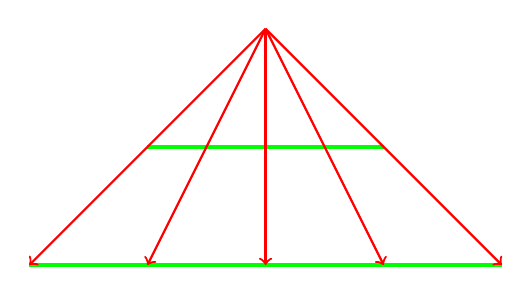
\begin{tikzpicture}
				%\draw [help lines] (0,0) grid (10,5);
				\draw[-,very thick,green] (-3,0) -- (3,0);
				\draw[-,very thick,green] (-1.5,1.5) -- (1.5,1.5);
				\draw[->,thick,red] (0,3) -- (-3,0);
				\draw[->,thick,red] (0,3) -- (3,0);
				\draw[->,thick,red] (0,3) -- (0,0);
				\draw[->,thick,red] (0,3) -- (-1.5,0);
				\draw[->,thick,red] (0,3) -- (1.5,0);
				\end{tikzpicture}}
		\onslide<2->
			\centering\resizebox{\textwidth}{!}{
				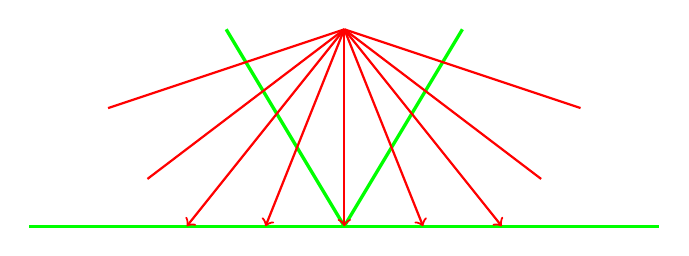
\begin{tikzpicture}
				%\draw [help lines] (0,0) grid (10,5);
				%\draw[ultra thick] (-2.5,2.5) arc (-180:0:2.5)-- (2.5,2.5) ;
				\draw[-,very thick,green] (-4,0) -- (4,0);
				\draw[-,very thick,green] (-1.5,2.5) -- (0,0);
				\draw[-,very thick,green] (1.5,2.5) -- (0,0);
				\draw[->,thick,red] (0,2.5) -- (-2,0);
				\draw[->,thick,red] (0,2.5) -- (2,0);
				\draw[->,thick,red] (0,2.5) -- (0,0);
				\draw[->,thick,red] (0,2.5) -- (-1,0);
				\draw[->,thick,red] (0,2.5) -- (1,0);
				\draw[-,thick,red] (0,2.5) -- (-2.5,0.6);
				\draw[-,thick,red] (0,2.5) -- (2.5,0.6);
				\draw[-,thick,red] (0,2.5) -- (-3,1.5);
				\draw[-,thick,red] (0,2.5) -- (3,1.5);
				\end{tikzpicture}
			}
		\column{.45\textwidth}
		\onslide<3->
			\centering\resizebox{\textwidth}{!}{
				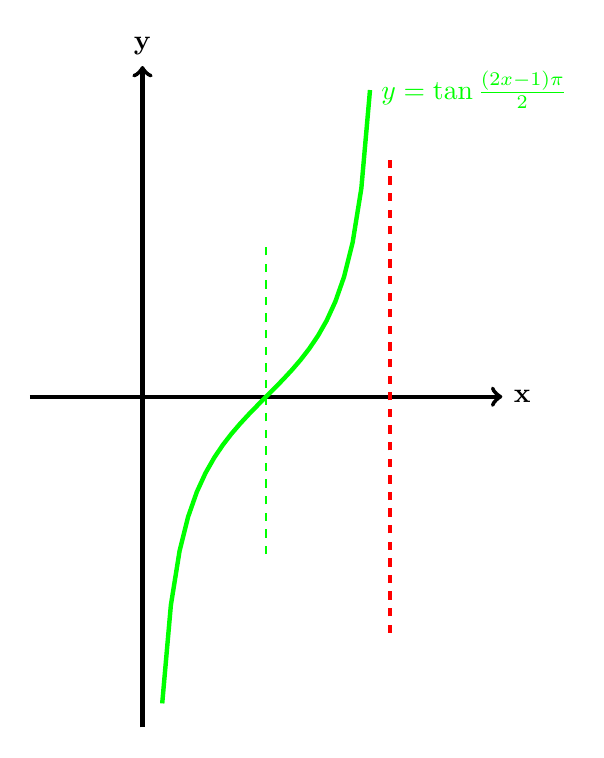
\begin{tikzpicture}[domain=-4:7] [scale=0.8]
				\draw[ultra thick, ->] (-3,0) -- (3,0) node[right] {$\mathbf{x}$};
				\draw[dashed,thick,green] (0,-2) -- (0,2);
				\draw[dashed, ultra thick,red] (1.57,-3) -- (1.57,3);
				\draw[ultra thick,->] (-1.57,-4.2) -- (-1.57,4.2) node[above] {$\mathbf{y}$};
				\draw[ultra thick,color=green] plot[domain=-.42*pi:.42*pi] (\x,{tan(\x r)}) node[right] {$y=\tan\frac{(2x-1)\pi}{2}$};
				\end{tikzpicture}
			}
	\end{columns}
\end{frame}

\begin{frame}\frametitle{Continuum}
\begin{columns}
\column{.42\textwidth}
\[f: (0,1]\biject(0,1)\]
\[
f(x)\coloneqq 
\begin{cases}
\frac{3}{2}-x&\mbox{for } \frac{1}{2}<x\leq 1\\
\frac{3}{4}-x&\mbox{for } \frac{1}{4}<x\leq \frac{1}{2}\\
\frac{3}{8}-x&\mbox{for } \frac{1}{8}<x\leq \frac{1}{4}\\
\quad\vdots
\end{cases}
\]
\[
f(x)\coloneqq 
\begin{cases}
\frac{x}{x+1}&\mbox{if } \exists n\in\mathbb{N}: x=\frac{1}{n}\\
x&\mbox{otherwise }
\end{cases}
\]
\column{.47\textwidth}
\begin{figure}
	\includegraphics[width=\textwidth,angle=0,origin=c]{img/biject01.pdf}
\end{figure}
\end{columns}
\end{frame}

\begin{frame}\frametitle{Continuum}
	\centering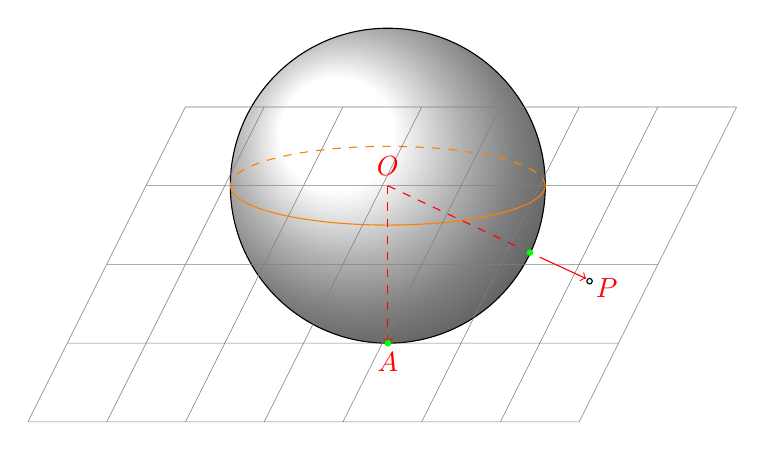
\begin{tikzpicture}[point/.style={draw, circle, fill=green!10, inner sep=0.7pt}]
	\def\rad{2cm}
	\coordinate (O) at (0,0); 
	\coordinate (N) at (0,-\rad); 
	
	\filldraw[ball color=white!30] (O) circle [radius=\rad];
	\draw[dashed,orange] 
	(\rad,0) arc [start angle=0,end angle=180,x radius=\rad,y radius=5mm];
	\draw[orange]
	(\rad,0) arc [start angle=0,end angle=-180,x radius=\rad,y radius=5mm];
	\begin{scope}[xslant=0.5,yshift=\rad,xshift=-2]
	\draw [help lines] (-3,-5) grid (4,-1);
	\node [red] (P) at (3.5,-3.3) {$P$};
	\node [red] (Q) at (2.3,-2.85) {};
	\end{scope}
	\draw[red,dashed,->] (O) node[above] {$O$} -- (N) node[below] {$A$};
	\node[point,green] at (N) {};
	\draw[red,dashed] (O) -- (Q);
	\draw[red,->] (Q) -- (P);
	\node[point,above=2.5pt, left=5pt] at (P) {};
	\node[point,green] at (Q) {};
	\end{tikzpicture}
\end{frame}

\begin{frame}\frametitle{Continuum}
	\begin{theorem}
		\[|\mathbb{R}|=|\mathbb{R}\times\mathbb{R}|\]
	\end{theorem}
	\begin{proof}
	\[
		\begin{tabu}{llrrrr}
		x=&0.3&01&2&007&08\dots\\
		y=&0.009&2&05&1&0003\dots
		\end{tabu}
	\]
		\[z=0.3\;009\;01\;2\;2\;05\;007\;1\;08\;0003\;\dots\]
	\end{proof}
\end{frame}

\begin{frame}\frametitle{Continuum}\centering
	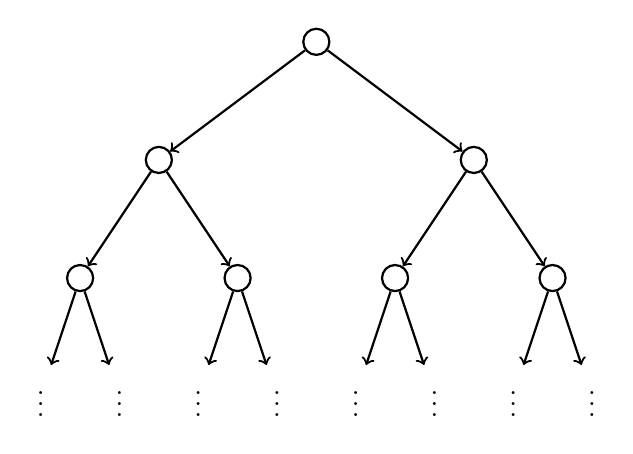
\begin{tikzpicture}[->, auto, thick, level 1/.style={sibling distance=40mm},
	level 2/.style={sibling distance=20mm},
	level 3/.style={sibling distance=10mm}
	]
	
	\node [circle,draw] (z){}
	child {node [circle,draw] (a) {}
		child {node [circle,draw] (b) {}
			child {node {$\vdots$}
			} 
			child {node {$\vdots$}}
		}
		child {node [circle,draw] (g) {}
			child {node {$\vdots$}}
			child {node {$\vdots$}}
		}
	}
	child {node [circle,draw] (j) {}
		child {node [circle,draw] (k) {}
			child {node {$\vdots$}}
			child {node {$\vdots$}}
		}
		child {node [circle,draw] (l) {}
			child {node {$\vdots$}}
			child {node (c){$\vdots$}
			}
		}
	};
	\end{tikzpicture}
	\[[0,1]=\left\{\sum\limits_{n=1}^\infty\dfrac{x_n}{2^n}: x_n=0\vee x_n=1\right\}\]
\end{frame}

\begin{frame}\frametitle{Cantor's Continuum Hypothesis}
\begin{block}{Cantor's Continuum Hypothesis (CH)}
\[2^{\aleph_0}\;\textcolor{red}{\stackrel{?}{=}}\;\aleph_1\]
\end{block}
\begin{figure}[H]
\includegraphics[width=.8\textwidth]{img/cantor-ch}
\end{figure}
\end{frame}


%%%%%%%%%%%%%%%%%%%%%%%%%%%%%%%
\section{Propositional Logic}
%%%%%%%%%%%%%%%%%%%%%%%%%%%%%%%


\begin{frame}\frametitle{Logic $\to$ Truth}
	\begin{quote}
		\emph{Truth} points the way for logic, just as beauty does for aesthetics, and goodness for ethics.\par
		\hfill --- \textsl{Frege}
	\end{quote}
	\centerline{\xymatrix@C=1pc{
					*+++[o][F=]{\textbf{\underline{\textcolor{yellow}{\text{Form}}}}}&&&&&&*+++[o][F=]{\textbf{\underline{\textcolor{yellow}{\text{Form}}}}}\\
					&&&&
					\ar@1{<--}^*++[F-]{\text{\footnotesize endow}} "1,7";"5,4"
					&&&\\
					\ar@1{-->}_*++[F-]{\text{\footnotesize suspend}} "1,1";"5,4"
					&&&&&\\
					\ar@1{->}^*++[F-]{\textcolor{red}{\text{\footnotesize transform}}} "1,1";"1,7"\\
					&&&*+++[F-]{\textbf{\textcolor{yellow}{Meaning}}}&&}}
\end{frame}

\begin{frame}\frametitle{}
\begin{gather*}
\textcolor{red}{{\text{Natural Language}}}\\
\MapDown{\text{represents}}\\
\fbox{Formal Language (Syntax)}\\
\bigg{\Downarrow}\rlap{\text{\footnotesize expresses}}\\
\fbox{Theory (calculus $\vdash$)}\\
\bigg{\Downarrow}\llap{\text{\footnotesize interprets\;\;\;}}\bigg{\Uparrow}\rlap{\text{\footnotesize characterizes}}\\
\fbox{Models (semantics $\vDash$)}\\
\MapUp{\text{represents}}\\
\qquad\qquad\dots\dots\dots\dots\dots\dots\dots\dots\dots\dots\dots\dots\dots\dots \text{semantic gap}\\
\textcolor{red}{{\text{Real World}}}
\end{gather*}
\end{frame}

%%%%%%%%%%%%%%%%%%%%%%%%%%%%%%%
\subsection{Syntax}
%%%%%%%%%%%%%%%%%%%%%%%%%%%%%%%

\begin{frame}\frametitle{Propositional Logic}
	\begin{itemize}
		\item Language.
		
		Building blocks of propositional logic language.
		\item Syntax.
		
		Propositional symbols and propositional formulae.
		\item Semantics.
		
		Assign ``meaning'' to propositional formulae by first assigning ``meaning'' to propositional symbols.
		\item Calculus.
		
		Axioms and inference rules.
	\end{itemize}
\end{frame}

\begin{frame}\frametitle{Syntax}
		\begin{block}{Language}
			\[\mathscr{L}^0\coloneqq \{\textcolor{green}{\neg},\wedge,\vee,\textcolor{green}{\to},\leftrightarrow,(,)\}\cup\mathcal{P}\]
		\end{block}
		where $\mathcal{P}\coloneqq \{p_1,\dots,p_n,(\dots)\}$.
		\begin{block}{Well-Formed Formula $\mathrm{wff}$}
			\[A\Coloneqq p\mid \textcolor{green}{(\neg A)}\mid (A\wedge A)\mid (A\vee A)\mid \textcolor{green}{(A\to A)}\mid (A\leftrightarrow A)\]
		\end{block}
		\begin{itemize}
			\item $\bot\coloneqq (A\wedge(\neg A))$
			\item $\top\coloneqq (\neg\bot)$
		\end{itemize}
		\begin{block}{Example}
			\begin{itemize}
				\item Lily is (not) beautiful.
				\item If wishes are horses, then beggars will ride.
				\item Lily is beautiful and/or/iff $2$ is not a prime number.
			\end{itemize}
		\end{block}
\end{frame}

\begin{frame}\frametitle{Well-Formed Formula}
\setlength\abovedisplayskip{0pt}
\setlength\belowdisplayskip{0pt}\vspace{-2pt}\centering
	\begin{overpic}[scale=0.45]{img/panda.png}
	\put(1,75){\textcolor{yellow}{\footnotesize\textbf{\textcolor{green!30!black}{A panda eats\textcolor{red}{\Large,}shoots and leaves.}}}}
	\end{overpic}\vspace{-3ex}
	\begin{definition}[Formula-Building Operator]
		\begin{columns}
			\column{0.3\textwidth}
				\begin{align*}
				\mathcal{E}_\neg(A)&\coloneqq (\neg A)\\
				\mathcal{E}_\wedge(A, B)&\coloneqq (A\wedge B)\\
				\mathcal{E}_\vee(A, B)&\coloneqq (A\vee B)\\
				\mathcal{E}_\to(A, B)&\coloneqq (A\to B)\\
				\mathcal{E}_\leftrightarrow(A, B)&\coloneqq (A\leftrightarrow B)
				\end{align*}
			\column{0.3\textwidth}
				\boxed{\vbox{
					\begin{align*}
					\mathcal{E}_\neg(A)&\coloneqq \neg A\\
					\mathcal{E}_\wedge(A, B)&\coloneqq \wedge A B\\
					\mathcal{E}_\vee(A, B)&\coloneqq \vee A B\\
					\mathcal{E}_\to(A, B)&\coloneqq \to A B\\
					\mathcal{E}_\leftrightarrow(A, B)&\coloneqq \leftrightarrow A B
					\end{align*}}}
		\end{columns}
	\end{definition}
\end{frame}

\begin{frame}\frametitle{Well-Formed Formula}
\setlength\abovedisplayskip{0pt}
\setlength\belowdisplayskip{0pt}
	\begin{definition}[Construction Sequence]
		A construction sequence $(C_1,\dots, C_n)$ is a finite sequence of expressions s.t. for each $i\leq n$ we have at least one of 
		\begin{align*}
		&C_i=p_i\quad\text{for some $i$}\\
		&C_i=(\neg C_j)\quad\text{for some $j$}\\
		&C_i=(C_j\star C_k)\quad\text{for some $j<i, k<i$}, \mbox{ where }\star\in\{\wedge,\vee,\to,\leftrightarrow\}.
		\end{align*}
	\end{definition}
	\begin{definition}[Well-Formed Formula]
	A formula $A$ is a well-formed formula (wff) iff there is some construction sequence $(C_1,\dots, C_n)$ and $C_n=A$.
	\end{definition}\vspace*{-3ex}
\begin{align*}
\mathrm{wff}_0&\coloneqq \{p_1,p_2,\dots\}\\
\mathrm{wff}_{n+1}&\coloneqq \mathrm{wff}_n\cup\big\{(\neg A): A\in\mathrm{wff}_n\big\}\cup\big\{(A\to B): A, B\in\mathrm{wff}_n\big\}\\
\mathrm{wff}_*&\coloneqq \bigcup\limits_{n\in\mathbb{N}}\mathrm{wff}_n
\end{align*}
\end{frame}

\begin{frame}\frametitle{Generation --- Bottom Up vs Top Down}
\setlength\abovedisplayskip{0pt}
\setlength\belowdisplayskip{0pt}
	\begin{block}{Problem}
		Given a class $\mathcal{F}$ of functions over $U$, how to \textcolor{yellow}{generate} a certain subset of $U$ by starting with some initial elements $B\subset U$?
	\end{block}
			\begin{block}{Bottom Up}\vspace{-4pt}
				\begin{align*}
				C_0&\coloneqq B\\ C_{n+1}&\coloneqq C_n\cup\bigcup\limits_{f\in\mathcal{F}}\left\{f(\mathbf{x}): \mathbf{x}\in C_n\right\}\qquad\operatorname{deg}(\mathbf{x})\coloneqq \mu n\left[\mathbf{x}\in C_n\right]\\
				C_*&\coloneqq \bigcup\limits_{n\in\mathbb{N}} C_n
				\end{align*}
			\end{block}
			\begin{block}{Top Down}
				\begin{itemize}
					\item A set $S$ is \textcolor{green}{closed under a function} $f$ if for all $\mathbf{x}$: $\mathbf{x}\in S\to f(\mathbf{x})\in S$.
					\item A set $S$ is \textcolor{yellow}{inductive} if $B\subset S$ and for all $f\in\mathcal{F}$: $S$ is closed under $f$.
					\item $C^*\coloneqq \bigcap\{S: S\mbox{ is inductive}\}$
				\end{itemize}
			\end{block}
\end{frame}

\begin{frame}\frametitle{Bottom Up vs Top Down}
	\begin{block}{How many bottles of beer can you buy with $\$10$?}
		\begin{itemize}
		\item $\$2$ can buy $1$ bottle of beer.
		\item $4$ bottle caps can be exchanged for $1$ bottle of beer.
		\item $2$ empty bottles can be exchanged for $1$ bottle of beer.
		\end{itemize}
	\end{block}
\end{frame}

\begin{frame}\frametitle{Generation --- Bottom Up vs Top Down}
\setlength\abovedisplayskip{0pt}
\setlength\belowdisplayskip{0pt}
\begin{block}{Example}
		Let $B\coloneqq \{0\}, \mathcal{F}\coloneqq \{S,P\}, S(x)\coloneqq x+1, P(x)\coloneqq x-1$
		\[C_*=\{\dots,-2,-1,0,1,2,\dots\}\]
		There is more than one way of obtaining a member of $C_*$, e.g. $1=S(0)=S(P(S(0)))$.
\end{block}
\begin{theorem}[Bottom up and Top down]
	\[C_*=C^*\]
\end{theorem}
\begin{proof}
	($C^*\subset C_*$): to show $C_*$ is inductive.\\
	($C_*\subset C^*$): consider $x\in C_*$ and a construction sequence $(x_1,\dots,x_n)$ for $x$. First $x_1\in B\subset C^*$. If for all $j<i$ we have $x_j\in C^*$, then $x_i\in C^*$. By induction, $x_1,\dots,x_n\in C^*$.
\end{proof}
\end{frame}

\begin{frame}\frametitle{Induction Principle for wff}
	\begin{theorem}[Induction Principle]
		Let $P$ be a property of formulae, satisfying
		\begin{itemize}
		\item every atomic formula has property $P$, and
		\item property $P$ is closed under all the formula-building operations,
		\end{itemize}
		then every formula has property $P$.
	\end{theorem}
	\begin{proof}
		\[\mathrm{wff}_*=\mathrm{wff}^*\subset P\]
	\end{proof}
	\[P(0)\wedge\forall k\in\mathbb{N}(P(k)\to P(k+1))\to\forall n\in\mathbb{N} P(n)\]
	\[P(k)\coloneqq P(\mathrm{wff}_k)\]
\end{frame}

\begin{frame}\frametitle{Induction vs Recursion}
\begin{figure}[H]
\includegraphics[width=.5\textwidth]{img/hanoi.pdf}
\end{figure}
\begin{center}
$P(n)\coloneqq $ ``$n$ rings needs $2^n-1$ moves.''
\end{center}
\begin{block}{}
\begin{enumerate}
\item If ever you leave milk one day, be sure and leave it the next day as well.
\item Leave milk today.
\end{enumerate}
\end{block}
\centering
\fbox{Leave milk today and read this note again tomorrow.}
\end{frame}

\begin{frame}\frametitle{Subformula}
	\begin{definition}[Subformula]
		The set $\operatorname{Sub}(A)$ of subformulae of a wff $A$ is the smallest set $\Gamma$ that satisfies
		\begin{enumerate}
			\item $A\in\Gamma$
			\item $\neg B\in\Gamma\implies B\in\Gamma$
			\item $B\to C\in\Gamma\implies B, C\in\Gamma$
		\end{enumerate}
	\end{definition}
	\begin{block}{}
		\[
		\operatorname{Sub}(A)\coloneqq 
		\begin{cases}
		 A &\text{if}\; A=p\\
		\{A\}\cup \operatorname{Sub}(B) &\text{if}\; A=\neg B\\
		\{A\}\cup \operatorname{Sub}(B)\cup \operatorname{Sub}(C) &\text{if}\; A=B\to C
		\end{cases}
		\]
	\end{block}
\end{frame}

\begin{frame}\frametitle{Unique Readability, Unique Tree}\vspace{-21pt}
	\begin{figure}
		\[((\neg p)\wedge q)\to(p\wedge(q\vee(\neg r)))\]
		\begin{tikzpicture}[level distance=12mm,outer sep=1mm,inner sep=0,
		level 1/.style={sibling distance=20mm},
		level 2/.style={sibling distance=15mm},
		level 3/.style={sibling distance=15mm},
		level 4/.style={sibling distance=15mm}]
		\begin{scope}[nodes={green,minimum size=5mm}]
		\node (e) {$\to$}
		child { node (l) {$\wedge$}
			child { node (ll) {$\neg$}
				child { node (lll) {$\textcolor{red}{p}$}
				}
			}
			child { node (lr) {\!\!\!\!$\textcolor{red}{q}$}
			}
		}
		child { node (r) {$\wedge$}
			child { node (rl) {\;\;\;$\textcolor{red}{p}$}
			}
			child { node (rr) {$\vee$}
				child { node (rrl) {$\textcolor{red}{q}$}
				}
				child { node (rrr) {$\neg$}
					child { node (rrrr) {$\textcolor{red}{r}$}
					}
				}
			}
		};
		\end{scope}
		\end{tikzpicture}
	\end{figure}
	\centering subformula vs subtree
\end{frame}

\begin{frame}\frametitle{Omitting Parentheses}
	\begin{enumerate}
		\item The outermost parentheses need not be explicitly mentioned.
		\item We order the boolean connectives according to decreasing binding strength: $\neg, \wedge, \vee, \to, \leftrightarrow$.
		\item Where one connective symbol is used repeatedly, grouping is to the right.
	\end{enumerate}
	\[1+2*3\]
\end{frame}

%%%%%%%%%%%%%%%%%%%%%%%%%%%%%%%
\subsection{Semantics}
%%%%%%%%%%%%%%%%%%%%%%%%%%%%%%%

\begin{frame}\frametitle{Assignment}
	\begin{itemize}
		\item A truth assignment for $\mathscr{L}^0$ is a function
		\[\nu:\mathcal{P}\to\{0,1\}\]
		\item Such a truth assignment can be uniquely extended to $\overline{\nu}:\mathrm{wff}\to\{0,1\}$ satisfying the following condition:\\
		\begin{enumerate}
			\item $\overline{\nu}(p)=\nu(p)$ for $p\in\mathcal{P}$
			\item $\overline{\nu}(\neg A)=1-\overline{\nu}(A)$
			\item $\overline{\nu}(A\wedge B)=\min\{\overline{\nu}(A),\overline{\nu}(B)\}$
			\item $\overline{\nu}(A\vee B)=\max\{\overline{\nu}(A),\overline{\nu}(B)\}$
			\item $\overline{\nu}(A\to B)=1-\overline{\nu}(A)+\overline{\nu}(A)\cdot\overline{\nu}(B)$
			\item $\overline{\nu}(A\leftrightarrow B)=\overline{\nu}(A)\cdot\overline{\nu}(B)+(1-\overline{\nu}(A))\cdot(1-\overline{\nu}(B))$
		\end{enumerate}
	\end{itemize}
\end{frame}

\begin{frame}\frametitle{Truth Table \& Truth/Boolean Function}
			\[
			\begin{tabu}{c|c}
			\hline
			\textcolor{yellow}{p} & \textcolor{green}{\neg p}\\
			\hline
			0 & 1\\
			1 & 0\\
			\hline
			\end{tabu}\qquad
			\begin{tabu}{cc|c|c|c|c}
				\hline
				\textcolor{yellow}{p} & \textcolor{yellow}{q} & p\wedge q & p\vee q & \textcolor{green}{p\to q} & p\leftrightarrow q\\
				\hline
				0 & 0 & 0 & 0 & 1 & 1\\
				0 & 1 & 0 & 1 & 1 & 0\\
				1 & 0 & 0 & 1 & 0 & 0\\
				1 & 1 & 1 & 1 & 1 & 1\\
				\hline
			\end{tabu}
			\]
		\begin{block}{Example}
			\begin{itemize}
				\item If $0=1$, then Russell is God.\\
				\item Snow is white iff $1+1=2$.
			\end{itemize}
		\end{block}
\end{frame}

\begin{frame}\frametitle{Material Implication vs Cognition}
	\begin{block}{}
		Which cards must be turned over to test the idea that if a card shows an even number on one face, then its opposite face is red?
	\end{block}
	\includegraphics[width=\textwidth]{img/wason.png}
	\begin{block}{}
		No drinking under 18!
	\end{block}
\end{frame}

\begin{frame}\frametitle{Tautology}
		If lily is beautiful, then the fact that $2$ is a prime number implies lily is beautiful.
		\[
			\begin{tabu}{cc|c|c}
				\hline
				p & q & q\to p & p\to q\to p\\
				\hline
				0 & 0 & 1 & 1\\
				0 & 1 & 0 & 1\\
				1 & 0 & 1 & 1\\
				1 & 1 & 1 & 1\\
				\hline
			\end{tabu}
		\]
		\begin{center}
			$2^n$ truth assignments for a set of
			$n$ propositional symbols.
		\end{center}
		\begin{itemize}
			\item $\nu\vDash A$ if $\overline{\nu}(A)=1$.
			\item \textcolor{green}{Logical Consequence.} \textcolor{yellow}{$\Gamma\vDash A$} if for any truth assignment $\nu$ s.t. $(\text{for all}\; B\in\Gamma: \nu\vDash B)\implies\nu\vDash A$.
			\item \textcolor{green}{Tautology.} \textcolor{yellow}{$\vDash A$ if $\emptyset\vDash A$}.
		\end{itemize}
\end{frame}

\begin{frame}\frametitle{}
\[\vDash (p\to q\to r)\to (p\to q)\to p\to r\]
	\[\tiny
		\begin{tabu}{ccc|c|c|c|c|c|c}
			\hline
			p & q & r & q\to r & p\to q\to r & p\to q & p\to r & (p\to q)\to p\to r & (p\to q\to r)\to (p\to q)\to p\to r\\
			\hline
			0 & 0 & 0 & &&&&& 1\\
			0 & 0 & 1 & &&&&& 1\\
			0 & 1 & 0 & &&&&& 1\\
			0 & 1 & 1 & &&&&& 1\\
			1 & 0 & 0 & &&&&& 1\\
			1 & 0 & 1 & &&&&& 1\\
			1 & 1 & 0 & &&&&& 1\\
			1 & 1 & 1 & &&&&& 1\\
			\hline
		\end{tabu}
	\]
\end{frame}

\begin{frame}\frametitle{Truth Table --- Simplification for Tautology}
	\begin{table}\huge
		\tabcolsep=2pt
		\begin{tabu}{*{24}c}
			&$($&$p$&$\to$&&$q$&$\to$ &$r$&$)$&&$\to$ &&$($&$p$&$\to$ &$q$&$)$&$\to$&&$p$&$\to$ &$r$&&\\
			&&&&&&&&&&$\underline{\mathbf{0}}$&&&&&&&&&&&&&\\
			&&&1&&&&&&&$\mathbf{0}$&&&&&&&$\underline{\mathbf{0}}$&&&&&&\\
			&&&1&&&&&&&$\mathbf{0}$&&&&1&&&$\mathbf{0}$&&&$\underline{\mathbf{0}}$&&&\\
			&&\textcolor{red}{1}&1&&&&\textcolor{red}{0}&&&$\mathbf{0}$&&&\textcolor{red}{1}&$\underline{\mathbf{1}}$&&&$\mathbf{0}$&&\textcolor{red}{1}&$\mathbf{0}$&\textcolor{red}{0}&&\\
			&&\textcolor{red}{1}&$\underline{\mathbf{1}}$&&\textcolor{red}{1}&&\textcolor{red}{0}&&&$\mathbf{0}$&&&\textcolor{red}{1}&$\mathbf{1}$&\textcolor{red}{1}&&$\mathbf{0}$&&\textcolor{red}{1}&$\mathbf{0}$&\textcolor{red}{0}&&\\
			&&\textcolor{red}{1}&$\mathbf{1}$&&\textcolor{red}{1}&$\underline{\mathbf{1}}$&\textcolor{red}{0}&&&$\mathbf{0}$&&&\textcolor{red}{1}&$\mathbf{1}$&\textcolor{red}{1}&&$\mathbf{0}$&&\textcolor{red}{1}&$\mathbf{0}$&\textcolor{red}{0}&&\\
			&&&&&&$\textcolor{red}{\times}$&&&&&&&&&&&&&&&&&
		\end{tabu}
	\end{table}
\end{frame}

\begin{frame}\frametitle{Exercises --- Translation}
		\begin{enumerate}
			\item The answer is $3$ or $6$.
			\item I am not good at logic.
			\item If you can't say it clearly, you don't understand it yourself.
			\item You understand something only if you can formalize it.
			\item I will go out unless it rains.
			\item You can pay by credit card or cheque.
			\item Neither Sarah nor Peter was to blame for the mistake.
			\item I want to buy either a new desktop computer or a laptop, but I have neither the cash nor the credit I need.
			\item If I get in the lift then it breaks, \textcolor{yellow}{and/or} if you get in then the lift breaks. (\textcolor{yellow}{?})\hfill \textcolor{yellow}{(Natural language is ambiguous!)}
			\item If we both get in the lift, then the lift breaks.
			\item $p\vee q\to r\semeq(p\to r)\wedge(q\to r)$
			\item $p\wedge q\to r\semeq(p\to r)\vee(q\to r)$
		\end{enumerate}
\end{frame}

\begin{frame}\frametitle{Example}
	\begin{block}{$\sideset{^\circledcirc}{^\circledcirc}{\operatorname{\hat{o}}}$}
		\begin{enumerate}
			\item The programmer's wife tells him: ``Run to the store and pick up a loaf of bread. If they have eggs, get a dozen.''
			\item The programmer comes home with $12$ loaves of bread.
			\item ``Why did you buy $12$ loaves of bread!?'', his wife screamed.
			\item ``Because they had eggs!''
		\end{enumerate}	
	\end{block}
	\begin{itemize}
		\item wife.
		\[q\wedge(p\to r)\]
		\item programmer.
		\[(\neg p\to q)\wedge(p\to s)\]
	\end{itemize}
\end{frame}

\begin{frame}\frametitle{Exercises --- Validity}
		\begin{columns}
			\column{0.5\textwidth}
				\begin{enumerate}
					\item \textcolor{green}{$p\vee q\semeq\neg p\to q\semeq(p\to q)\to q$}
					\item \textcolor{green}{$p\wedge q\semeq\neg(p\to\neg q)$}
					\item \textcolor{green}{$p\leftrightarrow q\semeq(p\to q)\wedge(q\to p)$}
					\item $p\wedge q\semeq\neg(\neg p\vee\neg q)$
					\item $p\to q\to r\semeq(p\wedge q)\to r$
					\item $p\to q\semeq\neg q\to\neg p$
					\item $p\wedge(q\vee r)\semeq(p\wedge q)\vee(p\wedge r)$
					\item $p\vee(q\wedge r)\semeq(p\vee q)\wedge(p\vee r)$
					\item $\neg(p\vee q)\semeq\neg p\wedge\neg q$
					\item $\neg(p\wedge q)\semeq\neg p\vee\neg q$
					\item $p\semeq p\vee(p\wedge q)$
					\item $p\semeq p\wedge(p\vee q)$
				\end{enumerate}
			\column{0.5\textwidth}
				\begin{enumerate}
					\item \textcolor{red}{$\neg\neg p\to p$}
					\item $p\to\neg\neg p$
					\item \textcolor{red}{$p\vee\neg p$}
					\item $\neg(p\wedge\neg p)$
					\item $p\wedge\neg p\to q$
					\item \textcolor{red}{$(p\to q)\wedge(\neg p\to q)\to q$}
					\item $(p\to q)\wedge(p\to\neg q)\to\neg p$
					\item \textcolor{red}{$(\neg p\to q)\wedge(\neg p\to\neg q)\to p$}
					\item \textcolor{red}{$((p\to q)\to p)\to p$}
				\end{enumerate}
				\begin{enumerate}
					\item $\Gamma, A\vDash B\iff\Gamma\vDash A\to B$
					\item $A\semeq B\iff\vDash A\leftrightarrow B$
					\item $A\vee B, \neg A\vee C\vDash B\vee C$
				\end{enumerate}
		\end{columns}
\end{frame}

\begin{frame}\frametitle{}
	\begin{columns}
		\column{0.3\textwidth}
			\begin{prooftree}
				\AxiomC{$p\to q$}
				\noLine
				\UnaryInfC{$\phantom{p\to} q$}
				\alwaysSingleLine
				\UnaryInfC{$p$}
			\end{prooftree}
		\column{0.3\textwidth}
			\begin{prooftree}
				\AxiomC{$p\to q$}
				\noLine
				\UnaryInfC{$\neg p\phantom{\to q}$}
				\alwaysSingleLine
				\UnaryInfC{$\neg q$}
			\end{prooftree}
		\column{0.3\textwidth}
			\begin{prooftree}
				\AxiomC{$p\vee q$}
				\noLine
				\UnaryInfC{$p$}
				\alwaysSingleLine
				\UnaryInfC{$\neg q$}
			\end{prooftree}
	\end{columns}
	\begin{prooftree}
		\AxiomC{I think, therefore I am}
		\noLine
		\UnaryInfC{I do not think\phantom{foreI am}}
		\alwaysSingleLine
		\UnaryInfC{Therefore I am not}
	\end{prooftree}
	\centerline{\infer{\text{Jerry is innocent}}{\begin{array}{cc}
	\text{Mickey is murdered by Tom or Jerry}\\
	\text{Tom is the killer}
	\end{array}}}
\begin{block}{}
\begin{quote}
	\textcolor{yellow}{By all means marry; if you get a good wife, you'll be happy. If you get a bad one, you'll become a philosopher.} \par\hfill --- \textsl{Socrates}
\end{quote}
\end{block}
\end{frame}

\begin{frame}\frametitle{Example}
\begin{block}{}
好货不贱,贱货不好。
\end{block}
\begin{block}{}
如果把整个太平洋的水倒出,也浇不灭我对你爱情的火焰。
整个太平洋的水倒得出吗?不行。
所以,我不爱你。
\end{block}
\begin{block}{}
如果把整个浴缸的水倒出,也浇不灭我对你爱情的火焰。
整个浴缸的水倒得出吗?可以。
所以,是的,我爱你。
\end{block}
\end{frame}

\begin{frame}\frametitle{Example}
	\begin{block}{}
	\begin{itemize}
		\item 如果你工作,就能挣钱;如果你赋闲在家,就能悠然自在。你要么工作要么赋闲,总之,你能挣钱或者能悠然自在。
		\item 如果你工作,就不能悠然自在;如果你赋闲在家,就不能挣钱。你要么工作要么赋闲,总之,你不能悠然自在或者不能挣钱。
	\end{itemize}
	\end{block}
	\[p\to r, q\to s\vDash p\vee q\to r\vee s\]
	\[p\to\neg s, q\to\neg r\vDash p\vee q\to\neg s\vee\neg r\]
\begin{itemize}
	\item 老婆婆有俩儿子,老大卖阳伞,老二卖雨伞,晴天雨伞不好卖,雨天阳伞不好卖……
	\item 被困失火的高楼,走楼梯会被烧死,跳窗会摔死……
\end{itemize}
\end{frame}

\begin{frame}\frametitle{Example}
	\begin{block}{诉讼悖论}\small
		\begin{itemize}
			\item 曾有师生签订合同:上学期间不收费,学生毕业打赢第一场官司后交学费。
			\item 可学生毕业后并未从事律师职业,于是老师威胁起诉学生。
			\item 老师说:如果我赢了,根据法庭判决,你必须交学费;如果你赢了,根据合同,你也必须交学费。要么我赢要么你赢,你都必须交学费。
			\item 学生说:如果我赢了,根据法庭判决,我不用交学费;如果你赢了,根据合同,我不用交学费。要么我赢要么你赢,我都不用交学费。
		\end{itemize}
	\end{block}
\begin{columns}
\column{.64\textwidth}
	\[w\to p, \neg w\to p, w\vee\neg w\vDash p\]
	\[w\wedge j\to p, \neg w\wedge c\to p, w\vee\neg w\stackrel{?}{\vDash} p\]
	\[\neg w\wedge j\to\neg p, w\wedge c\to\neg p, w\vee\neg w\stackrel{?}{\vDash}\neg p\]
	\[w\wedge j\to p, \neg w\wedge c\to p, (w\wedge j)\vee(\neg w\wedge c)\vDash p\]
\column{.33\textwidth}
\includegraphics[width=\textwidth]{img/wangwang.jpg}
\end{columns}
\end{frame}

\begin{frame}\frametitle{The Crocodile Dilemma}
	\begin{block}{The Crocodile Dilemma}
		I will return your child iff you can correctly predict what I will do next.
	\end{block}
	\[x=?\implies \vDash(x\leftrightarrow r)\to r\]
	\[
		\begin{tabu}{c|c}
		\hline
		r & (\neg r\leftrightarrow r)\to r\\
		\hline
		0 & 1\\
		1 & 1\\
		\hline
		\end{tabu}
	\]
	\[((r\vee\neg r)\leftrightarrow r)\to r\]
\end{frame}

\begin{frame}\frametitle{\href{https://dbfin.com/logic/enderton/chapter-1/section-1-2-truth-assignments/problem-7-solution/}{Gateway to Heaven}}
	\setlength\abovedisplayskip{0pt}
	\setlength\belowdisplayskip{0pt}
	\begin{problem}[天堂之路]
		\begin{itemize}
			\item 你面前有左右两人守卫左右两门。
			\item 一人只说真话,一人只说假话。
			\item 一门通天堂,一门通地狱。
			\item 你只能向其中一人提一个“是/否”的问题。
			\item 怎么问出去天堂的路?
		\end{itemize}
	\end{problem}
\[x=?\implies \vDash(p\to(x\leftrightarrow q))\wedge(\neg p\to(x\leftrightarrow\neg q))\]\vspace*{-2ex}
\begin{columns}
\column{.3\textwidth}
\begin{itemize}
\item p: 你说真话。
\item q: 左门通天堂。
\end{itemize}
\column{.6\textwidth}
	\[
		\begin{tabu}{cc|c|c|c}
			\Xhline{1pt}
			p & q & (p\wedge q)\vee(\neg p\wedge\neg q) & \text{report} & A\\
			\Xhline{1pt}
				0 & \textcolor{yellow}{0} & 1 & \textcolor{yellow}{0} & 1\\
				0 & \textcolor{green}{1} & 0 & \textcolor{green}{1} & 1\\
				\Xhline{.2pt}
				1 & \textcolor{yellow}{0} & 0 & \textcolor{yellow}{0} & 1\\
				1 & \textcolor{green}{1} & 1 & \textcolor{green}{1} & 1\\
			\Xhline{1pt}
		\end{tabu}
	\]
\end{columns}
\end{frame}

%%%%%%%%%%%%%%%%%%%%%%%%%%%%%%%
\subsection{Formal System}
%%%%%%%%%%%%%%%%%%%%%%%%%%%%%%%

\begin{frame}[fragile]{Why Study Formal System?}
	Why truth tables are not sufficient?
	\begin{itemize}
		\item Exponential size
		\begin{itemize}
			\item How many \switchocg{ocg6}{times} would you have to fold a piece of paper($0.1mm$) onto itself to reach the Moon?
			\item \href{http://nautil.us/blog/we-are-all-princes-paupers-and-part-of-the-human-family}{Common Ancestors of All Humans}\\
			$(1)$ Someone alive $1000BC$ is an ancestor of everyone alive today;\\
			$(2)$ Everyone alive $2000BC$ is either an ancestor of nobody alive today or of everyone alive today;\\
			$(3)$ Most of the people you are descended from are no more genetically related to you than strangers are.\\
			$(4)$ Even if everyone alive today had exactly the same set of ancestors from $2000BC$, the distribution of one's ancestors from that population could be very different.
		\end{itemize}
		\item Inapplicability beyond Boolean connectives.
	\end{itemize}
\begin{columns}
\column{.12\textwidth}
	\begin{figure}[H]
	\includegraphics[width=\textwidth]{img/grid.pdf}
	\end{figure}
\column{.1\textwidth}
\begin{ocg}{fold-paper}{ocg6}{0}
\begin{verbatim}
42
\end{verbatim}
\end{ocg}
\end{columns}
\end{frame}

\begin{frame}\frametitle{Formal System $=$ Axiom $+$ Inference Rule}
		\begin{block}{Axiom Schema}
			\begin{enumerate}
				\item $A\to B\to A$
				\item $(A\to B\to C)\to(A\to B)\to A\to C$
				\item $(\neg A\to\neg B)\to(\neg A\to B)\to A$
			\end{enumerate}
		\end{block}
		\begin{block}{Inference Rule}
			\begin{prooftree}
				\AxiomC{$A$\quad$A\to B$}
				\alwaysSingleLine
				\RightLabel{\textcolor{yellow}{[MP]}}
				\UnaryInfC{$B$}
			\end{prooftree}
		\end{block}
\end{frame}

\begin{frame}\frametitle{Deduction / Proof}
	\begin{center}
	\fbox{This sentence can never be proved.}
	\end{center}
		\begin{block}{}
			\centering\textcolor{red}{What is ``proof''?}
		\end{block}
		\begin{definition}[Deduction]
			A deduction from $\Gamma$ is a sequence of wff $(C_1,\dots, C_n)$ s.t. for $k\leq n$, either
			\begin{enumerate}
				\item $C_k$ is an axiom, or\\
				\item $C_k\in\Gamma$, or\\
				\item for some $i<k$ and $j<k$, $C_i=C_j\to C_k$.
			\end{enumerate}
		\end{definition}
		\begin{itemize}
			\item \textcolor{yellow}{$\Gamma\vdash A$} if $A$ is the last member of some deduction from $\Gamma$.
			\item \textcolor{yellow}{$\vdash A\coloneqq \emptyset\vdash A$}
		\end{itemize}
\textcolor{green}{A mathematician's house is on fire. His wife puts it out with a bucket of water. Then there is a gas leak. The mathematician lights it on fire.}
\end{frame}

\begin{frame}\frametitle{Example}
	\begin{theorem}
		\[\vdash p\to p\]
	\end{theorem}
	\begin{proof}
		\begin{enumerate}
			\item $p\to(p\to p)\to p$ \hfill A1
			\item $(p\to(p\to p)\to p)\to(p\to p\to p)\to p\to p$\hfill A2
			\item $(p\to p\to p)\to p\to p$\hfill 1,2 MP
			\item $p\to p\to p$\hfill A1
			\item $p\to p$\hfill 3,4 MP
		\end{enumerate}
	\end{proof}
\end{frame}

\begin{frame}\frametitle{Example}
	\begin{theorem}
		\[\vdash(\neg p\to p)\to p\]
	\end{theorem}
	\begin{proof}
		\begin{enumerate}
			\item $(\neg p \to\neg p) \to(\neg p \to p) \to p$ \hfill A3
			\item $\neg p \to \neg p$
			\item $(\neg p \to p) \to p$ \hfill 1,2 MP
		\end{enumerate}
	\end{proof}
\end{frame}

\begin{frame}\frametitle{Example}
	\begin{theorem}
		\[p\to q, q \to r\vdash p \to r\]
	\end{theorem}
	\begin{proof} 
		\begin{enumerate}
			\item $(q\to r)\to (p\to q\to r)$ \hfill A1
			\item $q \to r$ \hfill Premise
			\item $p \to q \to r$ \hfill 1,2 MP
			\item $(p \to q \to r) \to (p \to q) \to p \to r$ \hfill A2
			\item $(p \to q) \to p \to r$ \hfill 4,3 MP
			\item $p \to q$ \hfill Premise
			\item $p \to r$ \hfill 5,6 MP
		\end{enumerate}
	\end{proof}
\end{frame}

\begin{frame}\frametitle{Example --- Curry's Paradox $\sideset{^\circledcirc}{^\circledcirc}{\operatorname{\hat{o}}}$}
	\begin{block}{If this sentence is true, then God exists.}
		\[p\leftrightarrow(p\to q)\vdash q\]
	\end{block}
\begin{columns}
\column{.36\textwidth}
	\begin{proof}
		\begin{enumerate}
			\item $p\leftrightarrow(p\to q)$
			\item $p\to p\to q$
			\item $(p\to p)\to p\to q$
			\item $p\to q$
			\item $p$
			\item $q$
		\end{enumerate}
	\end{proof}
\column{.57\textwidth}
\begin{enumerate}
	\item 甲:如果我没说错,那么上帝存在。
	\item 乙:\textbf{如果你没说错,}那么上帝存在。
	\item 甲:你承认我没说错了?
	\item 乙:当然。
	\item 甲:可见我没说错。你已经承认:\textbf{如果我没说错,那么上帝存在。}所以,上帝存在。
\end{enumerate}
\end{columns}\centering
\fbox{\textcolor{red}{This sentence is false, and God does not exist.}}
\end{frame}

\begin{frame}\frametitle{Curry's Paradox --- How to Flirt with a Beauty $\sideset{^\heartsuit}{^\heartsuit}{\operatorname{\circledcirc}}$}
	\begin{block}{Smullyan Flirts with a Beauty $\sideset{^\heartsuit}{^\heartsuit}{\operatorname{\circledcirc}}$}
	\begin{enumerate}\small
		\item ``I am to make a statement. If it is true, would you give me your autograph?''
		\item ``I don't see why not.''
		\item ``If it is false, do not give me your autograph.''
		\item ``Alright.''
		\item Then Smullyan said such a sentence that she have to give him a kiss.
	\end{enumerate}
	\end{block}
\[x=?\implies\vDash(s\leftrightarrow x)\to k\]
\begin{block}{Hi 美女,问你个问题呗}
如果我问你\textcolor{yellow}{“你能做我女朋友吗”},那么\textcolor{yellow}{你的答案}能否和\textbf{这个问题本身}的答案一样?
\end{block}
\end{frame}

\begin{frame}\frametitle{Deduction Theorem}
	\begin{theorem}[Deduction Theorem]
		\[\Gamma, A\vdash B\implies\Gamma\vdash A\to B\]
	\end{theorem}
	\begin{proof}Prove by induction on the length of the deduction sequence $(C_1,\dots,C_n)$ of $B$ from $\Gamma\cup\{A\}$.\\
		Base step $n=1$:\\
		case1. $B$ is an axiom. (use Axiom1.)\\
		case2. $B\in\Gamma$.\\
		case3. $B=A$.\\
		Inductive step $n>1$:\\
		case1. $B$ is either an axiom, or $B\in\Gamma$, or $B=A$.\\
		case2. $C_i=C_j\to B$\\
		$\Gamma, A\vdash C_j\implies\Gamma\vdash A\to C_j$\\
		$\Gamma, A\vdash C_j\to B\implies\Gamma\vdash A\to C_j\to B$\\
		$\Gamma\vdash A\to B$
	\end{proof}
\end{frame}

\begin{frame}\frametitle{Equivalent Replacement}
	\begin{theorem}
		Suppose $B\in \operatorname{Sub}(A)$, and $A^*$ arises from the wff $A$ by replacing one or more occurrences of $B$ in $A$ by $C$. Then
		\[B\leftrightarrow C\vdash A\leftrightarrow A^*\]
	\end{theorem}
	\begin{proof}
		Prove by induction on the number of connective of $A$.
	\end{proof}
\end{frame}

\begin{frame}\frametitle{Example}
	\begin{block}{$\sideset{^\circledcirc}{^\circledcirc}{\operatorname{\hat{o}}}$}
		\begin{enumerate}
			\item A logician's wife is having a baby. 
			\item The doctor immediately hands the newborn to the dad.
			\item His wife asks impatiently: ``So, is it a boy or a girl''?
			\item The logician replies: ``yes''.
		\end{enumerate}
	\end{block}
	\begin{itemize}
	\item wife.
	\[p?\]
	\item logician.
	\[\left.\begin{array}{r} p\vee q\\q\leftrightarrow\neg p\end{array}\right\}\implies p\vee\neg p\qquad\checkmark\]
	\end{itemize}
\end{frame}

\begin{frame}\frametitle{Formal System --- Variant}\vspace*{-5pt}
	\begin{columns}
		\column{.6\textwidth}
			\begin{block}{Axiom Schema}
				\begin{enumerate}
					\item $A\to B\to A$
					\item $(A\to B\to C)\to(A\to B)\to A\to C$
					\item $A\wedge B\to A$
					\item $A\wedge B\to B$
					\item $(A\to B)\to(A\to C)\to A\to B\wedge C$
					\item $A\to A\vee B$
					\item $B\to A\vee B$
					\item $(A\to C)\to(B\to C)\to A\vee B\to C$
					\item \textcolor{red}{$(A\to\neg B)\to(A\to B)\to\neg A$}
					\item \textcolor{red}{$\neg A\to A\to B$}
					\item \textcolor{red}{$\neg\neg A\to A$}
				\end{enumerate}
			\end{block}
		\column{.31\textwidth}
			\begin{block}{Reference Rule}
				\begin{prooftree}
					\AxiomC{$A$\quad$A\to B$}
					\alwaysSingleLine
					\RightLabel{\textcolor{yellow}{[MP]}}
					\UnaryInfC{$B$}
				\end{prooftree}
			\end{block}
			\vbox{
				\begin{align*}
				p'&\coloneqq \neg\neg p\\
				(A\star B)'&\coloneqq \neg\neg(A'\star B')
				\end{align*}\vspace{-21pt}
				\[\text{where}\;\star\in\{\wedge,\vee,\to\}\]
				\[\Gamma'\coloneqq \{A': A\in\Gamma\}\]
				\[\textcolor{green}{\Gamma\vdash_{\mathrm{C}} A\iff\Gamma'\vdash_{\mathrm{I}} A'}\]
			}
	\end{columns}
	\vspace{5pt}\centering
	$1$--$8$+MP=\textbf{P}ositive Calculus \quad \textbf{P}+$9$=\textbf{M}inimal Calculus\\
	\textbf{M}+$10$=\textbf{I}ntuitionistic Calculus \quad \textbf{I}+$11$=\textbf{C}lassical Calculus
\end{frame}

\begin{frame}\frametitle{Tree Method for Propositional Logic}\vspace{-2ex}
		\begin{columns}
			\column{0.2\textwidth}
				\begin{center}
					\begin{tikzpicture}[sibling distance=10em,
					every node/.style={align=center}]
					\node{$\neg\neg A$}
					child{node{$A$}};
					\end{tikzpicture}
				\end{center}
			\column{0.5\textwidth}
				\begin{center}
					\begin{tikzpicture}[sibling distance=10em,
					every node/.style={align=center}]
					\node{$A\to B$}
					child{node{$\neg A$}}
					child{node{$B$}};
					\end{tikzpicture}
				\end{center}
			\column{0.2\textwidth}
				\begin{center}
					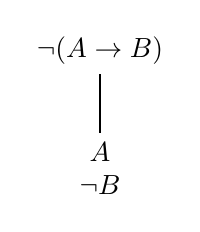
\begin{tikzpicture}[sibling distance=10em,
					every node/.style={align=center}]
					\node{$\neg(A\to B)$}
					child{node{$A$\\$\neg B$}};
					\end{tikzpicture}
				\end{center}
		\end{columns}
		\vspace{7pt}
		\hrule
		\vspace{7pt}
		\begin{columns}
			\column{0.1\textwidth}
				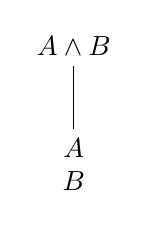
\begin{tikzpicture}[sibling distance=10em,
				every node/.style={align=center}]
				\node{$A\wedge B$}
				child{node{$A$\\$B$}};
				\end{tikzpicture}
			\column{0.35\textwidth}
				\resizebox{\textwidth}{!}{
					\begin{tikzpicture}[sibling distance=10em,
					every node/.style={align=center}]
					\node{$\!\!\!\!\neg(A\wedge B)$}
					child{node{$\neg A$}}
					child{node{$\neg B$}};
					\end{tikzpicture}}
			\column{0.35\textwidth}
				\resizebox{\textwidth}{!}{
					\begin{tikzpicture}[sibling distance=10em,
					every node/.style={align=center}]
					\node{$A\vee B$}
					child{node{$A$}}
					child{node{$B$}};
					\end{tikzpicture}}
			\column{0.12\textwidth}
				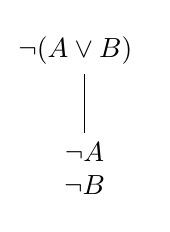
\begin{tikzpicture}[sibling distance=10em,
				every node/.style={align=center}]
				\node{$\!\!\!\!\neg(A\vee B)$}
				child{node{$\neg A$\\$\neg B$}};
				\end{tikzpicture}
		\end{columns}
		\vspace{7pt}
		\hrule
		\vspace{7pt}
		\begin{columns}
			\column{0.35\textwidth}\hspace{-7pt}
				\resizebox{\textwidth}{!}{
					\begin{tikzpicture}[sibling distance=10em,
					every node/.style={align=center}]
					\node{$A\leftrightarrow B$}
					child{node{$A$\\$B$}}
					child{node{$\neg A$\\$\neg B$}};
					\end{tikzpicture}}
			\column{0.35\textwidth}\hspace{-7pt}
				\resizebox{\textwidth}{!}{
					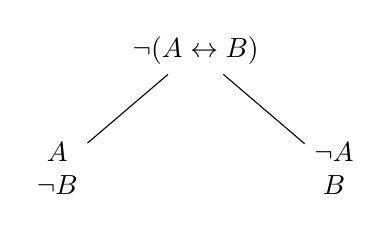
\begin{tikzpicture}[sibling distance=10em,
					every node/.style={align=center}]
					\node{$\neg(A\leftrightarrow B)$}
					child{node{$A$\\$\neg B$}}
					child{node{$\neg A$\\$B$}};
					\end{tikzpicture}}
		\end{columns}
	\[\textcolor{red}{\checkmark}\]
\end{frame}

\begin{frame}\frametitle{Instructions for Tree Construction}
\begin{itemize}
	\item A \emph{literal} is an atomic formula or its negation.
	\item When a non-literal wff has been fully unpacked, check it with $\textcolor{red}{\checkmark}$
\end{itemize}
\begin{enumerate}
	\item Start with premises and the negation of the conclusion.
	\item Inspect each open path for an occurrance of a wff and its negation. If these occur, close the path with $\textcolor{red}{\times}$.
	\item If there is no unchecked non-literal wff on any open path, then stop!
	\item Otherwise, unpack any unchecked non-literal wff on any open path.
	\item Goto \textcircled{\footnotesize 2}.
\end{enumerate}
\begin{itemize}
	\item \emph{Closed branch.} A branch is closed if it contains a wff and its negation.
	\item \emph{Closed tree.} A tree is closed if all its branches are closed.
	\item \emph{Open branch.} A branch is open if it is not closed and no rule can be applied.
	\item \emph{Open tree.} A tree is open if it has at least one open branch.
\end{itemize}
\end{frame}

\begin{frame}\frametitle{Tactics}
\begin{itemize}
	\item Try to apply ``non-branching'' rules first, in order to reduce the number of branches.
	\item Try to close off branches as quickly as possible.
\end{itemize}
\begin{definition}[Deduction]
	$A_1,\dots, A_n\vdash B$ iff there exists a \emph{closed tree} from $\{A_1,\dots, A_n,\neg B\}$.
\end{definition}
\begin{theorem}[Soundness \& Completeness Theorem]
	\[A_1,\dots, A_n\vdash B\iff A_1,\dots, A_n\vDash B\]
\end{theorem}
	\textbf{Remark:} If an inference with propositional formulae is not valid, then its tree will have at least one open branch. The tree method can generate every counterexample of an invalid inference in propositional logic.
\end{frame}

\begin{frame}\frametitle{Examples --- Tree Method}
\begin{flushright}
	\fbox{$p\to q, \neg q\vee r\vdash\neg p\vee r$}
\end{flushright}
	\begin{center}
		\begin{tikzpicture}[sibling distance=10em,
		every node/.style={align=center}]
		\node{\quad$p\to q\;\checkmark$\\
		\;$\neg q\vee r\;\checkmark$\\
		\!\!$\neg(\neg p\vee r)\;\checkmark$}
		child{node{$\neg\neg p$\\$\neg r$}
			child{node{$\neg p$\\$\times$}}
			child{node{$q$}
				child{node{$\neg q$\\$\times$}}
				child{node{$r$\\$\times$}}}};
		\end{tikzpicture}
	\end{center}
\end{frame}

\begin{frame}\frametitle{An open branch corresponds to a valuation}\vspace{-1ex}
\begin{flushright}
	\fbox{$p\vee q, r\vee s, s\to t\stackrel{?}{\vDash} r$}
\end{flushright}
	\begin{center}\vspace{-5ex}
		\begin{tikzpicture}[sibling distance=10em,
		every node/.style={align=center}]
		\node{\;\;\;$p\vee q\;\checkmark$\\
		\;\;\;$r\vee s\;\checkmark$\\
		\;\;\;$s\to t\;\checkmark$\\$\neg r$}
		child{node{$r$\\$\times$}}
		child{node{$s$}
			child{node{$\neg s$\\$\times$}}
			child{node{$t$}
				child{node{$p$}}
				child{node{$q$}}}};
		\end{tikzpicture}
	\end{center}
	\[\nu(r)=0,\quad \nu(s)=1,\quad \nu(t)=1\quad \nu(p)=1\quad\nu(q)=1 \mbox{ or } 0\]
	\[\nu(r)=0,\quad \nu(s)=1,\quad \nu(t)=1\quad \nu(q)=1\quad\nu(p)=1 \mbox{ or } 0\]
	\[\nu\vDash p\vee q,\quad \nu\vDash r\vee s,\quad \nu\vDash s\to t,\quad \nu\nvDash r\]
\end{frame}

\begin{frame}\frametitle{}
\centering
\includegraphics[width=.6\textwidth]{img/fight-math}\\
\textbf{Don't just read it; fight it!}\\
Ask your own questions,\\
look for your own examples,\\
discover your own proofs.\\
Is the hypothesis necessary?\\
Is the converse true?\\
What happens in the classical special case?\\
What about the degenerate cases?\\
Where does the proof use the hypothesis?
\end{frame}

\begin{frame}\frametitle{Exercises --- Tree Method}
		\begin{enumerate}
			\item $p\to(\neg q\to q)\vdash p\to q$
			\item $(p\to r)\wedge(q\to r)\vdash p\vee q\to r$
			\item $(p\to q)\wedge(r\to s)\vdash\neg q\wedge r\to\neg q\wedge s$
			\item $\Big(\big((p\to q)\to(\neg r\to\neg s)\big)\to r\Big)\to t\vdash (t\to p)\to s\to p$
			\item $(p\to q)\vee(q\to r)$
			\item $(p\to q)\to(\neg p\to q)\to q$
			\item $((p\to q)\to p)\to p$
			\item $(p\to q)\wedge(r\to s)\to p\vee r\to q\vee s$
			\item $(p\to q)\wedge r\to\neg(p\wedge r)\vee(q\wedge r)$
			\item $(p\leftrightarrow(p\to q))\to q$
			\item $\neg(p\leftrightarrow q)\leftrightarrow(\neg p\leftrightarrow q)$
		\end{enumerate}
\end{frame}

\begin{frame}\frametitle{Exercises --- Tree Method}
Decide whether the following inferences are valid or not. If not, provide a counterexample.
\begin{enumerate}
	\item $(p\vee q)\wedge r\stackrel{?}{\vDash} p\vee(q\wedge r)$
	\item $p\vee(q\wedge r)\stackrel{?}{\vDash} (p\vee q)\wedge r$
	\item $p\leftrightarrow(q\to r)\stackrel{?}{\vDash}(p\leftrightarrow q)\to r$
	\item $(p\leftrightarrow q)\to r\stackrel{?}{\vDash}p\leftrightarrow(q\to r)$
	\item $\neg(p\to q\wedge r),r\to p\wedge q \stackrel{?}{\vDash}\neg r$
	\item $p\to(q\wedge r), \neg(p\vee q\to r)\stackrel{?}{\vDash}p$
	\item $p\to q, r\to s, p\vee r, \neg(q\wedge s)\stackrel{?}{\vDash}(q\to p)\wedge(s\to r)$
	\item If God does not exist, then it's not the case that \emph{if I pray, my prayers will be answered}; and I don't pray; so God exists.
\end{enumerate}
\end{frame}

%---------------------------------%
\subsection{Meta-Theorems}
%---------------------------------%

\begin{frame}\frametitle{Model \& Semantic Consequence}
\begin{columns}
\column{.42\textwidth}
	\begin{itemize}
		\item $\operatorname{Mod}(A)\coloneqq \left\{\nu: \nu\vDash A\right\}$
		\item $\operatorname{Mod}(\Gamma)\coloneqq \bigcap\limits_{A\in\Gamma}\operatorname{Mod}(A)$
		\item $\operatorname{Th}(\nu)\coloneqq \left\{A: \nu\vDash A\right\}$
		\item $\operatorname{Th}(\mathcal{K})\coloneqq \bigcap\limits_{\nu\in\mathcal{K}}\operatorname{Th}(\nu)$
		\item $\operatorname{Cn}(\Gamma)\coloneqq \left\{A: \Gamma\vDash A\right\}$
	\end{itemize}
\column{.5\textwidth}
	\begin{block}{}
		\begin{itemize}
			\item \textcolor{yellow}{$\Gamma\subset\Gamma'\implies\operatorname{Mod}(\Gamma')\subset\operatorname{Mod}(\Gamma)$}
			\item \textcolor{yellow}{$\mathcal{K}\subset\mathcal{K}'\implies\operatorname{Th}(\mathcal{K}')\subset\operatorname{Th}(\mathcal{K})$}
			\item \textcolor{yellow}{$\Gamma\subset\operatorname{Th}(\operatorname{Mod}(\Gamma))$}
			\item \textcolor{yellow}{$\mathcal{K}\subset\operatorname{Mod}(\operatorname{Th}(\mathcal{K}))$}
			\item $\operatorname{Mod}(\Gamma)=\operatorname{Mod}(\operatorname{Th}(\operatorname{Mod}(\Gamma)))$
			\item $\operatorname{Th}(\mathcal{K})=\operatorname{Th}(\operatorname{Mod}(\operatorname{Th}(\mathcal{K})))$
			\item $\operatorname{Cn}(\Gamma)=\operatorname{Th}(\operatorname{Mod}(\Gamma))$
			\item $\Gamma\subset\Gamma'\implies \operatorname{Cn}(\Gamma)\subset \operatorname{Cn}(\Gamma')$
			\item $\operatorname{Cn}(\operatorname{Cn}(\Gamma))=\operatorname{Cn}(\Gamma)$
		\end{itemize}
	\end{block}
\end{columns}
\end{frame}

\begin{frame}\frametitle{Consistency \& Satisfiability}
	\begin{itemize}
		\item $\Gamma$ is \textcolor{yellow}{consistent} if $\Gamma\nvdash\bot$.
		\item $\Gamma$ is \textcolor{yellow}{Post-consistent} if there is some wff $A:\Gamma\nvdash A$.
		\begin{center}
			\fbox{$\Gamma$ is consistent iff it is Post-consistent.}
		\end{center}
		\item $\Gamma$ is \textcolor{yellow}{maximal} if for every wff $A$, either $A\in\Gamma$ or $\neg A\in\Gamma$.
		\item $\Gamma$ is \textcolor{yellow}{maximal consistent} if it is both consistent and maximal.
	\end{itemize}
	\begin{itemize}
		\item $\Gamma$ is \textcolor{yellow}{satisfiable} if $\operatorname{Mod}(\Gamma)\neq\emptyset$.
		\item $\Gamma$ is \textcolor{yellow}{finitely satisfiable} if every finite subset of $\Gamma$ is satisfiable.
	\end{itemize}
	\begin{block}{}
		\begin{itemize}
			\item If $\Gamma$ is consistent and $\Gamma\vdash A$, then $\Gamma\cup\{A\}$ is consistent.
			\item $\Gamma\cup\{\neg A\}$ is inconsistent iff $\Gamma\vdash A$.
			\item {\small If $\Gamma$ is maximal consistent, then $A\notin\Gamma\implies\Gamma\cup\{A\}\;\text{is inconsistent}$.}
		\end{itemize}
	\end{block}
\end{frame}

\begin{frame}\frametitle{Soundness Theorem}
	\begin{theorem}[Soundness Theorem]
		\[\Gamma\vdash A\implies\Gamma\vDash A\]
	\end{theorem}
	\begin{proof}
		Prove by induction on the length of the deduction sequence.\\
		Case1: $A$ is an axiom. (truth table)\\
		Case2: $A\in\Gamma$\\
		Case3:
		\[\left.
		\begin{aligned}
		\Gamma&\vDash C_j\\
		\Gamma&\vDash C_j\to A
		\end{aligned}\right\}\implies\Gamma\vDash A\]
	\end{proof}
	\begin{corollary}
		Any \textcolor{yellow}{satisfiable} set of wffs is \textcolor{yellow}{consistent}.
	\end{corollary}
\end{frame}

\begin{frame}\frametitle{Compactness Theorem}
\setlength\abovedisplayskip{0pt}
\setlength\belowdisplayskip{0pt}
	\begin{theorem}[Compactness Theorem]
		A set of wffs is satisfiable iff it is finitely satisfiable.
	\end{theorem}
	\begin{block}{}
	如果语言可以说无穷析取,则没有紧致性。$\left\{\bigvee\limits_{i=1}^\infty p_i,\neg p_1,\neg p_2,\dots\right\}$
	\end{block}
	\begin{corollary}
		If $\Gamma\vDash A$, then there is a finite $\Gamma_0\subset\Gamma$ s.t. $\Gamma_0\vDash A$.
	\end{corollary}
	\begin{proof}
		\begin{align*}
		\Gamma_0\nvDash A\;\text{for any}\;\Gamma_0\subset\Gamma&\implies\Gamma_0\cup\{\neg A\}\;\text{is satisfiable for any}\;\Gamma_0\subset\Gamma\\
		&\implies\Gamma\cup\{\neg A\}\;\text{is satisfiable}\\
		&\implies\Gamma\nvDash A
		\end{align*}
	\end{proof}
\end{frame}

\begin{frame}\frametitle{Applications of Compactness}
	\begin{figure}
	\includegraphics[width=.9\textwidth]{img/4color}
	\end{figure}
	\begin{center}
		\resizebox{\textwidth}{!}{\fbox{An infinite graph $(V,E)$ is $n$-colorable iff every finite subgraph of $(V,E)$ is $n$-colorable.}}
	\end{center}
\begin{proof}
Take $\left\{p_v^i: v\in V, 1\leq i\leq n\right\}$ as the set of atoms.\\
$\Gamma\coloneqq \left\{p_v^1\vee\dots\vee p_v^n: v\in V\right\}\cup\left\{\neg\big(p_v^i\wedge p_v^j\big): v\in V, 1\leq i<j\leq n\right\}\cup\left\{\neg\big(p_v^i\wedge p_w^i\big): (v,w)\in E, 1\leq i\leq n\right\}$
\end{proof}
\end{frame}

\begin{frame}\frametitle{Completeness Theorem --- Post1921}
		\begin{theorem}[Completeness Theorem]
			\[\Gamma\vDash A\implies\Gamma\vdash A\]
		\end{theorem}
		\begin{corollary}
			Any \textcolor{yellow}{consistent} set of wffs is \textcolor{yellow}{satisfiable}.
		\end{corollary}\vspace*{-3ex}
			{\Large \[\arraycolsep=0.7pt\def\arraystretch{1.7}
					\begin{array}{cccc}
					&\Gamma\vDash A&\iff&\Gamma\vdash A\\
					&\rotatebox[origin=C]{90}{$\iff$}&&\rotatebox[origin=C]{90}{$\iff$}\\
					&\Gamma\cup\{\neg A\}\atop{\text{unsatisfiable}}&\iff&\Gamma\cup\{\neg A\}\atop{\text{inconsistent}}
					\end{array}
					\]}
		\begin{corollary}[Compactness Theorem]
			A set of wffs is satisfiable iff it is finitely satisfiable.
		\end{corollary}
\end{frame}

\begin{frame}\frametitle{Proof of Completeness Theorem}
	\begin{proof}
		step$1$. Extend the consistent set $\Gamma$ to a maximal consistent set $\Delta$.\\
		Let $\left\langle A_i: i\in\mathbb{N}\right\rangle$ be a fixed enumeration of the wffs.
		\begin{align*}
		\Delta_0&\coloneqq \Gamma\\
		\Delta_{n+1}&\coloneqq 
		\begin{cases}
		\Delta_n\cup\{A_n\} &\text{if $\Delta_n\cup\{A_n\}$ is consistent}\\
		\Delta_n\cup\{\neg A_n\} &\text{otherwise}
		\end{cases}\\
		\Delta&\coloneqq \bigcup\limits_{n\in\mathbb{N}}\Delta_n
		\end{align*}
		step$2$. Define a truth assignment that satisfies $\Gamma$.
		\[\nu(p)\coloneqq 
		\begin{cases}
		1 &\text{if}\; p\in\Delta\\
		0 &\text{otherwise}
		\end{cases}\implies\big(\nu\vDash A\iff A\in\Delta\big)\]
	\end{proof}
\end{frame}

\begin{frame}\frametitle{Decidability --- Post1921}
	\begin{theorem}
		There is an effective procedure that, given any expression, will decide whether or not it is a wff.
	\end{theorem}
	\begin{theorem}
		There is an effective procedure that, given a finite set $\Gamma\cup\{A\}$ of wffs, will decide whether or not $\Gamma\vDash A$.
	\end{theorem}
	\begin{theorem}
		If $\Gamma$ is a decidable set of wffs, then the set of logical consequences of $\Gamma$ is recursively enumerable.
	\end{theorem}
\end{frame}

\begin{frame}\frametitle{Post 1897-1954}
\begin{columns}
\column{.4\textwidth}
\begin{figure}
	\includegraphics[height=.9\textwidth,angle=0,origin=c]{img/post}
\end{figure}
\column{.6\textwidth}
\begin{itemize}
	\item Truth table
	\item Completeness of propositional logic
	\item Post machine
	\item Post canonical system
	\item Post correspondence problem
	\item Post problem
\end{itemize}
\end{columns}
\end{frame}

\begin{frame}\frametitle{Theory \& Axiomatization}
	\begin{block}{}
		\centering\textcolor{red}{What is ``theory''?}
	\end{block}
	\begin{itemize}
		\item A set $\Gamma$ of sentences is a \textcolor{yellow}{theory} if $\Gamma=\operatorname{Cn}(\Gamma)$.
		\item A theory $\Gamma$ is \textcolor{yellow}{complete} if for every sentence $A$, either $A\in\Gamma$ or $\neg A\in\Gamma$.
		\item A theory $\Gamma$ is \textcolor{yellow}{axiomatizable} if there is a decidable set $\Sigma$ of sentences s.t. $\Gamma=\operatorname{Cn}(\Sigma)$.
		\item A theory $\Gamma$ is \textcolor{yellow}{finitely axiomatizable} if $\Gamma=\operatorname{Cn}(\Sigma)$ for some finite set $\Sigma$ of sentences.
	\end{itemize}
\end{frame}

\begin{frame}\frametitle{\small Model Checking \& Satisfiability Checking \& Validity Checking\footnote{\tiny \href{https://www.scottaaronson.com/papers/philos.pdf}{Aaronson: Why philosophers should care about computational complexity.}}}
	\begin{itemize}
		\item Given a model $\nu$ and a formula $A$. Is $\nu\vDash A$?\hfill ---\textcolor{yellow}{P}
		\item Given a formula $A$. Is there a model $\nu$ s.t. $\nu\vDash A$?\hfill ---\textcolor{yellow}{NP}
		\item Given a sentence $A$. Is $\vDash A$?
	\end{itemize}
\begin{minipage}{\textwidth}
	\begin{columns}
		\column{0.28\textwidth}
			\begin{figure}
				\includegraphics[width=\textwidth]{img/euler-bridge}\\
				\includegraphics[width=\textwidth]{img/eulerian-path}\caption{\tiny{\textit{Eulerian Circle(P)}}}
			\end{figure}
		\column{0.3\textwidth}\vspace{-0.3cm}
			\begin{figure}
				\includegraphics[width=0.7\textwidth]{img/hamiltonian-path}\vspace{-0.2cm}\caption{\tiny{\textit{Hamiltonian Circle(NPC)}}}\vspace{-0.2cm}
				\includegraphics[width=0.7\textwidth]{img/graph-coloring}\vspace{-0.3cm}\caption{\tiny{\textit{Graph Coloring(NPC)}}}
			\end{figure}
		\column{0.4\textwidth}\vspace{-0.5cm}
			\begin{center}
				\begin{figure}
					\includegraphics[width=\textwidth]{img/hanoi.pdf}
				\end{figure}
			\end{center}
	\end{columns}
\end{minipage}
\end{frame}

%%%%%%%%%%%%%%%%%%%%%%%%%%%%%%
\subsection{Application}
%%%%%%%%%%%%%%%%%%%%%%%%%%%%%%

\begin{frame}\frametitle{Party and Friends}
	\begin{problem}
		\begin{itemize}
			\item We want to throw a party for \textcolor{yellow}{Tweety}, \textcolor{yellow}{Gentoo} and \textcolor{yellow}{Tux}.
			\item But they have different circles of friends and dislike some.
			\item Tweety tells you that he would like to see \emph{either} his friend \textcolor{yellow}{Kimmy} \emph{or} not to meet Gentoo's \textcolor{yellow}{Alice}, but not both.
			\item But Gentoo proposes to invite \textcolor{yellow}{Alice} or \textcolor{yellow}{Harry} or both.
			\item Tux, however, does not like \textcolor{yellow}{Harry} and \textcolor{yellow}{Kimmy} too much, so he suggests to \textcolor{yellow}{exclude} at least one of them.
		\end{itemize}
	\end{problem}\pause
	\begin{solution}
		\[(K\vee\neg A)\wedge\neg(K\wedge\neg A)\wedge(A\vee H)\wedge(\neg H\vee\neg K)\]
	\end{solution}
\end{frame}

\begin{frame}\frametitle{Sudoku}
\begin{columns}
\column{.37\textwidth}
\begin{center}
\resizebox{\textwidth}{!}{$
\begin{array}{!{\vrule width2pt}c|c|c!{\vrule width2pt}c|c|c!{\vrule width2pt}c|c|c!{\vrule width2pt}}
\Xhline{2pt}
&&&&&&&&\\
\hline
&\textcolor{red}{\mathbf{8}}&\textcolor{red}{\mathbf{6}}&&&&\textcolor{red}{\mathbf{2}}&\textcolor{red}{\mathbf{9}}&\\
\hline
\textcolor{red}{\mathbf{4}}&&&\textcolor{red}{\mathbf{1}}&&\textcolor{red}{\mathbf{5}}&&&\textcolor{red}{\mathbf{8}}\\
\Xhline{2pt}
\textcolor{red}{\mathbf{7}}&&&&\textcolor{red}{\mathbf{9}}&&&&\textcolor{red}{\mathbf{4}}\\
\hline
\textcolor{red}{\mathbf{1}}&&&&&&&&\textcolor{red}{\mathbf{9}}\\
\hline
&\textcolor{red}{\mathbf{5}}&&&&&&\textcolor{red}{\mathbf{1}}&\\
\Xhline{2pt}
&&\textcolor{red}{\mathbf{8}}&&&&\textcolor{red}{\mathbf{3}}&&\\
\hline
&&&\textcolor{red}{\mathbf{5}}&&\textcolor{red}{\mathbf{9}}&&&\\
\hline
&&&&\textcolor{red}{\mathbf{2}}&&&&\\
\Xhline{2pt}
\end{array}
$}
\end{center}
\centering\textcolor{yellow}{$p(i,j,n)\coloneqq $ the cell in row $i$ and column $j$ contains the number $n$}
\column{.63\textwidth}
\begin{itemize}
				\item Every row/column contains every number.
				\[\bigwedge\limits_{i=1}^9\bigwedge\limits_{n=1}^9\bigvee\limits_{j=1}^9 p(i,j,n)\qquad\bigwedge\limits_{j=1}^9\bigwedge\limits_{n=1}^9\bigvee\limits_{i=1}^9 p(i,j,n)\]
				\item Every $3\times3$ block contains every number.
				\[\bigwedge\limits_{r=0}^2\bigwedge\limits_{s=0}^2\bigwedge\limits_{n=1}^9\bigvee\limits_{i=1}^3\bigvee\limits_{j=1}^3 p(3r+i,3s+j,n)\]
				\item No cell contains more than one number.
				
				for all $1\leq i,j,n,n'\leq 9$ and $n\neq n'$: \[p(i,j,n)\to\neg p(i,j,n')\]
\end{itemize}
\end{columns}
\end{frame}

\begin{frame}\frametitle{Shannon --- Digital Circuit Design}
	\begin{figure}[!htbp]
		\begin{center}
			\includegraphics[width=0.8\textwidth,angle=0,origin=c]{img/circuit1}
		\end{center}
	\end{figure}
	\[(A\wedge B)\vee((C\vee A)\wedge\neg B)\semeq A\vee(C\wedge\neg B)\]
	\begin{figure}[!htbp]
		\begin{center}
			\includegraphics[width=0.8\textwidth,angle=0,origin=c]{img/circuit2}
		\end{center}
	\end{figure}
\end{frame}

\begin{frame}\frametitle{Shannon --- Digital Circuit Design}
\begin{figure}
\includegraphics[width=.9\textwidth]{img/boole-circuit.pdf}
\end{figure}
\[(A\vee\neg C)\wedge(B\vee\neg C)\semeq(A\wedge B)\vee\neg C\]
\end{frame}

\begin{frame}\frametitle{McCulloch-Pitts Artificial Neural Network}
	\begin{columns}\hspace{-1cm}
		\column{.6\textwidth}
			\resizebox{\textwidth}{!}{
				\begin{minipage}{\textwidth}
					\begin{tikzpicture}
					\node[rectangle, red, ultra thick, fill=green!50!darkgray, opacity=1,label=above:{\parbox{2cm}{\centering activation\\ function}}] at (2,-2) (sigmoid) {\huge $g$};
					\node[green,label=above:{\parbox{2cm}{\centering output}}] at (4,-2) (output) {$y$};
					%%Create a style for the arrows we are using
					\tikzset{normal arrow/.style={draw,-triangle 45,very thick}}
					%%Create the different coordinates to place the nodes
					\path (0,0) coordinate (1) ++(0,-2) coordinate (2) ++(0,-2) coordinate (3);
					\path (1) ++(-2,-1) coordinate (x1);
					\path (3) ++(-2,1) coordinate (x2);
					%%Place nodes at each point using the foreach construct
					\node[draw,circle,shading=axis,top color=green!50!darkgray, bottom color=green,shading angle=5] at (2) (n2) {$\sum$};
					\node[above of=n2,above=.5cm,label=above:{\parbox{2cm}{\centering bias}}] (b) {$1$};
					\node[below of=n2,below=1ex] {linear};
					\node[below of=sigmoid,below=1ex] {nonlinear};
					\node[left of=n2,left=.2cm] (vdots) {\textcolor{green!50!yellow}{\huge $\vdots$}};
					%%Place the remaining nodes separately
					\node[label=above:{\parbox{2cm}{$\;\,$ inputs}}] (nx1) at (x1) {$x_1$};
					\node (nx2) at (x2) {$x_n$};
					%\node (ny) at (7) {$y$};
					\path[normal arrow,green!50!yellow] (b) -- node[right=.05em,green!50!yellow] {$b$} (n2);
					\path[normal arrow,green!50!yellow] (n2) -- (sigmoid);
					\path[normal arrow,green!50!yellow] (sigmoid) -- (output);
					\path[normal arrow,green!50!yellow] (nx1) -- node[label=above:{\parbox{2cm}{\centering\small weights}}][above=.3em,green!50!yellow](w1) {$w_1$} (n2);
					\path[normal arrow,green!50!yellow] (nx2) -- node[below=.3em,green!50!yellow] {$w_n$} (n2);
					\end{tikzpicture}
			\end{minipage}}
			{\Large \[y=g\left(\sum\limits_{i=1}^n w_ix_i+b\right)\]}
		\column{.4\textwidth}
			\resizebox{.8\textwidth}{!}{
				\begin{minipage}{\textwidth}
					\begin{tikzpicture}
					\node[red, rectangle, fill=green!50!darkgray, opacity=1] at (2,-2) (sigmoid) {$\chi_{\geq 0}$};
					\node[green] at (4,-2) (and) {\Huge{$\wedge$}};
					%%Create a style for the arrows we are using
					\tikzset{normal arrow/.style={draw,-triangle 45,very thick}}
					%%Create the different coordinates to place the nodes
					\path (0,0) coordinate (1) ++(0,-2) coordinate (2) ++(0,-2) coordinate (3);
					\path (1) ++(-2,-1) coordinate (x1);
					\path (3) ++(-2,1) coordinate (x2);
					%%Place nodes at each point using the foreach construct
					\node[draw,circle,shading=axis,top color=green!50!darkgray, bottom color=green,shading angle=5] at (2) (n2) {$\sum$};
					\node[above of=n2,above=.5cm] (b) {$1$};
					%%Place the remaining nodes separately
					\node (nx1) at (x1) {$x_1$};
					\node (nx2) at (x2) {$x_2$};
					%\node (ny) at (7) {$y$};
					\path[normal arrow,green!50!yellow] (b) -- node[right=.05em,green!50!yellow] {$-2$} (n2);
					\path[normal arrow,green!50!yellow] (n2) -- (sigmoid);
					\path[normal arrow,green!50!yellow] (sigmoid) -- (and);
					\path[normal arrow,green!50!yellow] (nx1) -- node[above=.5em,green!50!yellow] {$+1$} (n2);
					\path[normal arrow,green!50!yellow] (nx2) -- node[below=.5em,green!50!yellow] {$+1$} (n2);
					\end{tikzpicture}
			\end{minipage}}\\
			\resizebox{.8\textwidth}{!}{
				\begin{minipage}{\textwidth}\vspace{-.5cm}
					\begin{tikzpicture}
					\node[red, rectangle, fill=green!50!darkgray, opacity=1] at (2,-2) (sigmoid) {$\chi_{\geq 0}$};
					\node[green] at (4,-2) (or) {\Huge{$\vee$}};
					%%Create a style for the arrows we are using
					\tikzset{normal arrow/.style={draw,-triangle 45,very thick}}
					%%Create the different coordinates to place the nodes
					\path (0,0) coordinate (1) ++(0,-2) coordinate (2) ++(0,-2) coordinate (3);
					\path (1) ++(-2,-1) coordinate (x1);
					\path (3) ++(-2,1) coordinate (x2);
					\node[draw,circle,shading=axis,top color=green!50!darkgray, bottom color=green,shading angle=5] at (2) (n2) {$\sum$};
					\node[above of=n2,above=.5cm] (b) {$1$};
					%%Place the remaining nodes separately
					\node (nx1) at (x1) {$x_1$};
					\node (nx2) at (x2) {$x_2$};
					%\node (ny) at (7) {$y$};
					\path[normal arrow,green!50!yellow] (b) -- node[right=.05em,green!50!yellow] {$-1$} (n2);
					\path[normal arrow,green!50!yellow] (n2) -- (sigmoid);
					\path[normal arrow,green!50!yellow] (sigmoid) -- (or);
					\path[normal arrow,green!50!yellow] (nx1) -- node[above=.5em,green!50!yellow] {$+1$} (n2);
					\path[normal arrow,green!50!yellow] (nx2) -- node[below=.5em,green!50!yellow] {$+1$} (n2);
					\end{tikzpicture}
			\end{minipage}}\\
			\resizebox{.8\textwidth}{!}{
				\begin{minipage}{\textwidth}\vspace{-.5cm}
					\begin{tikzpicture}
					\node[red, rectangle, fill=green!50!darkgray, opacity=1] at (2,-2) (sigmoid) {$\chi_{\geq 0}$};
					\node[green] at (4,-2) (not) {\Huge{$\neg$}};
					%%Create a style for the arrows we are using
					\tikzset{normal arrow/.style={draw,-triangle 45,very thick}}
					%%Create the different coordinates to place the nodes
					\path (0,0) coordinate (1) ++(0,-2) coordinate (2) ++(0,-2) coordinate (3);
					\path (1) ++(-2,-2) coordinate (x1);
					%%Place nodes at each point using the foreach construct
					\node[draw,circle,shading=axis,top color=green!50!darkgray, bottom color=green,shading angle=5] at (2) (n2) {$\sum$};
					\node[above of=n2,above=.5cm] (b) {$1$};
					%%Place the remaining nodes separately
					\node (nx1) at (x1) {$x$};
					%\node (ny) at (7) {$y$};
					\path[normal arrow,green!50!yellow] (b) -- node[right=.05em,green!50!yellow] {$0$} (n2);
					\path[normal arrow,green!50!yellow] (n2) -- (sigmoid);
					\path[normal arrow,green!50!yellow] (sigmoid) -- (not);
					\path[normal arrow,green!50!yellow] (nx1) -- node[above=.5em,green!50!yellow] {$-1$} (n2);
					\end{tikzpicture}
			\end{minipage}}
	\end{columns}
\end{frame}

\begin{frame}\frametitle{}
\begin{block}{《三体》}
\begin{itemize}
	\item 秦始皇:朕当然需要预测太阳的运行,但你们让我集结三千万大军,至少要首先向朕演示一下这种计算如何进行吧。
	\item 冯诺依曼:陛下,请给我三个士兵,我将为您演示。……
	\item 秦始皇:他们不需要学更多的东西了吗?
	\item 冯诺依曼:不需要,我们组建一千万个这样的门部件,再将这些部件组合成一个系统,这个系统就能进行我们所需要的运算,解出那些预测太阳运行的微分方程。
\end{itemize}
\end{block}
\begin{columns}	
\column{0.3\textwidth}
\[\begin{tabu}{cc|c}
	\hline
	p & q & p\oplus q\\
	\hline
	0 & 0 & 0\\
	0 & 1 & 1\\
	1 & 0 & 1\\
	1 & 1 & 0\\
	\hline
\end{tabu}\]
\column{0.4\textwidth}
\begin{align*}
w_1\cdot 0+w_2\cdot 0+b<0\\
w_1\cdot 0+w_2\cdot 1+b\geq 0\\
w_1\cdot 1+w_2\cdot 0+b\geq 0\\
w_1\cdot 1+w_2\cdot 1+b<0
\end{align*}
\column{0.3\textwidth}
\begin{align*}
b<0\\
w_2+b\geq 0\\
w_1+b\geq 0\\
w_1+w_2+b<0
\end{align*}
\end{columns}\vspace*{7pt}
A simple single-layer perception can't solve nonlinearly separable problems.
\end{frame}

\begin{frame}\frametitle{Finite State Automaton}
\begin{columns}
\column{.5\textwidth}
\begin{figure}[H]
\includegraphics[width=\textwidth]{img/boole-automata.pdf}
\end{figure}
\column{.5\textwidth}
\[
\begin{tabu}{ccc|cc}
\hline
y_1&y_2&x&y_1^+&y_2^+\\
\hline
0 & 0 & 0 & 1 & 0\\
0 & 0 & 1 & 1 & 0\\
0 & 1 & 0 & 0 & 0\\
0 & 1 & 1 & 0 & 0\\
1 & 0 & 0 & 1 & 1\\
1 & 0 & 1 & 0 & 1\\
1 & 1 & 0 & 0 & 0\\
1 & 1 & 1 & 0 & 1\\
\hline
\end{tabu}
\]
\end{columns}
\begin{align*}
y_1^+&=\bar{y}_1\bar{y}_2+\bar{x}\bar{y}_2\\
y_2^+&=y_1\bar{y}_2+xy_1
\end{align*}
\end{frame}

\begin{frame}\frametitle{Reversible Computing --- Fredkin Gate: $\operatorname{CSWAP}$}
\begin{columns}
\column{.38\textwidth}
\[
\begin{tabu}{lll|lll}
\hline
c & p & q & x & y & z\\
\hline
0 & 0 & 0 & 0 & 0 & 0\\
0 & 0 & 1 & 0 & 0 & 1\\
0 & 1 & 0 & 0 & 1 & 0\\
0 & 1 & 1 & 0 & 1 & 1\\
1 & 0 & 0 & 1 & 0 & 0\\
1 & 0 & 1 & 1 & 1 & 0\\
1 & 1 & 0 & 1 & 0 & 1\\
1 & 1 & 1 & 1 & 1 & 1\\
\hline
\end{tabu}\]
\column{.45\textwidth}
\begin{figure}[H]
\includegraphics[width=.8\textwidth]{img/fredkin-gate.pdf}\caption{transmit the first bit unchanged and swap the last two bits iff the first bit is $1$. $f:(c,p,q)\mapsto(c,c\cdot q+\overline{c}\cdot p,c\cdot p+\overline{c}\cdot q)$}
\end{figure}
\end{columns}
\[\tiny\operatorname{CSWAP}=
\begin{bmatrix}
1 & 0 & 0 & 0 & 0 & 0 & 0 & 0 \\
0 & 1 & 0 & 0 & 0 & 0 & 0 & 0 \\
0 & 0 & 1 & 0 & 0 & 0 & 0 & 0 \\
0 & 0 & 0 & 1 & 0 & 0 & 0 & 0 \\
0 & 0 & 0 & 0 & 1 & 0 & 0 & 0 \\
0 & 0 & 0 & 0 & 0 & 0 & 1 & 0 \\
0 & 0 & 0 & 0 & 0 & 1 & 0 & 0 \\
0 & 0 & 0 & 0 & 0 & 0 & 0 & 1 \\
\end{bmatrix}
\]
\begin{description}
\item[\textcolor{red}{$\neg$}] $p=0\;\;\&\;\;q=1\implies z=\overline{c}$
\item[\textcolor{red}{$\wedge$}] $q=0\implies z=c\cdot p$
\end{description}
\end{frame}

\begin{frame}\frametitle{Exercise}
\begin{block}{宝藏在哪里?}
你面前有三扇门,只有一扇门后是宝藏。门上各有一句话,只有一扇门上的是真话。
\begin{enumerate}
	\item 宝藏不在这儿。
	\item 宝藏不在这儿。
	\item 宝藏在\textcircled{\footnotesize 2}号门。
\end{enumerate}
\end{block}
\begin{itemize}
	\item \textcircled{\footnotesize 1} $\neg t_1$; \textcircled{\footnotesize 2} $\neg t_2$; \textcircled{\footnotesize 3} $t_2$.
	\item 只有一扇门上的是真话。
	$(\neg t_1\wedge\neg\neg t_2\wedge\neg t_2)\vee(\neg\neg t_1\wedge\neg t_2\wedge\neg t_2)\vee(\neg\neg t_1\wedge\neg\neg t_2\wedge t_2)$
	\item 只有一扇门后是宝藏。\\
	$(t_1\wedge\neg t_2\wedge\neg t_3)\vee(\neg t_1\wedge t_2\wedge\neg t_3)\vee(\neg t_1\wedge\neg t_2\wedge t_3)$
\end{itemize}
\end{frame}

\begin{frame}\frametitle{Exercise}
		\begin{block}{谁是凶手?}
			一起凶杀案有三个嫌疑人:小白、大黄和老王。
			\begin{enumerate}
				\item 至少有一人是凶手,但不可能三人同时犯罪。
				\item 如果小白是凶手,那么老王是同犯。
				\item 如果大黄不是凶手,那么老王也不是。
			\end{enumerate}
		\end{block}
		\begin{block}{谁是窃贼?}
			\begin{enumerate}
				\item 钱要么是甲偷的要么是乙偷的。
				\item 如果是甲偷的,则偷窃时间不会在午夜前。
				\item 如果乙的证词正确,则午夜时灯光未灭。
				\item 如果乙的证词不正确,则偷窃发生在午夜前。
				\item 午夜时没有灯光。
			\end{enumerate}
		\end{block}
\end{frame}

\begin{frame}\frametitle{Exercise}
		\begin{block}{哪个部落的?}
		一个岛上有T、F两个部落,T部落的居民只说真话,F部落的居民只说谎。你在岛上遇到了小白、大黄、老王三个土著。
			\begin{enumerate}
				\item 小白:“如果老王说谎,我或大黄说的就是真话”。
				\item 大黄:“只要小白或老王说真话,那么,我们三人中有且只有一人说真话是不可能的”。
				\item 老王:“小白或大黄说谎当且仅当小白或我说真话”。
			\end{enumerate}
		\end{block}
		\begin{block}{我在做什么?}
			\begin{enumerate}
				\item 如果我不在打网球,那就在看网球。
				\item 如果我不在看网球,那就在读网球杂志。
				\item 但我不能同时做两件以上的事。
			\end{enumerate}
		\end{block}
\end{frame}

%%%%%%%%%%%%%%%%%%%%
\subsection{Boolean Algebra}
%%%%%%%%%%%%%%%%%%%%

\begin{frame}\frametitle{Logic as Algebra --- Boolean Algebra $\mathrm{BA}$}
\begin{columns}[onlytextwidth]
\column{0.5\textwidth}
Boolean Algebra $\mathscr{L}=\{0,1,+,\cdot,\overline{\phantom{x}}\}$
			\begin{itemize}
				\item \textcolor{green}{$x+(y+z)=(x+y)+z$}\\
				\textcolor{green}{$x\cdot(y\cdot z)=(x\cdot y)\cdot z$}
				\item \textcolor{green}{$x+y=y+x\quad x\cdot y=y\cdot x$}
				\item \textcolor{green}{$x+(x\cdot y)=x\quad x\cdot(x+y)=x$}
				\item $x+(y\cdot z)=(x+y)\cdot(x+z)$\\
				$x\cdot(y+z)=(x\cdot y)+(x\cdot z)$
				\item $\overline{\overline{x}}=x$
				\item $\overline{x+y}=\overline{x}\cdot\overline{y}\quad\overline{x\cdot y}=\overline{x}+\overline{y}$
				\item $x+\overline{x}=1\quad x\cdot\overline{x}=0\quad 0\neq 1$
				\item $x+0=x\quad x\cdot 0=0$
				$x+1=1\quad x\cdot 1=x$
			\end{itemize}
\column{0.5\textwidth}
			\[\text{\textcolor{yellow}{Logic}}\]
			\vspace{-17pt}
			\resizebox{\textwidth}{!}{
				\xymatrix{\text{proposition} \ar[d]_{\text{translate}} \ar[r]^{\text{deduce}} & \text{proposition}\\
					\text{equation} \ar[r]^{\text{calculate}} & \text{equation} \ar[u]_{\text{translate}}}
			}\vspace{-10pt}
			\[\text{\textcolor{yellow}{Algebra}}\]
	\end{columns}
\end{frame}

\begin{frame}\frametitle{Power Set Algebra}
\[(\operatorname{P}(A),\emptyset,A,\cup,\cap,\overline{\phantom{x}})\]
\centering
\setlength{\unitlength}{0.42pt}
\begin{picture}(240,240)
\put(10,80){$X$}
\put(205,80){$Y$}
\put(0,0){\line(1,0){240}}
\put(0,0){\line(0,1){180}}
\put(0,180){\line(1,0){240}}
\put(240,0){\line(0,1){180}}
\put(90,90){\circle{100}}
\put(150,90){\circle{100}}
\put(40,90){\line(1,0){160}}
\put(45,110){\line(1,0){150}}
\put(45,70){\line(1,0){150}}
\put(60,130){\line(1,0){120}}
\put(60,50){\line(1,0){120}}
\end{picture}
\begin{picture}(240,240)
\put(45,80){$X$}
\put(170,80){$Y$}
\put(0,0){\line(1,0){240}}
\put(0,0){\line(0,1){180}}
\put(0,180){\line(1,0){240}}
\put(240,0){\line(0,1){180}}
\put(90,90){\circle{100}}
\put(150,90){\circle{100}}
\put(100,90){\line(1,0){40}}
\put(105,110){\line(1,0){30}}
\put(105,70){\line(1,0){30}}
\end{picture}
\begin{picture}(180,240)
\put(45,80){$X$}
\put(0,0){\line(1,0){180}}
\put(0,0){\line(0,1){180}}
\put(0,180){\line(1,0){180}}
\put(180,0){\line(0,1){180}}
\put(90,90){\circle{100}}
\put(0,90){\line(1,0){40}}
\put(140,90){\line(1,0){40}}
\put(0,110){\line(1,0){45}}
\put(135,110){\line(1,0){45}}
\put(0,70){\line(1,0){45}}
\put(135,70){\line(1,0){45}}
\put(0,130){\line(1,0){60}}
\put(120,130){\line(1,0){60}}
\put(0,50){\line(1,0){60}}
\put(120,50){\line(1,0){60}}
\put(0,150){\line(1,0){180}}
\put(0,30){\line(1,0){180}}
\put(0,170){\line(1,0){180}}
\put(0,10){\line(1,0){180}}
\end{picture}
\begin{columns}
\column{.5\textwidth}
\[x\oplus y\coloneqq (x\cdot\overline{y})+(\overline{x}\cdot y)\]
\[x=y\iff x\oplus y=0\]
\column{.5\textwidth}
\setlength{\unitlength}{0.42pt}
\begin{picture}(240,240)
\put(10,80){$X$}
\put(205,80){$Y$}
\put(0,0){\line(1,0){240}}
\put(0,0){\line(0,1){180}}
\put(0,180){\line(1,0){240}}
\put(240,0){\line(0,1){180}}
\put(90,90){\circle{100}}
\put(150,90){\circle{100}}
\put(40,90){\line(1,0){60}}
\put(140,90){\line(1,0){60}}
\put(45,110){\line(1,0){60}}
\put(135,110){\line(1,0){60}}
\put(45,70){\line(1,0){60}}
\put(135,70){\line(1,0){60}}
\put(60,130){\line(1,0){120}}
\put(60,50){\line(1,0){120}}
\end{picture}
\end{columns}
\end{frame}

\begin{frame}\frametitle{Propositional Logic vs Boolean Algebra}
\setlength\abovedisplayskip{0pt}
\setlength\abovedisplayskip{0pt}
	\begin{columns}
		\column{0.5\textwidth}
			\begin{align*}
			(\bot)^*&\coloneqq 0\\
			(\top)^*&\coloneqq 1\\
			(p)^*&\coloneqq p\\
			(\neg A)^*&\coloneqq \overline{A^*}\\
			(A\vee B)^*&\coloneqq A^*+B^*\\
			(A\wedge B)^*&\coloneqq A^*\cdot B^*
			\end{align*}
		\column{0.5\textwidth}
			\begin{align*}
			(0)'&\coloneqq \bot\\
			(1)'&\coloneqq \top\\
			(p)'&\coloneqq p\\
			\left(\overline{A}\right)'&\coloneqq \neg A'\\
			(A+B)'&\coloneqq A'\vee B'\\
			(A\cdot B)'&\coloneqq A'\wedge B'
			\end{align*}
	\end{columns}
\begin{columns}
\column{0.45\textwidth}
\begin{block}{}
	\[A\vdash B\iff\mathrm{BA}\vdash A^*\leq B^*\]
\end{block}
\column{0.45\textwidth}
\begin{block}{}
	\[\mathrm{BA}\vdash A\leq B\iff A'\vdash B'\]
\end{block}
\end{columns}
	\[\text{where}\; x\leq y\coloneqq x\cdot\overline{y}=0\]
\end{frame}

\begin{frame}\frametitle{Boolean Algebra vs Propositional Logic}
	\begin{block}{Exercise}
		Alice, Ben, Charlie, and Diane are considering going to a
		Halloween party.
		\begin{enumerate}
			\item If Alice goes then Ben won't go and Charlie will.
			\item If Ben and Diane go, then either Alice or Charlie (but not both) will go.
			\item If Charlie goes and Ben does not, then Diane will go but Alice will not.
		\end{enumerate}
	\end{block}
	\begin{align*}
	A&\to\neg B\wedge C &\textcolor{yellow}{A\cdot(B+\overline{C})}&\textcolor{yellow}{=0}\\
	B\wedge D&\to(A\wedge\neg C)\vee(\neg A\wedge C) &\textcolor{yellow}{B\cdot D\cdot(\overline{A}\cdot\overline{C}+A\cdot C)}&\textcolor{yellow}{=0}\\
	\neg B\wedge C&\to\neg A\wedge D &\textcolor{yellow}{\overline{B}\cdot C\cdot(A+\overline{D})}&\textcolor{yellow}{=0}
	\end{align*}
\end{frame}

\begin{frame}\frametitle{怎么得大奖?}
	\begin{problem}[怎么得大奖?]
		\begin{itemize}
			\item 说真话得一个大奖或一个小奖。
			\item 说假话不得奖。
		\end{itemize}
	\end{problem}
\begin{itemize}
\item b: 我会得大奖。
\item s: 我会得小奖。
\end{itemize}\pause
\[x=?\implies \vDash(x\leftrightarrow b\vee s)\to b\]
\[\!\!\hspace*{-6pt}
		\begin{tabu}{cc|c|c|c}
			\hline
			b & s & (\textcolor{yellow}{\neg b\wedge\neg s}\leftrightarrow b\vee s)\to b & (\textcolor{yellow}{\neg s}\leftrightarrow b\vee s)\to b & ((\textcolor{yellow}{s\to b})\leftrightarrow b\vee s)\to b\\
			\hline
				0 & 0 & 1 & 1 &1\\
				0 & 1 & 1 & 1 &1\\
				1 & 0 & 1 & 1 &1\\
				1 & 1 & 1 & 1 &1\\
			\hline
		\end{tabu}
\]
\end{frame}

\begin{frame}\frametitle{General Solution?\footnote{Brown: Boolean Reasoning.}}
	\begin{block}{Exercise --- Save Yourself}
		You can say one sentence. If you lie I will hang you. If you tell the truth I will shoot you.
	\end{block}
	\[x=?\implies\vDash(\neg x\to h)\wedge(x\to s)\wedge(s\leftrightarrow\neg h)\to\neg h\wedge\neg s\]
	\begin{problem}[General Solution?]
		\[x=?\implies\vDash A(x)\]
	\end{problem}
\end{frame}

\begin{frame}\frametitle{General Solution?}
	\[x^5-x-1=0\implies x=?\]
There is no solution in radicals to general polynomial equations of degree five or higher with arbitrary coefficients.


	\[ax^2+bx+c=0\implies x=?\]

	\[x=\frac{-b\pm\sqrt{b^2-4ac}}{2a}\]
\end{frame}

\begin{frame}\frametitle{General Solution of Boolean Equation}
	\begin{theorem}[General Solution of Boolean Equation]
		Assume $f(x)=0$ is \textcolor{yellow}{consistent} (it has at least one solution, i.e., $f(0)\cdot f(1)=0$), then
		\[f(x)=0\]
		\[\Updownarrow\]
		\[f(0)\leq x\leq\overline{f(1)}\]
		\[\Updownarrow\]
		\[x=f(0)+\theta\cdot\overline{f(1)}\]
		where $\theta\in\{0,1\}$.
	\end{theorem}
\end{frame}

\begin{frame}\frametitle{Application --- How to Flirt with a Beauty $\sideset{^\heartsuit}{^\heartsuit}{\operatorname{\circledcirc}}$}
	\begin{block}{Smullyan Flirts with a Beauty $\sideset{^\heartsuit}{^\heartsuit}{\operatorname{\circledcirc}}$}
	\begin{enumerate}\small
		\item ``I am to make a statement. If it is true, would you give me your autograph?''
		\item ``I don't see why not.''
		\item ``If it is false, do not give me your autograph.''
		\item ``Alright.''
		\item Then Smullyan said such a sentence that she have to give him a kiss.
	\end{enumerate}
	\end{block}
\[x=?\implies\vDash(s\leftrightarrow x)\to k\]
	\pause
	\begin{solution}\vspace*{-1ex}
		\[\left(s\cdot x+\overline{s}\cdot\overline{x}\right)\cdot\overline{k}=0\;\;\implies \;\; x=\overline{s}\cdot\overline{k}+\theta\cdot(\overline{s}+k)\]
	\end{solution}\vspace{-2ex}
	\[\vDash(s\leftrightarrow\neg s\wedge\neg k)\to k\]
	\[\vDash(s\leftrightarrow(s\to k))\to k\]
\end{frame}


%%%%%%%%%%%%%%%%%%%%%%%%%%%%%%%
\section{Predicate Logic}
%%%%%%%%%%%%%%%%%%%%%%%%%%%%%%%


\begin{frame}\frametitle{Why Study Predicate Logic?}
	\begin{itemize}
		\item Propositional logic assumes the world contains \textcolor{yellow}{facts}.
		\item Predicate logic assumes the world contains
		\begin{itemize}
			\item \textcolor{yellow}{Objects}: people, houses, numbers, colors, baseball games, wars, \dots
			\item \textcolor{yellow}{Relations}: red, round, prime, brother of, bigger than, part of, between, fall in love with, \dots
			\item \textcolor{yellow}{Functions}: father of, best friend, one more than, plus, \dots
		\end{itemize}
		\item Expressive power.
	\end{itemize}
\end{frame}

\begin{frame}\frametitle{Example}
	\begin{block}{$\sideset{^\circledcirc}{^\circledcirc}{\operatorname{\hat{o}}}$}
		What will a logician choose: an egg or eternal bliss in the afterlife? An egg! Because nothing is better than eternal bliss in the afterlife, and an egg is better than nothing.
	\end{block}
	\[b<0<e\implies b<e\]
	\[\neg\exists x(x>b)\implies 0\ngtr b\]
	\begin{block}{$\sideset{^\circledcirc}{^\circledcirc}{\operatorname{\hat{o}}}$}
		No cat has eight tails. A cat has one tail more than no cat. Therefore, a cat has nine tails.
	\end{block}
\end{frame}

\begin{frame}\frametitle{}
	\begin{figure}
		\includegraphics[height=\textheight,angle=0,origin=c]{img/mathtree.png}
	\end{figure}
\end{frame}

\begin{frame}\frametitle{}
	\begin{figure}
		\includegraphics[height=\textheight,angle=-90,origin=c]{img/tree}
	\end{figure}
\end{frame}

\begin{frame}\frametitle{}
	\begin{figure}
		\includegraphics[height=\textheight,angle=0,origin=c]{img/theory-tree}
	\end{figure}
\end{frame}

\begin{frame}\frametitle{Reductionism $\ne$ Emergence}
	\begin{figure}
		\includegraphics[width=\textwidth,angle=0,origin=c]{img/purity}
	\end{figure}
\end{frame}

%%%%%%%%%%%%%%%%%%%%
\subsection{Syntax}
%%%%%%%%%%%%%%%%%%%%

\begin{frame}\frametitle{Syntax}
		\begin{block}{Language}
			\[\mathscr{L}^1\coloneqq \{\textcolor{green}{\neg},\wedge,\vee,\textcolor{green}{\to},\leftrightarrow,\textcolor{green}{\forall},\exists,=,(,)\}\cup\mathcal{V}\cup\overbrace{\textcolor{yellow}{\mathcal{F}}\cup\textcolor{yellow}{\mathcal{Q}}}^{\text{signature}}\]
		\end{block}
		where
		\[\mathcal{V}\coloneqq \{x_i: i\in\mathbb{N}\}\]
		\[\mathcal{F}\coloneqq \bigcup\limits_{k\in\mathbb{N}}\mathcal{F}^k\quad \mathcal{F}^k\coloneqq \left\{f_1^k,\dots,f_n^k,(\dots)\right\}\]
		\[\mathcal{Q}\coloneqq \bigcup\limits_{k\in\mathbb{N}}\mathcal{Q}^k\quad \mathcal{Q}^k\coloneqq \left\{P_1^k,\dots,P_n^k,(\dots)\right\}\]
		$f^k$ is a $k$-place function symbol.\\
		$P^k$ is a $k$-place predicate symbol.\\
		A $0$-place function symbol $f^0$ is called constant.\\
		A $0$-place predicate symbol $P^0$ is called (atomic) proposition.
\end{frame}

\begin{frame}\frametitle{Term \& Formula}
		\begin{block}{Term $\mathcal{T}$}
			\[t\Coloneqq x\mid c\mid f(t,\dots,t)\]
			where $x\in\mathcal{V}$ and $f\in\mathcal{F}$.
		\end{block}
		\begin{itemize}
			\item $\mathcal{T}$ is freely generated from $\mathcal{V}$ by $\mathcal{F}$.
		\end{itemize}
		\begin{block}{Well-Formed Formula $\mathrm{wff}$}
			\[A\Coloneqq \overbrace{\textcolor{yellow}{t=t}\mid \textcolor{yellow}{P(t,\dots,t)}}^{\text{atomic formula}}\mid \textcolor{green}{\neg A}\mid A\wedge A\mid A\vee A\mid \textcolor{green}{A\to A}\mid A\leftrightarrow A\mid \textcolor{green}{\forall x A}\mid \exists x A\]
			where $t\in\mathcal{T}$ and $P\in\mathcal{Q}$.
		\end{block}
		\begin{itemize}
			\item $\mathrm{wff}$ is freely generated from atomic formulae by connective and quantifier operators.
		\end{itemize}
\end{frame}

\begin{frame}\frametitle{Syntax}
	\begin{block}{}
		\begin{itemize}
			\item $A\wedge B\coloneqq \neg(A\to\neg B)$
			\item $A\vee B\coloneqq \neg A\to B$
			\item $A\leftrightarrow B\coloneqq (A\to B)\wedge(B\to A)$
			\item $\exists x A\coloneqq \neg\forall x\neg A$
			\item $\bot\coloneqq A\wedge\neg A$
			\item $\top\coloneqq \neg\bot$
		\end{itemize}
	\end{block}
	\begin{itemize}
		\item Bottom up and Top down definitions of terms, subterms, wffs and subformulae.
		\item Induction Principle for terms and wffs.
		\item Unique readability theorem for terms and wffs.
		\item Omitting Parenthesis.\\
		\small{1). outermost parentheses. 2). $\neg,\forall,\exists,\wedge,\vee,\to,\leftrightarrow$ 3). group to the right.}
	\end{itemize}
\end{frame}

\begin{frame}\frametitle{Freedom \& Bondage}
	\begin{columns}
		\column{.5\textwidth}
			\[\exists\textcolor{yellow}{y}\forall\textcolor{green}{z}(\neg\exists \textcolor{red}{x} R\textcolor{red}{x}\textcolor{green}{z}\to Rx\textcolor{yellow}{y}\wedge R\textcolor{green}{z}\textcolor{orange}{c})\]
			\centering\tikz[level distance=10mm,outer sep=1mm,inner sep=0,
			level 1/.style={sibling distance=20mm},
			level 2/.style={sibling distance=35mm},
			level 3/.style={sibling distance=30mm},
			level 4/.style={sibling distance=17mm},
			level 5/.style={sibling distance=8mm},
			level 6/.style={sibling distance=8mm}
			]
			\node {$\exists \textcolor{yellow}{y}$}
			child {node {$\forall \textcolor{green}{z}$}
				child {node {$\to$}
					child {node {$\neg$}
						child{node {$\exists \textcolor{red}{x}$}
							child {node {$R$}
								child {node {$\textcolor{red}{x}$} }
								child {node {$\textcolor{green}{z}$} }
							}
						}
					}
					child {node {$\wedge$}
						child {node {$R$}
							child {node {$x$} }
							child {node {$\textcolor{yellow}{y}$} }
						}
						child {node {$R$}
							child {node {$\textcolor{green}{z}$ }}
							child {node {$\textcolor{orange}{c}$} }
						}
					}
				}
			};
		\column{.52\textwidth}
			\[\sum\limits_{\textcolor{red}{n}=1}^\infty\frac{1}{\textcolor{red}{n}^{\textcolor{yellow}{s}}}=\prod\limits_{\textcolor{red}{p}\in\mathbb{P}}\frac{1}{1-\frac{1}{\textcolor{red}{p}^{\textcolor{yellow}{s}}}}\]
			\[\mathrm{e}^{\mathrm{i}\theta}=\cos\theta+\mathrm{i}\sin\theta\]
			\[\hspace{-3ex}\left(\sum\limits_{x\in\mathcal{X}}\left|P(x)-Q(x)\right|\right)^2\leq 2\sum\limits_{x\in\mathcal{X}} P(x)\ln \dfrac{P(x)}{Q(x)}\]
			\[\dfrac{\mathrm{d}}{\mathrm{d}x}\int_{a}^x\!\!f(t)\mathrm{d}t=f(x)\]
			\[\int_0^t\!\!\frac{1}{\sqrt{2\pi}}\mathrm{e}^{-\frac{x^2}{2}}\mathrm{d}x\]
			\[f(x)=\sum\limits_{n=1}^\infty\dfrac{f^{(n)}(a)}{n!}(x-a)^n\]
			\[\hat{f}(\xi)=\int_{-\infty}^{\infty}\!\!f(x)\mathrm{e}^{-2\pi \mathrm{i}x\xi}\mathrm{d}x\]
	\end{columns}
\end{frame}

\begin{frame}\frametitle{Freedom \& Bondage}
	\begin{definition}[Free Variable of a Term]
		\[
		\operatorname{Fv}(t)\coloneqq 
		\begin{cases}
		x &\text{if}\;t=x\\
		\emptyset &\text{if}\;t=c\\
		\operatorname{Fv}(t_1)\cup\dots\cup \operatorname{Fv}(t_n) &\text{if}\;t=f(t_1,\dots,t_n)
		\end{cases}
		\]
	\end{definition}
	\begin{definition}[Free Variable of a wff]
		\[
		\operatorname{Fv}(A)\coloneqq 
		\begin{cases}
		\operatorname{Fv}(t_1)\cup \operatorname{Fv}(t_2) &\text{if}\; A=t_1=t_2\\
		\operatorname{Fv}(t_1)\cup\dots\cup \operatorname{Fv}(t_n) &\text{if}\; A=P(t_1,\dots,t_n)\\
		\operatorname{Fv}(B) &\text{if}\; A=\neg B\\
		\operatorname{Fv}(B)\cup \operatorname{Fv}(C) &\text{if}\; A=B\to C\\
		\operatorname{Fv}(B)\setminus\{x\} &\text{if}\; A=\forall x B
		\end{cases}
		\]
	\end{definition}
\end{frame}

\begin{frame}\frametitle{Freedom \& Bondage}
	\begin{definition}[Bound Variable]
		\[\operatorname{Bv}(A)\coloneqq 
		\begin{cases}
		\emptyset &\text{if}\; A=t_1=t_2\\
		\emptyset &\text{if}\; A=P(t_1,\dots,t_n)\\
		\operatorname{Bv}(B) &\text{if}\; A=\neg B\\
		\operatorname{Bv}(B)\cup \operatorname{Bv}(C) &\text{if}\; A=B\to C\\
		\operatorname{Bv}(B)\cup\{x\} &\text{if}\; A=\forall x B
		\end{cases}\]
	\end{definition}
\begin{itemize}
	\item $t$ is a ground (closed) term if $\operatorname{Fv}(t)=\emptyset$.
	\item $A$ is a sentence (closed formula) if $\operatorname{Fv}(A)=\emptyset$.
	\item $A$ is an open formula if $\operatorname{Bv}(A)=\emptyset$.
\end{itemize}
	Example: $c=d$ is clopen.
\end{frame}

\begin{frame}\frametitle{Translation}
		\begin{block}{}
			\centering\textcolor{red}{How to `speak' the language of first order logic?}
		\end{block}
		\begin{enumerate}
			\item $\mathbf{A}$: $\forall x(Sx\to Px)$
			\item $\mathbf{E}$: $\forall x(Sx\to \neg Px)$
			\item $\mathbf{I}$: $\exists x(Sx\wedge Px)$
			\item $\mathbf{O}$: $\exists x(Sx\wedge \neg Px)$
			\item Every boy loves some girl. $\forall x\big(Bx\to\exists y(Gy\wedge Lxy)\big)$
			\item Whoever has a father has a mother. $\forall x(\exists y Fyx\to\exists y Myx)$
			\item Grandmother is mother's mother.
			$\forall xy\big(Gxy\leftrightarrow\exists z(Mxz\wedge Mzy)\big)$ or
			$\forall xy\big(x=Gy\leftrightarrow\exists z(x=Mz\wedge z=My)\big)$
			\item 如果大鱼比小鱼游得快,那么,有最大的鱼就有游得最快的鱼。\\
			$\forall xy(Fx\wedge Fy\wedge Bxy\to Sxy)\to\exists x(Fx\wedge\forall y(Fy\to Bxy))\to\exists x(Fx\wedge\forall y(Fy\to Sxy))$
			\item There are $n$ elements.
			$\exists x_1\dots x_n\left(\bigwedge\limits_{1\leq i<j\leq n}x_i\ne x_j\wedge\forall x\left(\bigvee\limits_{i=1}^n x=x_i\right)\right)$
		\end{enumerate}
\end{frame}

\begin{frame}\frametitle{\href{http://jdh.hamkins.org/famous-quotations-in-their-original-language/}{Translation}}
\begin{enumerate}
\item $\operatorname{Cogito}(i)\to\exists x(x=i)$\hfill \textsl{Descartes}
\item $\exists x(x=i)\vee\neg\exists x(x=i)$\hfill \textsl{Shakespeare}
\item $\forall x\big(\operatorname{Month}(x)\to\operatorname{Crueler}(\operatorname{april},x)\big)$\hfill \textsl{Eliot}
\item $\forall x(\neg\operatorname{Weep}(x)\to\neg\operatorname{See}(x))$\hfill \textsl{Hugo}
\item $\forall x\big(\operatorname{Time}(x)\to\operatorname{Better}(t,x)\big)\wedge\forall x\big(\operatorname{Time}(x)\to\operatorname{Better}(x,t)\big)$\hfill \textsl{Dickens}
\item $\exists p\Big(\operatorname{Child}(p)\wedge\neg\operatorname{Grow}(p)\wedge\forall x\big(\operatorname{Child}(x)\wedge x\ne p\to\operatorname{Grow}(x)\big)\Big)$\hfill \textsl{Barrie}
\item $\forall xy\big(Fx\wedge Fy\to (Hx\wedge Hy\to Axy)\wedge(\neg Hx\wedge\neg Hy\to\neg Axy)\big)$\hfill \textsl{Tolstoi}
\item $\exists t\forall x \operatorname{Fool}(x,t)\wedge \exists x\forall t \operatorname{Fool}(x,t)\wedge\neg\forall x\forall t \operatorname{Fool}(x,t)$\hfill \textsl{Lincoln}
\item $\forall x\big(\operatorname{Problem}(x)\wedge\operatorname{Philo}(x)\wedge\operatorname{Serious}(x)\leftrightarrow x=\operatorname{suicide}\big)$\hfill \textsl{Camus}
\item $\forall x\big(\operatorname{Feather}(x)\wedge\operatorname{Perch}(x,\operatorname{soul})\leftrightarrow x=\operatorname{hope}\big)$\hfill \textsl{Dickinson}
\item $\forall x\Big(\operatorname{Enter}(x)\to\forall y\big(\operatorname{Hope}(y)\to\operatorname{Abandon}(x,y)\big)\Big)$\hfill \textsl{Dante}
\item $\exists x\forall y\big(\operatorname{For}(y,x)\wedge\operatorname{For}(x,y)\big)\textcolor{yellow}{?}$\hfill \textsl{Dumas}
\item $\exists x\big(\operatorname{Fear}(\operatorname{we},x)\leftrightarrow x=\operatorname{Fear}\big)$\textcolor{red}{?}\hfill \textsl{Roosevelt}
\item $\forall xy(Ax\wedge Ay\to Exy)\wedge\exists xy\big(Ax\wedge Ay\wedge\llbracket Exx\rrbracket>\llbracket Eyy\rrbracket\big)$\textcolor{red}{?}\hfill \textsl{Orwell}
\end{enumerate}
\end{frame}

\begin{frame}\frametitle{}
\begin{enumerate}
\item Cogito, ergo sum. (I think, therefore I am.)\hfill \textsl{Descartes}
\item To be or not to be.\hfill \textsl{Shakespeare}
\item April is the cruellest month.\hfill \textsl{Eliot}
\item Those who do not weep, do not see.\hfill \textsl{Hugo}
\item It was the best of times, it was the worst of times.\hfill \textsl{Dickens}
\item All Children, except one, grow up.\hfill \textsl{Barrie}
\item All happy families are alike; each unhappy family is unhappy in it's own way.\hfill \textsl{Tolstoi}
\item You can fool all the people some of the time, and some of the people all the time, but you can't fool all the people all the time.\hfill \textsl{Lincoln}
\item There is but one truly serious philosophical problem and that is suicide.\hfill \textsl{Camus}
\item Hope is the thing with feathers that perches in the soul.\hfill \textsl{Dickinson}
\item All hope abandon, all you who enter here.\hfill \textsl{Dante}
\item One for all and all for one.\hfill \textsl{Dumas}
\item The only thing we have to fear is fear itself.\hfill \textsl{Roosevelt}
\item All animals are equal, but some animals are more equal than others.\par\hfill \textsl{Orwell}
\end{enumerate}
\end{frame}

\begin{frame}\frametitle{Exercises --- Translation}
		\begin{enumerate}
			\item If you can't solve a problem, then there is an easier problem that you can't solve.
			\item Men \emph{and} women are welcome to apply.
			\item \emph{None but} ripe bananas are edible.
			\item \emph{Only} Socrates and Plato are human.
			\item \emph{All but} Socrates and Plato are human.
			\item Every boy loves \emph{at least} two girls.
			\item Adams can't do \emph{every} job right.
			\item Adams can't do \emph{any} job right.
			\item \emph{Not all} that glitters are gold.
			\item Every farmer who owns a donkey is happy.
			\item Every farmer who owns a donkey beats it.
			\item All even numbers are divisible by $2$, but \emph{only some} are divisible by $4$.
		\end{enumerate}
\end{frame}

\begin{frame}\frametitle{Exercises --- Translation}
		\begin{enumerate}
			\item Everyone alive $2000BC$ is either an ancestor of nobody alive today or of everyone alive today.
			\item John hates all people who do not hate themselves.
			\item No barber shaves exactly those who do not shave themselves.
			\item Andy and Bob have the same maternal grandmother. \quad\textcolor{yellow}{$\operatorname{mother}(x,y)$}
			\item Anyone who loves \emph{two} different girls is Tony.
			\item There is \emph{exactly} one sun.
			\item Socrates' wife \emph{has} a face that \emph{only} her mother could love.
			\item If dogs are animals, every head of a dog is the head of an animal.
			\item Someone \emph{other than} \emph{the girl} who loves Bob is stupid.
			\item Morris only loves \emph{the girl} who loves him.
			\item \emph{The one} who loves Alice is \emph{the one} she loves.
			\item \emph{The shortest} English speaker loves \emph{the tallest} English speaker.
		\end{enumerate}
\end{frame}

\begin{frame}\frametitle{Translation}
\[\lim\limits_{n\to\infty}a_n=a\iff\forall\varepsilon>0\exists N\in\mathbb{N}\forall n\geq N\big(|a_n-a|<\varepsilon\big)\]
\[\lim\limits_{x\to c}f(x)\uparrow\iff\forall y\in\mathbb{R}\exists\varepsilon>0\forall\delta>0\exists x\in\mathbb{R}\big(0<|x-c|<\delta\wedge|f(x)-y|\geq\varepsilon\big)\]
continuity vs uniform continuity
\[\forall x\in\mathbb{R}\forall\varepsilon>0\exists\delta>0\forall y\in\mathbb{R}\big(|x-y|<\delta\to|f(x)-f(y)|<\varepsilon\big)\]
\[\forall\varepsilon>0\exists\delta>0\forall xy\in\mathbb{R}\big(|x-y|<\delta\to|f(x)-f(y)|<\varepsilon\big)\]
\end{frame}

\begin{frame}\frametitle{Translation}
		\begin{enumerate}
			\item $\exists x\Big(Gx\wedge\forall y\big(By\wedge\forall z(Gz\wedge z\ne x\to\neg Lzy)\to Lxy\big)\Big)\to\forall x\Big(Bx\to\exists y\big(Gy\wedge Lyx\big)\Big)$
			\item $\forall xy\Big(\big(Gx\wedge\forall y(By\to\neg Lxy)\big)\wedge\big(Gy\wedge\exists x(Bx\wedge Lyx)\big)\to\neg Lxy\Big)$
		\end{enumerate}\pause
		\begin{figure}[!htb]
			\centering\vspace{-8pt}
			\begin{overpic}[scale=0.7]{img/bbgirl.jpg}
				\put(12,75){\textcolor{red}{\small 安得圣母爱渣男,大庇天下雄性有红颜!}}
				\put(39,16){\textcolor{red}{\tiny 女同不爱女异。}}
			\end{overpic}
		\end{figure}
\end{frame}

\begin{frame}\frametitle{Substitution and Substitutable}
\setlength\abovedisplayskip{0pt}
\setlength\belowdisplayskip{0pt}
	\begin{definition}[Substitution in a term/formula]
		\[=,P,\neg,\to\cdots\]
		\[(\forall y B)[t/x]\coloneqq 
			\begin{cases}
			\forall y B[t/x] &\text{if}\;y\ne x\\
			\forall y B &\text{if}\;y=x
			\end{cases}\]
	\end{definition}
	\begin{definition}[Substitutable]
		$t$ is substitutable for $x$ in $A$:
		\[=,P,\neg,\to\cdots\]
		$A=\forall y B$ iff either
		\begin{enumerate}
			\item $x\notin \operatorname{Fv}(A)$ or
			\item $y\notin \operatorname{Fv}(t)$ and $t$ is substitutable for $x$ in $B$.
		\end{enumerate}
	\end{definition}
\textcolor{yellow}{Prevent the variables in $t$ from being captured by a quantifier in $A$.}
	\[A=\exists y(x\ne y)\quad t=y\quad A[t/x]?\]
\end{frame}

%%%%%%%%%%%%%%%%%%%%%%%%%%%%%
\subsection{Semantics}
%%%%%%%%%%%%%%%%%%%%%%%%%%%%%

\begin{frame}\frametitle{Philosophy}
	\begin{itemize}
		\item \textcolor{yellow}{No entity without identity.}\hfill --- Quine's standards of ontological admissibility
		\item \textcolor{yellow}{To be is to be the value of a bound variable.}\hfill --- Quine's criterion of ontological commitments
		\item \textcolor{green}{To be is to be constructed by intuition.}\hfill --- Brouwer
		\item \textcolor{green}{To be true is to be provable.}\hfill --- Kolmogorov
		\item \textcolor{yellow}{``$p$'' is true iff $p$.}\hfill --- Tarski's ``$T$-schema''
	\end{itemize}
			\begin{block}{}
				\centering\textcolor{red}{What is ``truth'' --- Are all truths knowable?}
			\end{block}\vspace{-2ex}
	\begin{columns}
		\column{0.75\textwidth}
			\begin{enumerate}
				\item \emph{formally correct} \textcolor{yellow}{$\forall x\big(T(x)\leftrightarrow A(x)\big)$}
				\item \emph{materially adequate} \textcolor{yellow}{$A(s)\leftrightarrow p$}\\
				where `$s$' is the name of a sentence of $\mathscr{L}$, and `$p$' is the translation of this sentence
				in $\mathscr{L}'$.
			\end{enumerate}
		\column{0.12\textwidth}
			\begin{figure}
				\includegraphics[width=\textwidth,angle=0,origin=c]{img/tarski-painting.jpg}
			\end{figure}
	\end{columns}
\end{frame}

\begin{frame}\frametitle{Structure}
		A \textcolor{yellow}{structure} over the signature is a pair $\mathcal{M}\coloneqq (M,I)$, where $M$ is a non-empty set, and $I$ is a mapping which
		\begin{itemize}
			\item assigns to each constant symbol $c$ an element $I(c)\in M$,
			\item assigns to each function symbol $f^k$ a $k$-ary function $I(f^k): M^k\to M$,
			\item assigns to each predicate symbol $P^k$ a $k$-ary relation $I(P^k)\subset M^k$.
		\end{itemize}
		We write $\mathcal{M}=\left(M,c^{\mathcal{M}},f^{\mathcal{M}},P^{\mathcal{M}}\right)$ for convenience.
		\begin{columns}
		\column{.65\textwidth}
				\begin{block}{}
					The `elements' of the structure have no properties other than those relating them to other `elements' of the same structure.
				\end{block}
		\column{.3\textwidth}
				\centering\includegraphics[width=.7\textwidth]{img/ship.png}
		\end{columns}
\end{frame}

\begin{frame}\frametitle{Structure}
		\begin{columns}[onlytextwidth]
		\column{.45\textwidth}
		\includegraphics[width=\textwidth]{img/5elements}
		\column{.45\textwidth}
		\includegraphics[width=\textwidth]{img/rock-paper-scissors}
		\end{columns}\vspace{-7ex}
				\begin{center}
					\begin{tikzpicture}
					\node[
					regular polygon,
					regular polygon sides=5,
					minimum width=3.5cm,
					] (PG) {}
					(PG.corner 1) node (PG1) {fire}
					(PG.corner 2) node (PG2) {wood}
					(PG.corner 3) node (PG3) {water}
					(PG.corner 4) node (PG4) {metal}
					(PG.corner 5) node (PG5) {earth}
					;
					\foreach \S/\E in {2/1, 3/2, 4/3, 5/4, 1/5}{\draw[->,very thick,red] (PG\S) -- (PG\E);}
					\foreach \S/\E in {3/1, 1/4, 4/2, 2/5, 5/3}{\draw[->,very thick,green] (PG\S) -- (PG\E);}
					\end{tikzpicture}
				\end{center}
\end{frame}

\begin{frame}\frametitle{Interpretation}
		An \textcolor{yellow}{interpretation} $(\mathcal{M},\nu)$ is a structure $\mathcal{M}$ with a variable assignment $\nu:\mathcal{V}\to M$.\\
		We extend $\nu$ to $\overline{\nu}:\mathcal{T}\to M$ by recursion as follows:\\
		\vspace{2ex}
		\begin{block}{}
			\begin{itemize}
				\item $\overline{\nu}(x)\coloneqq \nu(x)$
				\item $\overline{\nu}(c)\coloneqq c^{\mathcal{M}}$
				\item $\overline{\nu}(f(t_1,\dots,f_n))\coloneqq f^{\mathcal{M}}(\overline{\nu}(t_1),\dots,\overline{\nu}(t_n))$
			\end{itemize}
		\end{block}
		\centering\resizebox{0.4\textwidth}{!}{
			\xymatrix{\mathcal{T} \ar[d]_{\mathcal{E}_f} \ar[r]^{\overline{\nu}} & M \ar[d]^{f^{\mathcal{M}}}\\
				\mathcal{T} \ar[r]^{\overline{\nu}} & M}
		}
\end{frame}

\begin{frame}\frametitle{Tarski's Definition of Truth}
		\begin{definition}[$\mathcal{M},\nu\vDash A$]
			\begin{itemize}
				\item $\mathcal{M},\nu\vDash t_1=t_2$ if $\overline{\nu}(t_1)=\overline{\nu}(t_2)$
				\item $\mathcal{M},\nu\vDash P(t_1,\dots,t_n)$ if $(\overline{\nu}(t_1),\dots,\overline{\nu}(t_n))\in P^{\mathcal{M}}$
				\item $\mathcal{M},\nu\vDash\neg A$ if $\mathcal{M},\nu\nvDash A$
				\item $\mathcal{M},\nu\vDash A\to B$ if $\mathcal{M},\nu\nvDash A$\;\;\text{or}\;\;$\mathcal{M},\nu\vDash B$
				\item $\mathcal{M},\nu\vDash\forall x A$ if for every $a\in M: \mathcal{M},\nu(a/x)\vDash A$\\
				where
				\[\nu(a/x)(y)\coloneqq 
				\begin{cases}
				\nu(y) &\text{if}\;y\neq x\\
				a &\text{otherwise}
				\end{cases}\]
				\textcolor{green}{or,
					$\mathcal{M},\nu\vDash\forall x A$ if for all $\nu'\sim_x\nu: \mathcal{M},\nu'\vDash A$.\\
					where $\nu'\sim_x\nu$ if for all $y\neq x:\nu'(y)=\nu(y)$.}
			\end{itemize}
		\end{definition}
	\begin{quote}
	To say of \textcolor{yellow}{what is that it is not}, or of \textcolor{yellow}{what is not that it is}, is \textcolor{yellow}{false}, while to say of \textcolor{yellow}{what is that it is}, or of \textcolor{yellow}{what is not that it is not}, is \textcolor{yellow}{true}.\hfill --- \textsl{Aristotle}
	\end{quote}
\end{frame}

\begin{frame}\frametitle{Tarski's Definition of Truth}
		\begin{block}{}
			\begin{itemize}
				\item $\mathcal{M}\vDash A$ if for all $\nu:\mathcal{M},\nu\vDash A$.\hfill (True)
				\item $\mathcal{M},\nu\vDash\Gamma$ if for all $A\in\Gamma: \mathcal{M},\nu\vDash A$.
				\item $\mathcal{M}\vDash\Gamma$ if for all $A\in\Gamma:\mathcal{M}\vDash A$.
				\item $\Gamma\vDash A$ if for all $\mathcal{M},\nu: \mathcal{M},\nu\vDash\Gamma\implies\mathcal{M},\nu\vDash A$.
				\item $\Gamma\vDash^* A$ if for all $\mathcal{M}:\mathcal{M}\vDash\Gamma\implies\mathcal{M}\vDash A$.
				\item $\vDash A$ if $\emptyset\vDash A$.\hfill (Valid)
				\item $A$ is \textcolor{yellow}{satisfiable} if there exists $\mathcal{M},\nu$ s.t. $\mathcal{M},\nu\vDash A$.
			\end{itemize}
		\end{block}
\begin{align*}
Px&\vDash\forall xPx\;\;\;?\\
Px&\vDash^*\forall xPx\;\;?
\end{align*}
\end{frame}

\begin{frame}\frametitle{Example}
	\begin{block}{Example}
		\begin{columns}
			\column{0.63\textwidth}
				\begin{tikzpicture}[point/.style={circle,fill=none,draw=none,inner sep=2pt,minimum size=4mm},
				node distance=26mm]
				\node (1) [point] {};
				\node (3) [point,fill,%green!50!black, 
				below right of=1] {};
				\node (3) [point,fill=green,%green!50!black, 
				below right of=1] {};
				\node (2) [point, above right of=3] {};
				\node at (1) [xshift=-6mm] {$a_1$};
				\node at (2) [xshift=6mm] {$a_2$};
				\node at (3) [xshift=5mm] {$a_3$};
				
				\begin{scope}[shorten <=2mm, shorten >=2mm, very thick, >=stealth]
				\draw [->] (3) to[out=-140,in=-40,looseness=10] (3);
				\draw [->] (1) to (2);
				\draw [->] (1) to (3);
				\draw [->] (3) to (2);
				\end{scope}
				
				\begin{scope}[circ/.style={circle,draw=yellow,very thick,inner sep=0,minimum size=6mm}]
				\node at (1) [circ] {};
				\node at (2) [circ] {};
				\end{scope}
				\node [left of=1,node distance=17mm,yshift=8mm] {\Large $\mathcal{M}$};
				\draw [rounded corners=5mm,thick,dashed] 
				($(1) + (-12mm,10mm)$) rectangle ($(2) + (12mm,-32mm)$);
				\end{tikzpicture}
				\begin{itemize}
					\item $M=\left\{a_1,a_2,a_3\right\}$
					\item $c^{\mathcal{M}}=a_3$
					\item $P^{\mathcal{M}}=\left\{a_1,a_2\right\}$
					\item $R^{\mathcal{M}}=\left\{(a_1,a_2), (a_1,a_3), (a_3,a_2), (a_3,a_3)\right\}$
				\end{itemize}
			\column{.42\textwidth}
				\begin{itemize}
					\item
					$c^{\mathcal{M}}$: \textcolor{green}{green} point
					\item
					$P^{\mathcal{M}}$: \textcolor{yellow}{yellow} circles
					\item
					$R^{\mathcal{M}}$: arrows
				\end{itemize}
				\vspace{.43cm}
				\begin{itemize}
					\item $\mathcal{M} \stackrel{\textcolor{red}{?}}{\vDash} Pc$
					\item $\mathcal{M} \stackrel{\textcolor{red}{?}}{\vDash} Pc\vee Rcc$
					\item $\mathcal{M} \stackrel{\textcolor{red}{?}}{\vDash}\forall x(Px\vee Rxx)$
					\item $\mathcal{M} \stackrel{\textcolor{red}{?}}{\vDash}\exists x\forall y(y=x\vee Rxy)$
					\item $\mathcal{M},\nu \stackrel{\textcolor{red}{?}}{\vDash} Rxy\to Rcy$\\
					{\small where $\nu(x)=a_1, \nu(y)=a_3$.}
				\end{itemize}
		\end{columns}
	\end{block}
\end{frame}

\begin{frame}\frametitle{Example}
	\begin{block}{Example}
		\[\forall xyz(Rxy \wedge Ryz \to Rxz)\]
		What arrows are missing to make the following a model?
		\begin{center}
			\begin{tikzpicture}[node distance=15mm,
			dot/.style={minimum size=4mm, circle, draw=none, fill=black!87, inner sep=0, outer sep=1mm, text=white}]
			\node [dot] (1) {1};
			\node [dot,right of=1] (2) {2};
			\node [dot,right of=2] (3) {3};
			\node [dot,below of=1] (4) {4};
			\node [dot,right of=4] (5) {5};
			\node [dot,right of=5] (6) {6};
			\begin{scope}[->,thick]
			\draw (1) to[bend left=20] (2);
			\draw (2) to[bend left=20] (1);
			\draw (3) -- (6);
			\draw (6) -- (5);
			\draw (5) -- (4);
			\end{scope}
			\draw [rounded corners=5mm,thick,dashed] 
			($(1) + (-7mm,8mm)$) rectangle ($(3) + (7mm,-21mm)$);
			\end{tikzpicture}
		\end{center}
		(Add only those arrows that are really needed.)
	\end{block}
\end{frame}

\begin{frame}\frametitle{Counter Model}
	\begin{block}{Counter Model}
		\begin{columns}
	\setlength\abovedisplayskip{0pt}
	\setlength\belowdisplayskip{0pt}
			\column{.5\textwidth}
				\[\forall x\exists y Rxy\nvDash\exists x\forall y Rxy\]
				\[\forall x\exists y Rxy\nvDash\exists y\forall x Rxy\]
				\centering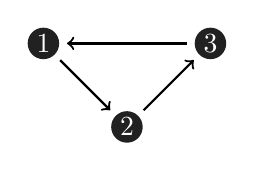
\begin{tikzpicture}[node distance=15mm,
				dot/.style={minimum size=4mm, circle, draw=none, fill=black!87, inner sep=0, outer sep=1mm, text=white}]
				
				\begin{scope}
				\node [dot] (1) {1};
				\node [dot,below right of=1] (2) {2};
				\node [dot,above right of=2] (3) {3};
				\begin{scope}[->,thick]
				\draw (1) -- (2);
				\draw (2) -- (3);
				\draw (3) -- (1);
				\end{scope}
				\end{scope}
				\end{tikzpicture}
			\column{.5\textwidth}
				\[\exists y\forall x Rxy\nvDash\forall y\exists x Rxy\]
				\centering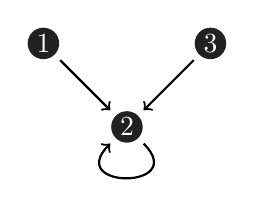
\begin{tikzpicture}[node distance=15mm,
				dot/.style={minimum size=4mm, circle, draw=none, fill=black!87, inner sep=0, outer sep=1mm, text=white}]
				
				\begin{scope}[xshift=50mm]
				\node [dot] (1) {1};
				\node [dot,below right of=1] (2) {2};
				\node [dot,above right of=2] (3) {3};
				\begin{scope}[->,thick]
				\draw (1) -- (2);
				\draw (3) -- (2);
				\draw (2) to[out=-45,in=-45-90,looseness=5] (2);
				\end{scope}
				\end{scope}
				\end{tikzpicture}
		\end{columns}
	\end{block}
\end{frame}

\begin{frame}\frametitle{Is there a finite counter model?}
	\begin{exercise}[Counter Model]
		Give a counter model for
	\begin{enumerate}
		\item $\forall x\exists y Rxy\wedge\forall xyz(Rxy\wedge Ryz\to Rxz)\nvDash\exists x Rxx$
		\item $\forall x\exists y Rxy\wedge\forall xyz(Rxy\wedge Ryz\to Rxz)\nvDash\exists xy(Rxy\wedge Ryx)$
	\end{enumerate}
	\end{exercise}
\begin{prooftree}
	\AxiomC{Everybody loves somebody}
	\noLine
	\UnaryInfC{Everybody loves all persons who are loved by his loved ones}
	\alwaysSingleLine
	\UnaryInfC{There is at least a pair of persons who love each other}
\end{prooftree}
\[(\mathbb{Z},<)\]
\end{frame}

\begin{frame}\frametitle{Mistakes to Avoid}
\[\forall x(Bx\to Sx)\]
\[\exists x(Bx\wedge Sx)\]
\begin{itemize}
	\item $\forall x(Bx\wedge Sx)$\\
	Everyone is a boy and everyone is smart.
	\item $\exists x(Bx\to Sx)$\\
	It is true if there is anyone who is not a boy.
\end{itemize}
\end{frame}

\begin{frame}\frametitle{Coincidence Lemma}
	\begin{lemma}[Coincidence Lemma]
		Assume $\nu_1,\nu_2: \mathcal{V}\to M$, and for all $x\in \operatorname{Fv}(A): \nu_1(x)=\nu_2(x)$. Then
		\[\mathcal{M},\nu_1\vDash A\iff\mathcal{M},\nu_2\vDash A\]
	\end{lemma}
	\begin{itemize}
		\item If $A$ is a sentence, then either $\mathcal{M}\vDash A$ or $\mathcal{M}\vDash\neg A$.
		\item $\mathcal{M}\vDash A\implies\mathcal{M}\vDash\forall x A$
		\item \textbf{Notation}: If $\operatorname{Fv}(A)\subset\{x_1,\dots,x_n\}$, then we write $\mathcal{M}\vDash A[a_1,\dots,a_n]$ to mean $\mathcal{M},\nu\vDash A$ for some \textcolor{yellow}{(equivalently any)} assignment $\nu$ s.t. $\nu(x_i)=a_i$ for $1\leq i\leq n$.
	\end{itemize}
\end{frame}

\begin{frame}\frametitle{Substitution Lemma}
	\begin{columns}
		\column{.57\textwidth}
		\setlength\abovedisplayskip{0pt}
		\setlength\belowdisplayskip{0pt}
			\begin{lemma}[Substitution Lemma]
				\begin{itemize}
					\item $\nu\left(s[t/x]\right)=\nu(\nu(t)/x)(s)$
					\item If the term $t$ is substitutable for the variable $x$ in the wff $A$, then
					\[\mathcal{M},\nu\vDash A[t/x]\iff\mathcal{M},\nu(\nu(t)/x)\vDash A\]
				\end{itemize}
			\end{lemma}
		\column{.38\textwidth}
			\begin{block}{}\hspace*{2em}
						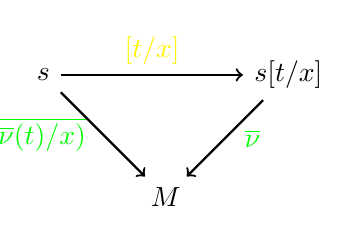
\begin{tikzpicture}[node distance=2.2cm]
						\begin{scope}[->,ultra thick]
						\node (1) {$s$};
						\node [below right of=1] (2) {$M$};
						\node [above right of=2] (3) {$s[t/x]$};
						\begin{scope}[->,ultra thick]
						\draw[thick,->,above] (1) to node{\textcolor{yellow}{$[t/x]$}} (3);
						\draw[thick,->,below of=1] (1) to node{\textcolor{green}{\!\!\!\!\!\!\!\!\!\!\!\!\!\!\!\!\!\!\!\!\!\!\!\!\!\!\!\!\!\!\!\!$\overline{\nu(\overline{\nu}(t)/x)}$}} (2);
						\draw[thick,->,below of=3] (3) to node{\textcolor{green}{\qquad$\overline{\nu}$}} (2);
						\end{scope}
						\end{scope}
						\end{tikzpicture}
			\end{block}
	\end{columns}
	\begin{block}{}
		\[\mathscr{L}_M\coloneqq \mathscr{L}\cup\mathcal{C}_M\;\;\mbox{where}\;\;\mathcal{C}_M\coloneqq \left\{c_a: a\in M\right\}\]
		\[\mathcal{M},\nu\vDash A[c_a/x]\iff\mathcal{M},\nu(a/x)\vDash A\]
		We abbreviate $\mathcal{M},\nu\vDash A[c_a/x]$ by $\mathcal{M},\nu\vDash A[a]$.
		\[\textcolor{yellow}{\mathcal{M},\nu\vDash\forall x A\iff\;\mbox{for every}\; a\in M: \mathcal{M},\nu\vDash A[a]}\]
	\end{block}
\end{frame}

\begin{frame}\frametitle{Equivalent Replacement}
	\begin{lemma}
		Suppose $B\in \operatorname{Sub}(A)$, and $A^*$ arises from $A$ by replacing zero or more occurrences of $B$ by $C$. Then
		\[\vDash B\leftrightarrow C\implies\vDash A\leftrightarrow A^*\]
	\end{lemma}
\end{frame}

\begin{frame}\frametitle{Alphabetic Variant}
	\begin{definition}[Alphabetic Variant]
		If $y\notin \operatorname{Fv}(A)$, and $y$ is substitutable for $x$ in $A$, we say that $\forall y A[y/x]$ is an alphabetic variant of $\forall x A$.
	\end{definition}
	\begin{theorem}
		If $\forall y A[y/x]$ is an alphabetic variant of $\forall x A$, then \[\vDash\forall x A\leftrightarrow\forall y A[y/x]\]
	\end{theorem}
	If $y\notin \operatorname{Fv}(A)$, then $A[y/x][x/y]=A$.
	\begin{itemize}
		\item \textbf{Convention}: When we write $A[t/x]$ we assume that $t$ is substitutable for $x$ in $A$. --- \textit{For any formula $A$ and a finite number of variables $y_1,\dots,y_n$ (occurring in $t$), we can always find a logically equivalent alphabetic variant $A^*$ of $A$ s.t. $y_1,\dots,y_n$ do not occur bound in $A^*$.}
	\end{itemize}
\end{frame}

\begin{frame}\frametitle{Equality and Equivalence}
	\begin{lemma}
		Suppose $\operatorname{Fv}(t)\cup \operatorname{Fv}(s)\subset\{x_1,\dots,x_n\}$, and $A^*$ arises from the wff $A$ by replacing one occurrence of $t$ in $A$ by $s$. Then
		\[\vDash\forall x_1\dots x_n(t=s)\to(A\leftrightarrow A^*)\]
		\[\mathcal{M}\vDash t=s\implies\mathcal{M}\vDash A\leftrightarrow A^*\]
	\end{lemma}
	\begin{lemma}
		Suppose $\operatorname{Fv}(B)\cup \operatorname{Fv}(C)\subset\{x_1,\dots,x_n\}$, and $A^*$ arises from the wff $A$ by replacing one occurrence of $B$ in $A$ by $C$. Then
		\[\vDash\forall x_1\dots x_n(B\leftrightarrow C)\to(A\leftrightarrow A^*)\]
		\[\mathcal{M}\vDash B\leftrightarrow C\implies\mathcal{M}\vDash A\leftrightarrow A^*\]
	\end{lemma}
\end{frame}

\begin{frame}\frametitle{Remark}
	\begin{itemize}
		\item $\vDash\forall x\bigl(Px\leftrightarrow Qx\bigr)\to\bigl(\forall x Px\leftrightarrow\forall x Qx\bigr)$
		
		$\nvDash\bigl(Px\leftrightarrow Qx\bigr)\to\bigl(\forall x Px\leftrightarrow\forall x Qx\bigr)$
		\item $\mathcal{M},\nu\vDash t=s\centernot\implies\mathcal{M},\nu\vDash A\leftrightarrow A^*$
		\item $\mathcal{M},\nu\vDash B\leftrightarrow C\centernot\implies\mathcal{M},\nu\vDash A\leftrightarrow A^*$
		\[B=Px,\;\; C=Py,\;\; A=\forall x Px,\;\; A^*=\forall x Py\]
	\end{itemize}
\end{frame}

\begin{frame}\frametitle{Valid Formulas --- Example}
	\begin{align*}
	&\forall x A\to A[t/x] && A[t/x]\to\exists x A\\
	&\neg\forall x A\leftrightarrow\exists x\neg A &&\neg\exists x A\leftrightarrow\forall x\neg A\\
	&\textcolor{yellow}{\forall x(A\wedge B)\leftrightarrow\forall x A\wedge\forall x B} &&\textcolor{yellow}{\forall x A\vee\forall x B\to\forall x(A\vee B)}\\
	&\textcolor{yellow}{\exists x(A\vee B)\leftrightarrow\exists x A\vee\exists x B} &&\textcolor{yellow}{\exists x(A\wedge B)\to\exists x A\wedge\exists x B}\\
	&\forall x(A\to B)\to\forall x A\to\forall x B &&\forall x(A\to B)\to\exists x A\to\exists x B\\
	&\forall xy A\leftrightarrow\forall yx A &&\exists xy A\leftrightarrow\exists yx A\\
	&\exists x\forall y A\to\forall y\exists x A &&\\
	&\forall x(A\leftrightarrow B)\to(\forall x A\leftrightarrow\forall x B) &&\\
	&(\forall x A\to\exists x B)\leftrightarrow\exists x(A\to B)&&
	\end{align*}
\end{frame}

\begin{frame}\frametitle{Valid Formulas --- Example}
	$x\notin \operatorname{Fv}(A):$
	\hrule
	\begin{align*}
	& A\leftrightarrow\forall x A && A\leftrightarrow\exists x A\\
	&\forall x(A\vee B)\leftrightarrow A\vee\forall x B &&\exists x(A\vee B)\leftrightarrow A\vee\exists x B\\
	&\forall x(A\wedge B)\leftrightarrow A\wedge\forall x B &&\exists x(A\wedge B)\leftrightarrow A\wedge\exists x B\\
	&\forall x(A\to B)\leftrightarrow(A\to\forall x B) &&\exists x(A\to B)\leftrightarrow(A\to\exists x B)\\
	&\textcolor{yellow}{\forall x(B\to A)\leftrightarrow(\exists x B\to A)} &&\textcolor{yellow}{\exists x(B\to A)\leftrightarrow(\forall x B\to A)}\\
	&&&\exists x(A\to\forall x A)
	\end{align*}
\end{frame}

\begin{frame}\frametitle{Valid Formulas --- Example}
	\begin{align*}
	&t=t\\
	&t=s\to s=t\\
	&t=s\to s=r\to t=r\\
	&t_1=s_1\to\dots\to t_n=s_n\to f(t_1,\dots,t_n)=f(s_1,\dots,t_n)\\
	&t_1=s_1\to\dots\to t_n=s_n\to \bigl(P(t_1,\dots,t_n)\leftrightarrow P(s_1,\dots,s_n)\bigr)\\
	&t=s\to r[t/x]=r[s/x]\\
	&t=s\to\bigl(A[t/x]\leftrightarrow A[s/x]\bigr)
	\end{align*}
\end{frame}

\begin{frame}\frametitle{Valid Formulas --- Example}
	$x\notin \operatorname{Fv}(t):$
	\hrule
	\begin{align*}
	&\exists x(x=t)\\
	& A[t/x]\leftrightarrow\exists x (x=t\wedge A)\\
	& A[t/x]\leftrightarrow\forall x(x=t\to A)
	\end{align*}
\end{frame}

\begin{frame}\frametitle{Application --- Game Theory}
	\begin{theorem}[Zermelo's Theorem]
		Every finite game of perfect information with no tie is determined.
	\end{theorem}
	\begin{proof}
		First, color those end nodes black that are wins for player $1$, and color the other end nodes white, being the wins for $2$. Then
		\begin{itemize}
			\item if player $1$ is to move, and at least one child is black, color it black; if all children are white, color it white.
			\item if player $2$ is to move, and at least one child is white, color it white; if all children are black, color it black.
		\end{itemize}
	\end{proof}
	\begin{proof}
		\[\exists x_1\forall y_1\dots\exists x_n\forall y_n A\vee\forall x_1\exists y_1\dots\forall x_n\exists y_n\neg A\]
		where $A$ states that a final position is reached where player $1$ wins.
	\end{proof}
\end{frame}

%%%%%%%%%%%%%%%%%%%%%%%%%%%%%%%
\subsection{Formal Systems}
%%%%%%%%%%%%%%%%%%%%%%%%%%%%%%%

\begin{frame}\frametitle{Formal Systems}
	\begin{itemize}
		\item Hilbert System
		\item Tree Method
		\item Natural Deduction
		\item Sequent Calculus
		\item Resolution
		\item \dots
	\end{itemize}
\end{frame}

%-------------------------------------%
\subsubsection{Hilbert System}
%-------------------------------------%

\begin{frame}\frametitle{Hilbert System $=$ Axiom $+$ Inference Rule}\vspace{-1ex}
				\begin{block}{Axiom Schema}
					\begin{enumerate}
						\item $A\to B\to A$
						\item $(A\to B\to C)\to(A\to B)\to A\to C$
						\item $(\neg A\to\neg B)\to(\neg A\to B)\to A$
						\item \textcolor{yellow}{$\forall x(A\to B)\to\forall x A\to\forall x B$}
						\item \textcolor{yellow}{$\forall x A\to A[t/x]$ where $t$ is substitutable for $x$ in $A$.}
						\item \textcolor{yellow}{$A\to\forall x A$ where $x\notin \operatorname{Fv}(A)$.}
						\item $x=x$
						\item $x=y\to A\to A'$ where $A$ is atomic and $A'$ is obtained from $A$ by replacing $x$ in zero or more places by $y$.
						\item \textcolor{green}{$\forall x_1\dots x_n A$ where $n\geq 0$ and $A$ is any axiom of the preceding groups.}
					\end{enumerate}
				\end{block}
				\begin{block}{Inference Rule}
					\begin{prooftree}
						\AxiomC{$A$\quad$A\to B$}
						\alwaysSingleLine
						\RightLabel{\textcolor{yellow}{[MP]}}
						\UnaryInfC{$B$}
					\end{prooftree}
				\end{block}
\end{frame}

\begin{frame}\frametitle{Example}
	\begin{theorem}
		\[A\vdash\exists x A\]
	\end{theorem}
	\begin{proof}
		\begin{enumerate}
			\item $(\forall x\, \neg A \to \neg A) \to A \to \neg \forall x\, \neg A$ \hfill Tautology
			\item $\forall x\, \neg A \to \neg A$ \hfill A5
			\item $A\to \neg \forall x\, \neg A$ \hfill 1,2 MP
			\item $A$ \hfill Premise
			\item $\neg \forall x\, \neg A$ \hfill 3,4 MP
			\item $\exists x\, A$ \hfill Definition of $\exists$
		\end{enumerate}
	\end{proof}
\end{frame}

\begin{frame}\frametitle{Deduction Theorem}
\begin{theorem}[Deduction Theorem1]
	\[\Gamma, A\vdash B\implies\Gamma\vdash A\to B\]
\end{theorem}
\begin{block}{Inference Rule}
\begin{prooftree}
	\AxiomC{$A$}
	\alwaysSingleLine
	\RightLabel{\textcolor{yellow}{[G]}}
	\UnaryInfC{$\forall x A$}
\end{prooftree}
\end{block}
What if we remove Axiom$9$ and add the rule of generalization to Hilbert System?
\begin{theorem}[Deduction Theorem2]
If $\Gamma, A\vdash B$, where the rule of generalization is not applied to the free variables of $A$, then $\Gamma\vdash A\to B$.
\end{theorem}
\end{frame}

\begin{frame}\frametitle{Meta-properties}
	\begin{itemize}
		\item $\vDash A[B_1/p_1,\dots, B_n/p_n]$ where $A\in\mathscr{L}^0$, $B_1,\dots, B_n\in\mathscr{L}^1$. \hfill \textcolor{yellow}{tautology}
		\item $\Gamma, A\vdash B\wedge\neg B\implies\Gamma\vdash\neg A$\hfill\textcolor{yellow}{reductio ad absurdum}
		\item $\Gamma,\neg A\vdash B\;\;\&\;\;\Gamma,\neg A\vdash\neg B\implies\Gamma\vdash A$ \hfill \textcolor{yellow}{proof by contradiction}
		\item $\Gamma, A\vdash\neg B\iff\Gamma, B\vdash\neg A$\hfill\textcolor{yellow}{contraposition}
		\item $t=s\vdash r[t/x]=r[s/x]$\hfill\textcolor{yellow}{substitution}
		\item $t=s\vdash A[t/x]\leftrightarrow A[s/x]$\hfill\textcolor{yellow}{substitution}
		\item $\vdash B\leftrightarrow C\implies\vdash A\leftrightarrow A^*$ where $A^*$ arises from $A$ by replacing one or more occurrences of $B$ in $A$ by $C$.\hfill \textcolor{yellow}{equivalent replacement}
		\item $\vdash\forall x A\iff\vdash\forall y A[y/x]$ \hfill \textcolor{yellow}{alphabetic variant}
	\end{itemize}
\end{frame}

\begin{frame}\frametitle{Meta-properties}
	\begin{itemize}
		\item \textcolor{yellow}{$\Gamma\vdash A[t/x]\implies\Gamma\vdash\exists x A$\hfill $\exists R$}
		\item \textcolor{yellow}{$\Gamma, A[t/x]\vdash B\implies\Gamma,\forall x A\vdash B$\hfill $\forall L$}
		\item \textcolor{yellow}{$\Gamma, A\vdash B\;\;\&\;\;x\notin \operatorname{Fv}(\Gamma,B)\implies\Gamma,\exists x A\vdash B$\hfill $\exists L$}
		\item \textcolor{yellow}{$\Gamma\vdash A\;\;\&\;\;x\notin\operatorname{Fv}(\Gamma)\implies\Gamma\vdash\forall x A$\hfill $\forall R$}
		\item $\Gamma, A[y/x]\vdash B\;\;\&\;\;y\notin \operatorname{Fv}(\Gamma,\exists x A, B)\implies\Gamma,\exists x A\vdash B$\hfill \textcolor{yellow}{$\exists L$}
		\item $\Gamma\vdash A[y/x]\;\;\&\;\;y\notin\operatorname{Fv}(\Gamma,\forall x A)\implies\Gamma\vdash\forall x A$\hfill \textcolor{yellow}{$\forall R$}
		\item $\Gamma, A[a/x]\vdash B\;\;\&\;\;a\notin\operatorname{Cst}(\Gamma,\exists x A, B)\implies\Gamma,\exists x A\vdash B$\hfill \textcolor{yellow}{$\exists L$}
		\item $\Gamma\vdash A[a/x]\;\;\&\;\;a\notin\operatorname{Cst}(\Gamma,\forall x A)\implies\Gamma\vdash\forall x A$\hfill \textcolor{yellow}{$\forall R$}
		\item $\Gamma\vdash A\;\;\&\;\;a\notin\operatorname{Cst}(\Gamma)\;\;\&\;\; x\notin\operatorname{Fv}(A)\implies\Gamma\vdash\forall x A[x/a]$
	\end{itemize}
\end{frame}

\begin{frame}\frametitle{Alphabetic Variant}
	\begin{theorem}[Existence of Alphabetic Variants]
		Let $A$ be a formula, $t$ a term, and $x$ a variable. Then we can find a formula $A^*$ which differs from $A$ only in the choice of quantified variables s.t.
		\begin{enumerate}
			\item $A\dedeq A^*$
			\item $t$ is substitutable for $x$ in $A^*$.
		\end{enumerate}
	\end{theorem}
\end{frame}

\begin{frame}\frametitle{Strategy}
	\begin{description}
		\item[$\to$] 
		\begin{itemize}
			\item $\Gamma\vdash A\to B\impliedby\Gamma, A\vdash B$
		\end{itemize}
		\item[$\forall$]
		\begin{enumerate}
			\item if $x\notin \operatorname{Fv}(\Gamma)$, $\Gamma\vdash\forall x A\impliedby\Gamma\vdash A$
			\item if $x\in \operatorname{Fv}(\Gamma)$, $\Gamma\vdash\forall x A\impliedby\Gamma\vdash\forall y A[y/x]\impliedby\Gamma\vdash A[y/x]$ for some new $y$.
		\end{enumerate}
		\item[$\neg$]
		\begin{enumerate}
			\item $(\neg\to)$\quad
			$\Gamma\vdash\neg(A\to B)\impliedby\Gamma\vdash A\;\;\&\;\;\Gamma\vdash\neg B$
			\item $(\neg\neg)$\quad $\Gamma\vdash\neg\neg A\impliedby\Gamma\vdash A$
			\item $(\neg\forall)$\quad
			$\Gamma\vdash\neg\forall x A\impliedby\Gamma\vdash\neg A[t/x]$\\ Unfortunately this is not always possible. Try contraposition, reductio ad absurdum or prove by contradiction\dots
		\end{enumerate}
	\end{description}
\end{frame}

%----------------------------------%
\subsubsection{Tree Method}
%----------------------------------%

\begin{frame}\frametitle{Tree Method for Propositional Logic}\vspace{-2ex}
		\begin{columns}
			\column{0.2\textwidth}
				\begin{center}
					\begin{tikzpicture}[sibling distance=10em,
					every node/.style={align=center}]
					\node{$\neg\neg A$}
					child{node{$A$}};
					\end{tikzpicture}
				\end{center}
			\column{0.5\textwidth}
				\begin{center}
					\begin{tikzpicture}[sibling distance=10em,
					every node/.style={align=center}]
					\node{$A\to B$}
					child{node{$\neg A$}}
					child{node{$B$}};
					\end{tikzpicture}
				\end{center}
			\column{0.2\textwidth}
				\begin{center}
					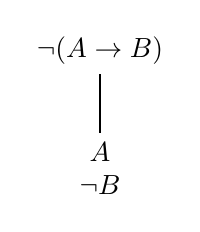
\begin{tikzpicture}[sibling distance=10em,
					every node/.style={align=center}]
					\node{$\neg(A\to B)$}
					child{node{$A$\\$\neg B$}};
					\end{tikzpicture}
				\end{center}
		\end{columns}
		\vspace{7pt}
		\hrule
		\vspace{7pt}
		\begin{columns}
			\column{0.1\textwidth}
				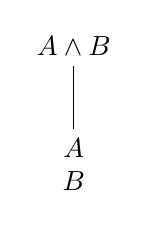
\begin{tikzpicture}[sibling distance=10em,
				every node/.style={align=center}]
				\node{$A\wedge B$}
				child{node{$A$\\$B$}};
				\end{tikzpicture}
			\column{0.35\textwidth}
				\resizebox{\textwidth}{!}{
					\begin{tikzpicture}[sibling distance=10em,
					every node/.style={align=center}]
					\node{$\!\!\!\!\neg(A\wedge B)$}
					child{node{$\neg A$}}
					child{node{$\neg B$}};
					\end{tikzpicture}}
			\column{0.35\textwidth}
				\resizebox{\textwidth}{!}{
					\begin{tikzpicture}[sibling distance=10em,
					every node/.style={align=center}]
					\node{$A\vee B$}
					child{node{$A$}}
					child{node{$B$}};
					\end{tikzpicture}}
			\column{0.12\textwidth}
				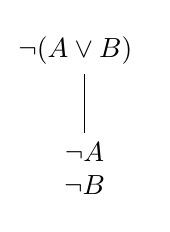
\begin{tikzpicture}[sibling distance=10em,
				every node/.style={align=center}]
				\node{$\!\!\!\!\neg(A\vee B)$}
				child{node{$\neg A$\\$\neg B$}};
				\end{tikzpicture}
		\end{columns}
		\vspace{7pt}
		\hrule
		\vspace{7pt}
		\begin{columns}
			\column{0.35\textwidth}\hspace{-7pt}
				\resizebox{\textwidth}{!}{
					\begin{tikzpicture}[sibling distance=10em,
					every node/.style={align=center}]
					\node{$A\leftrightarrow B$}
					child{node{$A$\\$B$}}
					child{node{$\neg A$\\$\neg B$}};
					\end{tikzpicture}}
			\column{0.35\textwidth}\hspace{-7pt}
				\resizebox{\textwidth}{!}{
					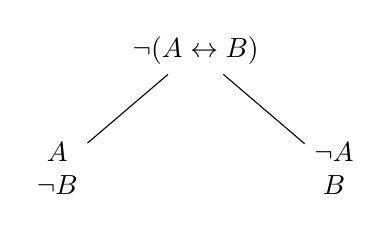
\begin{tikzpicture}[sibling distance=10em,
					every node/.style={align=center}]
					\node{$\neg(A\leftrightarrow B)$}
					child{node{$A$\\$\neg B$}}
					child{node{$\neg A$\\$B$}};
					\end{tikzpicture}}
		\end{columns}
	\[\textcolor{red}{\checkmark}\]
\end{frame}

\begin{frame}\frametitle{Tree Method for Predicate Logic I}
	\textcolor{green}{Ground Tree:}
	\begin{columns}
		\column{0.5\textwidth}
			\begin{center}
				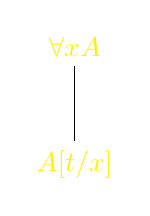
\begin{tikzpicture}[sibling distance=10em,
				every node/.style={align=center}]
				\node{\textcolor{yellow}{$\forall x A$}}
				child{node{\textcolor{yellow}{$A[t/x]$}}};
				\end{tikzpicture}
			\end{center}
			where $t$ is a ground term.
		\column{0.5\textwidth}
			\begin{center}
				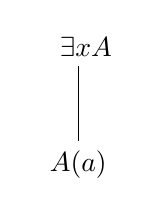
\begin{tikzpicture}[sibling distance=10em,
				every node/.style={align=center}]
				\node{\;\;\;$\exists x A\;\textcolor{red}{\checkmark}$}
				child{node{$A(a)$}};
				\end{tikzpicture}
			\end{center}
			where $a$ is a new constant.
	\end{columns}
	\hrule
	\vspace{7pt}
	\begin{columns}
		\column{0.5\textwidth}
			\begin{center}
				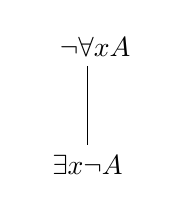
\begin{tikzpicture}[sibling distance=10em,
				every node/.style={align=center}]
				\node{\;\;\;$\neg\forall x A\;\textcolor{red}{\checkmark}$}
				child{node{$\exists x\neg A$}};
				\end{tikzpicture}
			\end{center}
		\column{0.5\textwidth}
			\begin{center}
				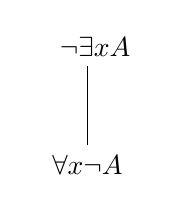
\begin{tikzpicture}[sibling distance=10em,
				every node/.style={align=center}]
				\node{\;\;\;$\neg\exists x A\;\textcolor{red}{\checkmark}$}
				child{node{$\forall x\neg A$}};
				\end{tikzpicture}
			\end{center}
	\end{columns}
\end{frame}

\begin{frame}\frametitle{Tree Method for Predicate Logic II}
	\textcolor{green}{Tree Method with Unification:}
	\begin{columns}
		\column{0.5\textwidth}
			\begin{center}
				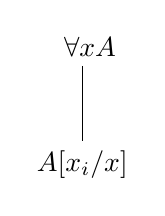
\begin{tikzpicture}[sibling distance=10em,
				every node/.style={align=center}]
				\node{\;\;\;$\forall x A$\;\textcolor{red}{\checkmark}}
				child{node{$A[x_i/x]$}};
				\end{tikzpicture}
			\end{center}
			where $x_i$ is a new variable.
		\column{0.5\textwidth}
			\begin{center}
				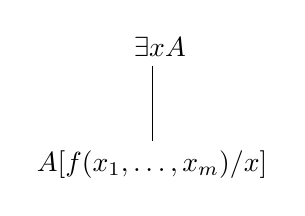
\begin{tikzpicture}[sibling distance=10em,
				every node/.style={align=center}]
				\node{\;\;\;$\exists x A$\;\textcolor{red}{\checkmark}}
				child{node{$A[f(x_1,\dots,x_m)/x]$}};
				\end{tikzpicture}
			\end{center}
			where $f$ is a new function and $\{x_1,\dots,x_m\}=\operatorname{Fv}(\exists x A)$.
	\end{columns}
	\hrule
	\vspace{7pt}
	\begin{columns}
		\column{0.5\textwidth}
			\begin{center}
				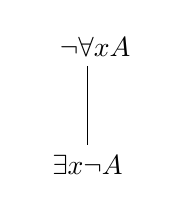
\begin{tikzpicture}[sibling distance=10em,
				every node/.style={align=center}]
				\node{\;\;\;$\neg\forall x A\;\textcolor{red}{\checkmark}$}
				child{node{$\exists x\neg A$}};
				\end{tikzpicture}
			\end{center}
		\column{0.5\textwidth}
			\begin{center}
				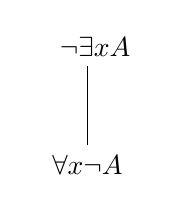
\begin{tikzpicture}[sibling distance=10em,
				every node/.style={align=center}]
				\node{\;\;\;$\neg\exists x A\;\textcolor{red}{\checkmark}$}
				child{node{$\forall x\neg A$}};
				\end{tikzpicture}
			\end{center}
	\end{columns}
\end{frame}

\begin{frame}\frametitle{Tree Method with Unification}
	\begin{itemize}
		\item when expanding a universally quantified formula, do not choose a specific term but a rigid variable as a placeholder.
		\item choose the term only when it is clear it allows closing a branch.
	\end{itemize}
	\begin{center}
		\textcolor{yellow}{rigid variable=same value in the whole tree}
	\end{center}
	\begin{itemize}
		\item variables can assigned to closed terms, like $x_1=a$.
		\item can also be assigned to unclosed terms, like $x_1=f(x_2)$.
	\end{itemize}
	\begin{itemize}
		\item make literals one the opposite of the other.
		\item using terms as unspecified as possible --- Given literals $A$ and $\neg B$ on the same branch, take the \textcolor{yellow}{most general unifier} of $A$ and $B$.
	\end{itemize}
\end{frame}

\begin{frame}\frametitle{Unifier}
\begin{block}{}
\begin{itemize}
\item A substitution $\sigma$ is a \emph{unifier} for a set $\Gamma$ of formulae if for every $A, B\in\Gamma: A\sigma=B\sigma$.
\item A unifier $\sigma$ is a \emph{most general unifier} for $\Gamma$ if for each unifier $\theta$ there exists a substitution $\uplambda$ s.t. $\theta=\sigma\uplambda$.
\end{itemize}
\end{block}
\[\sigma\coloneqq \{t_1/x_1,\dots,t_m/x_m\}\qquad \uplambda\coloneqq \{s_1/y_1,\dots,s_n/y_n\}\]
\[\sigma\uplambda=\big\{t_1\uplambda/x_1,\dots,t_m\uplambda/x_m,\; s_1/y_1,\dots,s_n/y_n\big\}\setminus\big\{s_i/y_i: y_i\in\{x_1,\dots,x_m\}\big\}\]
\begin{itemize}
	\item $(A\sigma)\uplambda=A(\sigma\uplambda)$ and $(t\sigma)\uplambda=t(\sigma\uplambda)$
	\item $(\sigma\uplambda)\theta=\sigma(\uplambda\theta)$
\end{itemize}
\end{frame}

\begin{frame}\frametitle{Tree Method for Predicate Logic}
		\begin{columns}
			\column{0.5\textwidth}
				\begin{center}
					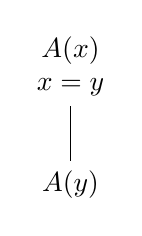
\begin{tikzpicture}[sibling distance=10em,
					every node/.style={align=center}]
					\node{$A(x)$\\$x=y$}
					child{node{$A(y)$}};
					\end{tikzpicture}
				\end{center}
			\column{0.5\textwidth}
				\begin{center}
					\begin{tikzpicture}[sibling distance=10em,
					every node/.style={align=center}]
					\node{$A(x)$\\$y=x$}
					child{node{$A(y)$}};
					\end{tikzpicture}
				\end{center}
		\end{columns}
		\vspace{5pt}
		where $A(y)$ arises from the wff $A(x)$ by replacing one or more occurrences of $x$ by $y$.
\end{frame}

\begin{frame}\frametitle{Deduction \& Tactics}
	\setlength\abovedisplayskip{0pt}
	\setlength\belowdisplayskip{0pt}
	\begin{definition}[Deduction]
		\[A_1,\dots, A_n\vdash B\;\text{iff there exists a closed tree from}\;\{A_1,\dots, A_n,\neg B\}.\]
	\end{definition}
\begin{itemize}
	\item Try to apply ``non-branching'' rules first, in order to reduce the number of branches.
	\item Try to close off branches as quickly as possible.
	\item Deal with negated quantifiers first.
	\item Instantiate existentials before universals.
\end{itemize}
\end{frame}

\begin{frame}\frametitle{Example --- Ground Tree}
	\centering\fbox{$\big\{\forall x\neg P(x),\exists x(P(x)\vee P(f(x)))\big\}$ is unsatisfiable.}
	\begin{center}
		\begin{tikzpicture}[sibling distance=10em, every node/.style={align=center}]
		\node{$\forall x\neg P(x)$\\$\quad\exists x(P(x)\vee P(f(x)))\;\checkmark$}
		child{node{$\quad P(a)\vee P(f(a))\;\checkmark$}
			child{node{$P(a)$}
				child{node{$\neg P(a)$\\$\times$}}}
			child{node{$P(f(a))$}
				child{node{$\neg P(f(a))$\\$\times$}}}};
		\end{tikzpicture}
	\end{center}
\end{frame}

\begin{frame}\frametitle{Example --- Tree Method with Unification}
	\centering\fbox{$\big\{\forall xP(x),\neg Q(f(a)),\forall x(\neg P(f(x))\vee Q(x))\big\}$ is unsatisfiable.}
	\begin{center}
		\begin{tikzpicture}[sibling distance=10em,
		every node/.style={align=center}]
		\node{$\quad\forall x P(x)\;\checkmark$\\$\neg Q(f(a))$\\$\quad\forall x(\neg P(f(x))\vee Q(x))\;\checkmark$}
		child{node{$P(x_1)$}
			child{node{$\quad\neg P(f(x_2))\vee Q(x_2)\;\checkmark$}
				child{node{$\neg P(f(x_2))$\\ {\footnotesize$x_1=f(x_2)$}\\$\times$}}
				child{node{$Q(x_2)$\\ {\footnotesize $x_2=f(a)$}\\$\times$}}}};
		\end{tikzpicture}
	\end{center}
\end{frame}

\begin{frame}\frametitle{Unification --- Greedy Unification (incomplete)}\vspace{-2ex}
	\begin{center}
		\begin{tikzpicture}[sibling distance=10em,
		every node/.style={align=center}]
		\node{$\quad\neg P(a)\;\checkmark$\\$\quad\neg Q(c)\;\checkmark$\\$\quad\neg R(d)\;\checkmark$\\$\forall x(((R(d)\vee\neg P(b))\wedge P(x))\vee((R(d)\vee\neg Q(b))\wedge Q(x)))\;\checkmark$}
		child{node{\;$\quad((R(d)\vee\neg P(b))\wedge P(x_1))\vee((R(d)\vee\neg Q(b))\wedge Q(x_1))\;\checkmark$}
			child{node{$\!\!\!\!\!\!\!\!\!\!\!\!\!\!\!\!\!\!\!\!\!\!\!\quad(R(d)\vee\neg P(b))\wedge P(x_1)\;\checkmark$}
				child{node{$\;\;R(d)\vee\neg P(b)$\\
				$P(x_1)$\\
				{\footnotesize$x_1=a$}\\$\times$}}}
			child{node{$\qquad(R(d)\vee\neg Q(b))\wedge Q(a)\;\checkmark$}
				child{node{$\quad\;\;\; R(d)\vee\neg Q(b)\;\checkmark$\\
				$Q(a)$}
					child{node{$R(d)$\\$\times$}}
					child{node{$\neg Q(b)$}}}}};
		\end{tikzpicture}
	\end{center}\vspace{-2ex}
{\small Applying unification as soon as a branch can be closed by lead to incompleteness.}
\end{frame}

\begin{frame}\frametitle{Unification --- Final Closure}\vspace{-2ex}
	\begin{center}
		\begin{tikzpicture}[sibling distance=10em,
		level distance=3.8em,
		every node/.style={align=center}]
		\node{$\quad\neg P(a)\;\checkmark$\\$\quad\neg Q(c)\;\checkmark$\\$\quad\neg R(d)\;\checkmark$\\$\forall x(((R(d)\vee\neg P(b))\wedge P(x))\vee((R(d)\vee\neg Q(b))\wedge Q(x)))\;\checkmark$}
		child{node{\;$\quad((R(d)\vee\neg P(b))\wedge P(x_1))\vee((R(d)\vee\neg Q(b))\wedge Q(x_1))\;\checkmark$}
			child{node{$\!\!\!\!\!\!\!\!\!\!\!\!\!\!\!\!\!\!\!\!\!\!\!\quad(R(d)\vee\neg P(b))\wedge P(x_1)\;\checkmark$}
				child{node{$\quad\;\;R(d)\vee\neg P(b)\;\checkmark$\\
				$P(x_1)$}
					child{node{$R(d)$\\$\times$}}
					child{node{{}\\{}\\{}\\$\!\!\!\!\!\!\!\!\!\!\!\!\!\!\!\neg P(b)$\\
					{\footnotesize$\!\!\!\!\!\!\!\!\!\!\!\!\!\!\!x_1=b$}\\$\!\!\!\!\!\!\!\!\!\!\times$}}}}
			child{node{$\qquad(R(d)\vee\neg Q(b))\wedge Q(x_1)\;\checkmark$}
				child{node{$\quad\;\;\,R(d)\vee\neg Q(b)\;\checkmark$\\
				$Q(x_1)$}
					child{node{$\qquad\qquad R(d)$\\$\qquad\qquad \times$}}
					child{node{$\neg Q(b)$\\
				{\footnotesize$x_1=b$}\\$\times$}}}}};
		\end{tikzpicture}
	\end{center}\vspace{-2ex}
{\small Unification is applied only when it closes all open branches at the same time.}
\end{frame}

\begin{frame}\frametitle{Example --- Unification vs Ground}
			\centering\fbox{There is someone such that if he is drinking, then everyone is drinking.}
	\begin{columns}
		\column{0.5\textwidth}
			\begin{center}
			\fbox{$\vdash\exists x\big(A(x)\to\forall x A(x)\big)$}
				\begin{tikzpicture}[level distance=3.7em,
				every node/.style={align=center}]
				\node{$\quad\neg\exists x(A(x)\to\forall x A(x))\;\checkmark$}
				child{node{$\quad\forall x\neg(A(x)\to\forall x A(x))\;\checkmark$}
					child{node{$\quad\neg(A(x_1)\to\forall x A(x))\;\checkmark$}
						child{node{$A(x_1)$\\$\quad\neg\forall x A(x)\;\checkmark$}
							child{node{$\neg A(a)$\\{\footnotesize $x_1=a$}\\$\times$}}}}};
				\end{tikzpicture}
			\end{center}
		\column{0.5\textwidth}\vspace{-5pt}
			\begin{center}
				\begin{tikzpicture}[level distance=3.3em,
				every node/.style={align=center}]
				\node{$\forall x\neg(A(x)\to\forall x A(x))$}
				child{node{$\quad\neg(A(a)\to\forall x A(x))\;\checkmark$}
					child{node{$A(a)$\\$\quad\neg\forall x A(x)\;\checkmark$}
						child{node{$\neg A(b)$}
							child{node{$\quad\neg(A(b)\to\forall x A(x))\;\checkmark$}
								child{node{$A(b)$\\$\neg\forall x A(x)$\\$\times$}}}}}};
				\end{tikzpicture}
			\end{center}
	\end{columns}
\end{frame}

\begin{frame}\frametitle{Soundness \& Completeness}
\setlength\abovedisplayskip{0pt}
	\begin{theorem}[Soundness Theorem]
		If the tree closes, the set is unsatisfiable.
	\end{theorem}
	\begin{theorem}[Completeness Theorem]
		If a set is unsatisfiable, there \textcolor{yellow}{exists} a closed tree from it.
	\end{theorem}
	\[A_1,\dots, A_n\vdash B\iff A_1,\dots, A_n\vDash B\]
	\textbf{Remark:} If an inference with predicate wff is not valid and its counterexample is an infinite model, the tree will not find it. The tree method can't generate every counterexample of an invalid inference in predicate logic.
\end{frame}

\begin{frame}\frametitle{Exercises --- Tree Method}
		\begin{enumerate}
			\item $\forall x(Px\to Qx)\to\exists xPx\to\exists xQx$
			\item $\exists x\forall yRxy\to\forall y\exists xRxy$
			\item $\exists x(Px\wedge Qx)\to\exists xPx\wedge\exists xQx$
			\item $\forall x\big(A\vee B(x)\big)\to A\vee\forall x B(x)$ where $x\notin \operatorname{Fv}(A)$
			\item $\exists x\Big(\big(Px\wedge\forall y(Py\to y=x)\big)\wedge Qx\Big)\dedeq\exists x\forall y\Big(\big(Py\leftrightarrow y=x\big)\wedge Qx\Big)$
			\item $\exists x\big(Px\wedge\forall y(Py\to y=x)\big)\wedge\exists x\big(Qx\wedge\forall y(Qy\to y=x)\big)\wedge\neg\exists x(Px\wedge Qx)\to\exists xy\big(x\ne y\wedge (Px\vee Qx)\wedge(Py\vee Qy)\wedge\forall z(Pz\vee Qz\to z=x\vee z=y)\big)$
\[1+1=2\]
		\end{enumerate}
\end{frame}

\begin{frame}\frametitle{Exercises --- Tree Method}%\vspace*{-5pt}
		\begin{enumerate}
			\item Nobody trusts \emph{exactly} those who have no mutual trust with anybody.
			\item If dogs are animals, every head of a dog is the head of an animal.
			\item Every non-analytic, meaningful proposition is either verifiable or falsifiable. Philosophical propositions are neither analytic nor verifiable or falsifiable. Therefore, they are meaningless.
			\item No girl loves any sexist pig. Caroline is a girl who loves whoever loves her. Henry loves Caroline. Thus Henry isn't a sexist pig.
			\item \emph{The} present king of France is bald. Bald men are sexy. Hence whoever is a present King of France is sexy.
			\item \emph{Only} Russell is a great philosopher. Wittgenstein is a great philosopher who smokes. So Russell smokes.
			\item Everyone is afraid of Dracula. Dracula is afraid \emph{only} of me. Therefore, I am Dracula.
			\item Everyone loves a \emph{lover}(\emph{anyone who loves somebody}). Romeo loves Juliet. Therefore, I love you.
			\item Everyone loves a \emph{lover}(\emph{anyone who loves somebody}); hence if someone is a lover, everyone loves everyone!
		\end{enumerate}
\end{frame}

\begin{frame}\frametitle{Exercises --- Tree Method}
		\begin{enumerate}
			\item I am a philosopher. A philosopher can \emph{only} be appreciated by philosophers. No philosopher is without some eccentricity. I sing rock. Every eccentric rock singer is appreciated by some girl. Eccentrics are conceited. Therefore, some girl is conceited.
			\item Any philosopher admires some logician. Some students admire \emph{only} film stars. No film stars are logicians. Therefore not all students are philosophers.
			\item If anyone speaks to anyone, then someone introduces them; no one introduces anyone to anyone unless he knows them both; everyone speaks to Frank; therefore everyone is introduced to Frank by someone who knows him.
			\item Whoever stole the goods, knew the safe combination. Someone stole the goods, and \emph{only} Jack knew the safe combination. Hence Jack stole the goods.
			\item \emph{No one but} Alice and Bette (\emph{who are different people}) admires Carl. All and only those who admire Carl love him. Hence \emph{exactly} two people love Carl.
		\end{enumerate}
\end{frame}

\begin{frame}\frametitle{Application --- \href{http://web.mat.bham.ac.uk/R.W.Kaye/minesw/}{Minesweeper}}\vspace{-5pt}
	\begin{figure}
		\includegraphics[width=0.3\textwidth,angle=0,origin=c]{img/minesweeper}
	\end{figure}\vspace{-7pt}
	\begin{itemize}
		\item There are exactly $n$ mines in the game.
		\item If a cell contains the number $1$, then there is exactly one mine in the adjacent cells.\\
		$\forall x(\operatorname{contain}(x,1)\to\exists y(\operatorname{adj}(x,y)\wedge \operatorname{mine}(y)\wedge\forall z(\operatorname{adj}(x,z)\wedge \operatorname{mine}(z)\to z=y)))$
		\item \dots
	\end{itemize}
\end{frame}

\begin{frame}\frametitle{Russell's Theory of Descriptions}
\begin{columns}
\column{.6\textwidth}
\begin{enumerate}
	\item \textcolor{yellow}{The substitution of identicals.}
	\underline{``The morning star is the evening star.''}
	\item \textcolor{yellow}{The law of the excluded middle.}
	\underline{``The present King of France is bald.''}\;\;\textcolor{red}{or}
	\underline{``The present King of France is not bald.''}
	\item \textcolor{yellow}{The problem of negative existentials.}
	\underline{``The round square is round.''}
\end{enumerate}
\column{.25\textwidth}
\begin{figure}
\includegraphics[width=\textwidth]{img/triangle-centroid-median}
\end{figure}
\end{columns}
\end{frame}

\begin{frame}\frametitle{Russell's Theory of Descriptions}
\begin{align*}
\textcolor{yellow}{B(\iota_x A):}&\textcolor{yellow}{=\exists! x A\wedge\exists x(A\wedge B)}\\
&\textcolor{yellow}{\semeq\exists x\forall y\Big(\big(A(y)\leftrightarrow y=x\big)\wedge B(x)\Big)}
\end{align*}
\textcolor{red}{The} round square does not exist. \textcolor{green}{$B(\iota_x A)\vee(\neg B)(\iota_x A)$}\;\textcolor{red}{?}
\[\exists x\forall y\Big(\big(Ry\wedge Sy\leftrightarrow y=x\big)\wedge\neg Ex\Big)\quad\textcolor{green}{(\neg B)(\iota_x A)}\;\textcolor{red}{?}\]
\[\neg\exists x\forall y\Big(\big(Ry\wedge Sy\leftrightarrow y=x\big)\wedge Ex\Big)\quad\textcolor{green}{\neg B(\iota_x A)}\;\textcolor{red}{?}\]
\[Ex\stackrel{\textcolor{red}{?}}{\coloneqq }\exists P\big(Px\wedge\exists y\neg Py\big)\]
\[\iota_x A=\iota_x A\;\;\textcolor{red}{?}\qquad \forall x B\to B(\iota_x A)\;\;\textcolor{red}{?}\]
\[\textcolor{yellow}{B(\iota_x^y A)\coloneqq \big(\exists!x A\to\exists x(A\wedge B)\big)\wedge\big(\neg\exists!x A\to B[y/x]\big)}\]
\[\vdash\forall x B\to B(\iota_x^y A)\]
\end{frame}

%----------------------------%
\subsection{Definability \& Isomorphism}
%----------------------------%

\begin{frame}\frametitle{Definability}
\begin{block}{}
	\begin{center}
		\textcolor{red}{What is ``definability''?}
	\end{center}
\end{block}
\begin{block}{Berry Paradox}
	The smallest positive integer not definable in fewer than twelve words.
\end{block}
\begin{definition}[Definability]
\begin{itemize}
	\item $X\subset M^n$ is $Y$-definable \emph{($X\in\operatorname{Def}(\mathcal{M},Y)$)} over $\mathcal{M}$ if there is a wff $A$ and $b_1,\dots,b_m\in Y^m$ s.t.
	\[X=\big\{(a_1,\dots,a_n): \mathcal{M}\vDash A[a_1,\dots,a_n,b_1,\dots,b_m]\big\}\]
	\item $X$ is definable in $\mathcal{M}$ if it is $\emptyset$-definable in $\mathcal{M}$.
\end{itemize}
\end{definition}
\begin{quote}
	A definition is acceptable only on condition that it implies no contradiction.\par\hfill --- \textsl{Poincar\'e}
\end{quote}
\end{frame}

\begin{frame}\frametitle{Representability}
	\begin{block}{}
		\begin{center}
			\textcolor{red}{What is ``representability''?}
		\end{center}
	\end{block}
	\begin{definition}[Representable Functions]
		A $n$-ary function $f:\mathbb{N}^n\to\mathbb{N}$ is representable in the theory $\mathrm{T}$ iff there is a wff $A(x_1,\dots,x_n,y)$ s.t. for all $a_1,\dots,a_n$,
	\setlength\belowdisplayskip{0pt}
		\[\mathrm{T}\vdash\forall y\Big(A(\underline{a_1},\dots,\underline{a_n},y)\leftrightarrow y=\underline{f(a_1,\dots,a_n)}\Big)\]
	\end{definition}
	\begin{definition}[Representable Relations]
		A $n$-ary relation $R\subset\mathbb{N}^n$ is representable in the theory $\mathrm{T}$ iff there is a wff $A$ s.t. for all $a_1,\dots,a_n$,
	\setlength\abovedisplayskip{0pt}
	\setlength\belowdisplayskip{0pt}
		\begin{align*}
		&(a_1,\dots,a_n)\in R\implies \mathrm{T}\vdash A[a_1,\dots,a_n]\\
		&(a_1,\dots,a_n)\notin R\implies \mathrm{T}\vdash\neg A[a_1,\dots,a_n]
		\end{align*}
	\end{definition}
	\centering\fbox{A function/relation is representable in Robinson $\mathrm{Q}$ iff it is computable.}
\end{frame}

\begin{frame}\frametitle{Example}
	\begin{itemize}
		\item The interval $[0,\infty)$ is definable in $\mathcal{R}=(\mathbb{R},0,1,+,\cdot)$, where the language is $\mathscr{L}=\{0,1,+,\cdot\}$.
		\[\mathcal{R}\vDash\exists y(x=y\cdot y)[a]\iff a\geq 0\]
		\item The ordering relation $<$ is definable in $\mathcal{N}=(\mathbb{N},0,S,+,\cdot)$, where the language is $\mathscr{L}=\{0,S,+,\cdot\}$.
		\[\exists z\bigl(x+S(z)=y\bigr)\]
		\item The set of primes is definable in $\mathcal{N}$ by the formula
		\[\exists y\bigl(x=S(0)+S(y)\bigr)\wedge\forall yz\bigl(x=y\cdot z\to y=S(0)\vee z=S(0)\bigr)\]
		\item $\mathbb{N}$ is definable in $(\mathbb{Z},+,\cdot)$ by
		\[\exists y_1y_2y_3y_4\Big(x=y_1^2+y_2^2+y_3^2+y_4^2\Big)\tag{\text{Lagrange four-square theorem}}\]
		\item Exponentiation $\big\{(m,n,p): p=m^n\big\}$ is definable in $\mathcal{N}$. (use the Chinese remainder theorem)
	\end{itemize}
\end{frame}

\begin{frame}\frametitle{Homomorphism \& Isomorphism}
\setlength\abovedisplayskip{0pt}
\setlength\belowdisplayskip{0pt}
	\begin{definition}[Homomorphism]
		A homomorphism $h$ of $\mathcal{M}$ into $\mathcal{N}$ is a function $h: M\to N$ s.t.
		\begin{itemize}
			\item For each $n$-place predicate symbol $P$ and each $n$-tuple $(a_1,\dots,a_n)\in M^n$,
			\[(a_1,\dots,a_n)\in P^{\mathcal{M}}\iff(h(a_1),\dots,h(a_n))\in P^{\mathcal{N}}\]
			\item For each $n$-place function symbol $f$ and each $n$-tuple $(a_1,\dots,a_n)\in M^n$,
			\[h: f^{\mathcal{M}}(a_1,\dots,a_n)\mapsto f^{\mathcal{N}}\bigl(h(a_1),\dots,h(a_n)\bigr)\]
			In the case of a constant symbol $c$ this becomes $h: c^{\mathcal{M}}\mapsto c^{\mathcal{N}}$.
		\end{itemize}
	\end{definition}
	\begin{itemize}
		\item An isomorphism \textcolor{yellow}{(monomorphism/epimorphism)} is a bijective \textcolor{yellow}{(injective/surjective)} homomorphism. $\mathcal{M}\cong\mathcal{N}$
		\item An automorphism \textcolor{yellow}{(endomorphism)} is an isomorphism \textcolor{yellow}{(homomorphism)} from $\mathcal{M}$ to itself.
		\item A structure $\mathcal{M}$ is rigid if it has no automorphisms other than $1_M$.
	\end{itemize}
\end{frame}

\begin{frame}\frametitle{Homomorphism Theorem}
	\begin{theorem}[Homomorphism Theorem]
		Let $h$ be a homomorphism of $\mathcal{M}$ into $\mathcal{N}$, and $\nu: \mathcal{V}\to M$.
		\begin{enumerate}
			\item For any term $t$, $h\bigl(\overline{\nu}(t)\bigr)=\overline{h\circ\nu}(t)$
			\item For any \textcolor{yellow}{open} formula $A$ \textcolor{yellow}{not containing $=$}, $\mathcal{M},\nu\vDash A\iff\mathcal{N},h\circ\nu\vDash A$
			\item If $h: M\rightarrowtail N$, we may delete the restriction ``not containing $=$''.
			\item If $h: M\twoheadrightarrow N$, we may delete the restriction ``open''.
		\end{enumerate}
	\end{theorem}
	\begin{definition}[Elementary Equivalence]
		\[\mathcal{M}\equiv\mathcal{N} \text{ if for any sentence}\; A: \mathcal{M}\vDash A\iff\mathcal{N}\vDash A\]
	\end{definition}
	\[\mathcal{M}\cong\mathcal{N}\implies\mathcal{M}\equiv\mathcal{N}\]
\end{frame}

\begin{frame}\frametitle{Substructure}
	\begin{definition}[Substructure]
		$\mathcal{M}$ is called a \emph{substructure} of $\mathcal{N}$ ($\mathcal{M}\subset\mathcal{N}$) iff
		\begin{itemize}
			\item $M\subset N$
			\item
			\begin{enumerate}
				\item $P^{\mathcal{M}}=P^{\mathcal{N}}\cap M^n$ for any $n$-ary predicate symbol $P$.
				\item $f^{\mathcal{M}}=f^{\mathcal{N}}{\restriction_{M^n}}$ for any $n$-ary function symbol $f$.
			\end{enumerate}
		\end{itemize}
	\end{definition}
	\begin{block}{}
	Suppose $\mathcal{M}\subset\mathcal{N}$. Then
		\begin{itemize}
			\item for any term $t(x_1,\dots,x_n)$, and any $a_1,\dots,a_n\in M$,
			\[t^{\mathcal{M}}[a_1,\dots,a_n]=t^{\mathcal{N}}[a_1,\dots,a_n]\]
			\item for any open formula $A(x_1,\dots,x_n)$, and any $a_1,\dots,a_n\in M$,
			\[\mathcal{M}\vDash A[a_1,\dots,a_n]\iff\mathcal{N}\vDash A[a_1,\dots,a_n]\]
		\end{itemize} 
	\end{block}
\end{frame}

\begin{frame}\frametitle{Example}
	\begin{itemize}
		\item 
		$\mathscr{L}=\{0,1,+,\cdot\}, \mathcal{N}=\left(\mathbb{N},0,1,+,\cdot\right), \mathcal{R}=\left(\mathbb{R},0,1,+,\cdot\right)$
		\[\mathcal{N}\subset\mathcal{R}\]
		\item $\mathscr{L}=\{<\}, \mathcal{M}=\left(\mathbb{N},<\right), \mathcal{N}=\left(\left\{2n: n\in\mathbb{N}\right\},<\right)$
		\[h: n\mapsto 2n, \quad h:\mathcal{M}\cong\mathcal{N},\quad\text{but}\quad\mathcal{M}\not\subset\mathcal{N}\]
		\item $\mathscr{L}=\{0,+\}$
		\begin{align*}
		&\mathcal{M}=\big(\mathbb{N},0^{\mathcal{M}},+^{\mathcal{M}}\big), &\text{where}\quad&0^{\mathcal{M}}=0, &&+^{\mathcal{M}}(a,b)=a+b\\
		&\mathcal{N}=\big(\left\{2^n: n\in\mathbb{N}\right\}, 0^{\mathcal{N}}, +^{\mathcal{N}}\big), &\text{where}\quad&0^{\mathcal{N}}=1, &&+^{\mathcal{N}}(a,b)=a\cdot b
		\end{align*}
		\[h: n\mapsto 2^n,\quad h:\mathcal{M}\cong\mathcal{N}\quad\text{but}\quad\mathcal{M}\not\subset\mathcal{N}.\]
	\end{itemize}
\end{frame}

\begin{frame}\frametitle{Example}
	\begin{columns}
		\column{0.3\textwidth}
			\begin{figure}
				\includegraphics[width=\textwidth,angle=0,origin=c]{img/isomorphism-a}
			\end{figure}
		\column{0.5\textwidth}
			\begin{figure}
				\includegraphics[width=\textwidth,angle=0,origin=c]{img/isomorphism-b}
			\end{figure}
			\[\href{http://people.cs.uchicago.edu/~laci/update.html}{quasipolynomial}\;\;2^{O\left((\log n)^c\right)}\]
		\column{0.2\textwidth}
			\begin{align*}
			a&\mapsto 1\\
			b&\mapsto 6\\
			c&\mapsto 8\\
			d&\mapsto 3\\
			g&\mapsto 5\\
			h&\mapsto 2\\
			i&\mapsto 4\\
			j&\mapsto 7
			\end{align*}
	\end{columns}
\end{frame}

\begin{frame}\frametitle{\href{https://mathoverflow.net/questions/53122/mathematical-urban-legends}{A Joke}}
	\begin{figure}
	\includegraphics[width=\textwidth]{img/joke-isomorphic}
	\end{figure}
\end{frame}

\begin{frame}\frametitle{Automorphism \& Undefinability}
	\begin{corollary}
		Let $h$ be an automorphism $h: M\to M$, and $R\subset M^n$ definable in $\mathcal{M}$. Then for any $a_1,\dots,a_n\in M$,
		\[(a_1,\dots,a_n)\in R\iff(h(a_1),\dots,h(a_n))\in R\]
	\end{corollary}
	\textbf{Remark:} This corollary is sometimes useful in showing that a given relation is not definable.
	\begin{block}{The set $\mathbb{N}$ is not definable in $(\mathbb{R},<)$ where $\mathscr{L}=\{<\}$.}
		$h: a\mapsto a^3$ is an automorphism of $\mathbb{R}$.\\
		It maps points outside of $\mathbb{N}$ into $\mathbb{N}$.
	\end{block}
	\begin{center}
		\fbox{$\mathbb{N}$ is not definable in $(\mathbb{R},0,1,+,\cdot,<)$}\\
		Natural numbers are not definable over the theory of real-closed fields.
	\end{center}
\end{frame}

\begin{frame}\frametitle{Example}
	%\setlength\abovedisplayskip{0pt}
\setlength\belowdisplayskip{0pt}
\begin{block}{Example}
	The structure $\mathcal{M}\coloneqq \big(\{a,b,c\},\{(a,b),(a,c)\}\big)$\\
	where the language is $\mathscr{L}=\{E\}$.
	\[b\;\bullet\mathbf{\leftarrow}\stackrel{a}{\bullet}\mathbf{\to}\bullet\;c\]
	\begin{itemize}
		\item $\{b,c\}$ is definable in $\mathcal{M}$:\quad $\exists y E(y,x)$
		\item $\{b\}$ is not definable in $\mathcal{M}$.
	\end{itemize}
\end{block}
\begin{block}{Example}
Consider the vector space $\mathcal{E}\coloneqq (E,+,f_r)_{r\in\mathbb{R}}$, where $E$ is the universe, $f_r$ is the scalar multiplication by $r$.
\begin{itemize}
	\item $U\coloneqq \{\mathbf{x}\in E: |\mathbf{x}|=1\}$ is not definable in $\mathcal{E}$.
	\item $h:\mathbf{x}\mapsto 2\mathbf{x}$ is an automorphism but it does not preserve $U$.
\end{itemize}
\end{block}
\end{frame}

%%%%%%%%%%%%%%%%%%%%%%%%%%%%
\subsection{What is Logic?}
%%%%%%%%%%%%%%%%%%%%%%%%%%%%

\begin{frame}\frametitle{What is Logic?}
	\begin{itemize}
		\item Arithmetic --- the study of numbers.
		\item Geometry --- the study of figures.
		\item Algebra --- the study of mathematical symbols.
		\item Set Theory --- the study of sets.
		\item Logic --- the study of logical notions.
	\end{itemize}
	\begin{itemize}
		\item What is a number?
		\item What is a line?
		\item What is a set?
		\item What is a logical notion?
	\end{itemize}
\end{frame}

\begin{frame}\frametitle{What is Mathematics?}
	\begin{quote}
		Mathematics is the art of giving the same name to different things.\par
		\hfill --- \textsl{Henri Poincar\'e}
		
		Not substance but invariant form is the carrier of the relevant mathematical information.\par
		\hfill --- \textsl{F. William Lawvere}
		
		Mathematics may be defined as the subject in which we never know what we are talking about, nor whether what we are saying is true.\par
		\hfill --- \textsl{Bertrand Russell}
	\end{quote}
\end{frame}

\begin{frame}\frametitle{What is Geometry? --- Klein's Erlangen Program}
	\begin{block}{What is Geometry?}
		The study of \emph{invariants} under \emph{a group of transformations}.
	\end{block}
	\begin{columns}
		\column{0.63\textwidth}
		\boxed{\vbox{\resizebox{0.82\textwidth}{!}{\begin{minipage}{\textwidth}
						\begin{tikzpicture}[scale=0.5]
						\draw[green!50!gray,fill=green!50!gray,nearly transparent,opacity=.5] (0,0) -- (3,0) -- (3,3) -- (0,3) -- cycle;
						\draw[green!50!gray,fill=green!50!gray,nearly transparent,opacity=.5] (5.5,0) -- (8.5,0) -- (8.5,3) -- (5.5,3) -- cycle;
						\node at (14,1.5) {\huge isometry};
						\end{tikzpicture}
						
						\begin{tikzpicture}[scale=0.5]
						\draw[green!50!gray,fill=green!50!gray,nearly transparent,opacity=.5] (0,0) -- (3,0) -- (3,3) -- (0,3) -- cycle;
						\draw[green!50!gray,fill=green!50!gray,nearly transparent,opacity=.5] (5,-.5) -- (9,-.5) -- (9,3.5) -- (5,3.5) -- cycle;
						\node at (14,1.5) {\huge similarity};
						\end{tikzpicture}
						
						\begin{tikzpicture}[scale=.5]
						\draw[green!50!gray,fill=green!50!gray,nearly transparent,opacity=.5] (0,0) -- (3,0) -- (3,3) -- (0,3) -- cycle;
						\draw[green!50!gray,fill=green!50!gray,nearly transparent,opacity=.5] (5,1.5) -- (7,0.5) -- (9,1.5) -- (7,2.5) -- cycle;
						\node at (14,1.5) {\huge affinity};
						\end{tikzpicture}
						
						\begin{tikzpicture}[scale=.5]
						\draw[green!50!gray,fill=green!50!gray,nearly transparent,opacity=.5] (0,0) -- (3,0) -- (3,3) -- (0,3) -- cycle;
						\draw[green!50!gray,fill=green!50!gray,nearly transparent,opacity=.5] (5,0.5) -- (9,0.5) -- (8,2.5) -- (6,2.5) -- cycle;
						\node at (14,1.5) {\huge projection};
						\end{tikzpicture}
						
						\begin{tikzpicture}[scale=.5]
						\coordinate (O) at (0,0,0);
						\coordinate (A) at (0,2,0);
						\coordinate (B) at (0,2,2);
						\coordinate (C) at (0,0,2);
						\coordinate (D) at (2,0,0);
						\coordinate (E) at (2,2,0);
						\coordinate (F) at (2,2,2);
						\coordinate (G) at (2,0,2);
						\draw[green!50!gray,fill=green!50!gray,nearly transparent,opacity=.5] (O) -- (C) -- (G) -- (D) -- cycle;% Bottom Face
						\draw[green!50!gray,fill=green!50!gray!50,nearly transparent,opacity=.5] (O) -- (A) -- (E) -- (D) -- cycle;% Back Face
						\draw[green!50!gray,fill=green!50!gray!50,nearly transparent,opacity=.5] (O) -- (A) -- (B) -- (C) -- cycle;% Left Face
						\draw[green!50!gray,fill=green!50!gray!50,nearly transparent,opacity=.5] (D) -- (E) -- (F) -- (G) -- cycle;% Right Face
						\draw[green!50!gray,fill=green!50!gray!50,nearly transparent,opacity=.5] (C) -- (B) -- (F) -- (G) -- cycle;% Front Face
						\draw[green!50!gray,fill=green!50!gray!50,nearly transparent,opacity=.5] (A) -- (B) -- (F) -- (E) -- cycle;% Top Face
						\end{tikzpicture}\qquad\quad\;
						\begin{tikzpicture}
						\node[circle,shading=ball,fill=green!50!gray,nearly transparent,opacity=.5,minimum width=1.5cm] (ball) at (0,0) {};
						\node at (3.5,0) {\huge continuous};
						\end{tikzpicture}
		\end{minipage}}}}
		\column{0.21\textwidth}\vspace{-4pt}
		\begin{figure}[H]
			\begin{center}
				\includegraphics[width=\textwidth,angle=0,origin=c]{img/klein}\caption{\scriptsize Felix Klein}
			\end{center}
		\end{figure}
	\end{columns}
\end{frame}

\begin{frame}\frametitle{What is Geometry? --- Klein's Erlangen Program}\vspace{-1ex}
\begin{figure}[H]
\includegraphics[width=.6\textwidth]{img/doughnut-cup.png}
\end{figure}\vspace{-4ex}
	\begin{table}
		\begin{tabu}{c|c|c|c|c|c}
			\hline
		 & isometry & similarity & affine & projective & continuous\\
			\hline
			location & & & & &\\
			\hline
			length & $\checkmark$ & & & &\\
			\hline
			area & $\checkmark$ & & & &\\
			\hline
			perpendicularity & $\checkmark$ & $\checkmark$ & & &\\
			\hline
			parallelism & $\checkmark$ & $\checkmark$ & $\checkmark$ & &\\
			\hline
			collinearity & $\checkmark$ & $\checkmark$ & $\checkmark$ & $\checkmark$ &\\
			\hline
			concurrence & $\checkmark$ & $\checkmark$ & $\checkmark$ & $\checkmark$ &\\
			\hline
			connectedness & $\checkmark$ & $\checkmark$ & $\checkmark$ & $\checkmark$ & $\checkmark$\\
			\hline
		\end{tabu}
	\end{table}\vspace{-1ex}
	\begin{quote}
	Given a manifold, and a transformation group acting on it, to study its invariants.\hfill --- \textsl{Felix Klein}
	\end{quote}
\end{frame}

\begin{frame}\frametitle{Klein's Erlangen Program vs Logic}
	\centerline{\textcolor{red}{\Large What is Logic?}\footnote{\href{https://www.tandfonline.com/doi/abs/10.1080/01445348608837096}{Tarski: What are logical notions?}}}
	\begin{block}{}
		Logic is the science that investigates the principles of \textcolor{green}{valid} reasoning.
	\end{block}
	\centering\fbox{what follows from what}
	\begin{quote}
		The art of thinking and reasoning in strict accordance with the limitations and incapacities of the human misunderstanding.\textcolor{red}{$\sideset{^\circledcirc}{^\circledcirc}{\operatorname{\hat{o}}}$}\par\hfill --- \textsl{The Devil's Dictionary}
	\end{quote}
	\begin{block}{}\centering
		The study of \textcolor{green}{invariants} under \textcolor{green}{all automorphisms} \textcolor{yellow}{(symmetries)}.
	\end{block}
\end{frame}

\begin{frame}\frametitle{Logic as permutation-invariant theory}
	\begin{block}{Logic as permutation-invariant theory.}
		The study of \textcolor{green}{invariants} under \textcolor{green}{all automorphisms} \textcolor{yellow}{(symmetries)}.
	\end{block}
	\begin{quote}
		A notion is ``logical'' if it is invariant under all possible one-one transformations of the universe of discourse onto itself.\par
		\hfill --- {Tarski}
	\end{quote}
	\begin{quote}
		Logic analyzes the meaning of the concepts common to all the sciences, and establishes the general laws governing the concepts.\par\hfill --- \textsl{Tarski}
	\end{quote}
\end{frame}

%---------------------------------%
\subsection{Meta-Theorems}
%---------------------------------%

\begin{frame}\frametitle{Model \& Semantic Consequence}
\begin{columns}
\column{.42\textwidth}
	\begin{itemize}
		\item $\operatorname{Mod}(A)\coloneqq \left\{\mathcal{M}: \mathcal{M}\vDash A\right\}$
		\item \textcolor{green}{$\operatorname{Mod}(\Gamma)\coloneqq \bigcap\limits_{A\in\Gamma}\operatorname{Mod}(A)$}
		\item $\operatorname{Th}(\mathcal{M})\coloneqq \left\{A: \mathcal{M}\vDash A\right\}$
		\item \textcolor{green}{$\operatorname{Th}(\mathcal{K})\coloneqq \bigcap\limits_{\mathcal{M}\in\mathcal{K}}\operatorname{Th}(\mathcal{M})$}
		\item $\operatorname{Cn}(\Gamma)\coloneqq \left\{A: \Gamma\vDash A\right\}$
	\end{itemize}
\column{.5\textwidth}
	\begin{block}{}
		\begin{itemize}
			\item \textcolor{yellow}{$\Gamma\subset\Gamma'\implies\operatorname{Mod}(\Gamma')\subset\operatorname{Mod}(\Gamma)$}
			\item \textcolor{yellow}{$\mathcal{K}\subset\mathcal{K}'\implies\operatorname{Th}(\mathcal{K}')\subset\operatorname{Th}(\mathcal{K})$}
			\item \textcolor{yellow}{$\Gamma\subset\operatorname{Th}(\operatorname{Mod}(\Gamma))$}
			\item \textcolor{yellow}{$\mathcal{K}\subset\operatorname{Mod}(\operatorname{Th}(\mathcal{K}))$}
			\item $\operatorname{Mod}(\Gamma)=\operatorname{Mod}(\operatorname{Th}(\operatorname{Mod}(\Gamma)))$
			\item $\operatorname{Th}(\mathcal{K})=\operatorname{Th}(\operatorname{Mod}(\operatorname{Th}(\mathcal{K})))$
			\item $\operatorname{Cn}(\Gamma)=\operatorname{Th}(\operatorname{Mod}(\Gamma))$
			\item $\Gamma\subset\Gamma'\implies \operatorname{Cn}(\Gamma)\subset \operatorname{Cn}(\Gamma')$
			\item $\operatorname{Cn}(\operatorname{Cn}(\Gamma))=\operatorname{Cn}(\Gamma)$
		\end{itemize}
	\end{block}
\end{columns}
\end{frame}

\begin{frame}\frametitle{Theory \& Axiomatization}
	\begin{itemize}
		\item A set $\Gamma$ of sentences is a \textcolor{yellow}{theory} if $\Gamma=\operatorname{Cn}(\Gamma)$.
		\item A theory $\Gamma$ is \textcolor{yellow}{complete} if for every sentence $A$, either $A\in\Gamma$ or $\neg A\in\Gamma$.
		\item A theory $\Gamma$ is \textcolor{green}{finitely axiomatizable} if $\Gamma=\operatorname{Cn}(\Sigma)$ for some finite set $\Sigma$ of sentences.
		\item A theory $\Gamma$ is \textcolor{red}{axiomatizable} if there is a decidable set $\Sigma$ of sentences s.t. $\Gamma=\operatorname{Cn}(\Sigma)$.
		\item A class $\mathcal{K}$ of structures is an \textcolor{green}{elementary class ($EC$)} if $\mathcal{K}=\operatorname{Mod}(A)$ for some sentence $A$.
		\item A class $\mathcal{K}$ of structures is an \textcolor{red}{elementary class in wider sense ($EC_\Delta$)} if $\mathcal{K}=\operatorname{Mod}(\Sigma)$ for some set $\Sigma$ of sentences.
	\end{itemize}
\end{frame}

\begin{frame}\frametitle{Consistency \& Satisfiability}
	\begin{itemize}
		\item $\Gamma$ is \textcolor{yellow}{consistent} if $\Gamma\nvdash\bot$.
		\item $\Gamma$ is \textcolor{yellow}{maximal} if for every wff $A$, either $A\in\Gamma$ or $\neg A\in\Gamma$.
		\item $\Gamma$ is \textcolor{yellow}{maximal consistent} if it is both consistent and maximal.
	\end{itemize}
	\begin{itemize}
		\item $\Gamma$ is \textcolor{yellow}{satisfiable} if $\operatorname{Mod}(\Gamma)\neq\emptyset$.
		\item $\Gamma$ is \textcolor{yellow}{finitely satisfiable} if every finite subset of $\Gamma$ is satisfiable.
	\end{itemize}
\end{frame}

\begin{frame}\frametitle{Soundness Theorem}
	\begin{theorem}[Soundness Theorem]
		\[\Gamma\vdash A\implies\Gamma\vDash A\]
	\end{theorem}
	\begin{proof}
		by induction on derivation lengths.
	\end{proof}
	\centering \emph{\textcolor{yellow}{Truth in a model is preserved under making deductions.}}
\end{frame}

\begin{frame}\frametitle{Completeness Theorem}
		\begin{theorem}[Completeness Theorem --- G\"odel1930]
			\[\Gamma\vDash A\implies\Gamma\vdash A\]
		\end{theorem}
		\begin{corollary}
			Any \textcolor{yellow}{consistent} set of wffs is \textcolor{yellow}{satisfiable}.
		\end{corollary}\vspace*{-3ex}
		{\Large \[\arraycolsep=0.7pt\def\arraystretch{1.7}
			\begin{array}{cccc}
			&\Gamma\vDash A&\iff&\Gamma\vdash A\\
			&\rotatebox[origin=C]{90}{$\iff$}&&\rotatebox[origin=C]{90}{$\iff$}\\
			&\Gamma\cup\{\neg A\}\atop{\text{unsatisfiable}}&\iff&\Gamma\cup\{\neg A\}\atop{\text{inconsistent}}
			\end{array}
			\]}
\end{frame}

\begin{frame}\frametitle{Compactness Theorem}
	\begin{theorem}[Compactness Theorem]
		A set of wffs is satisfiable iff it is finitely satisfiable.
	\end{theorem}
	\begin{corollary}
		If $\Gamma\vDash A$, then there is a finite $\Gamma_0\subset\Gamma$ s.t. $\Gamma_0\vDash A$.
	\end{corollary}
	\begin{corollary}
		If a set $\Gamma$ of sentences has arbitrarily large finite models, then it has an infinite model.
	\end{corollary}
	\begin{corollary}
		There is a countable structure $\mathcal{M}\equiv\mathcal{N}$ but $\mathcal{M}\ncong\mathcal{N}$.
	\end{corollary}
\end{frame}

\begin{frame}\frametitle{Compactness and Compactification}
\begin{columns}
\column{.66\textwidth}
\begin{itemize}
	\item Extreme value theorem: A continuous real-valued function on a compact space is bounded and attains its maximum and minimum values.
	\item A subset of a topological space is \emph{compact} if every open cover of it has a finite subcover.
	\item Heine-Borel Theorem: A subset of $\mathbb{R}$ is compact iff it is closed and bounded.
	\item Cantor's Intersection Theorem: A decreasing nested sequence of non-empty, closed and bounded subsets of $\mathbb{R}$ has a non-empty intersection.
	\item Bolzano-Weierstrass Theorem: Every bounded sequence of real numbers has a convergent subsequence.
\end{itemize}
\column{.32\textwidth}
\centerline{\textcolor{yellow}{Compactness}}\vspace*{1ex}
\centerline{finite $\implies$ infinite}
\centerline{local $\implies$ global}\vspace*{2ex}
\centerline{\textcolor{yellow}{Compactification}}
\[\mathbb{R}\implies\mathbb{R}\cup\{-\infty,+\infty\}\]
\begin{tikzpicture}
\draw[very thick](0,1)circle(1 and 1);
\draw[line width=1pt](-1.5,0) -- (2.5,0)node[below,midway](O){0};
\draw[red,line width=1pt](0,2) -- (1,0);
\draw[red,line width=1pt](0,2) -- (-1.2,0);
\draw[red,line width=1pt](0,2) -- (2.3,0);
\draw[red,line width=1pt](0,2) -- (1.7,2);
\draw[red,line width=1pt](0,0) -- (0,2);
\node at (0,2.2) {N};
\end{tikzpicture}
\[x\mapsto\left(\frac{x}{1+x^2},\frac{x^2}{1+x^2}\right)\]
\end{columns}
\end{frame}

\begin{frame}\frametitle{Nonstandard Analysis}
	\begin{columns}
		\column{0.5\textwidth}
			\begin{theorem}
				There is a structure $\mathcal{R}^*$ s.t.
				\[\mathcal{R}\equiv\mathcal{R}^*\quad \mathcal{R}\subset\mathcal{R}^*\]
			\end{theorem}
			\begin{proof}
				\[\operatorname{Th}(\mathcal{R})\cup\left\{x>c_r: r\in\mathbb{R}\right\}\]
			\end{proof}
		\column{0.23\textwidth}
			\begin{figure}
				\includegraphics[width=\textwidth,angle=0,origin=c]{img/robinson}\caption{Robinson}
			\end{figure}
	\end{columns}
\end{frame}

\begin{frame}\frametitle{Nonstandard Analysis}
Let $U$ be a nonprinciple ultrafilter on $\mathbb{N}$.
\[\prod\limits_{i\in\mathbb{N}}\mathcal{R}\big\slash U\vDash\operatorname{Th}(\mathcal{R})\]
Let $\varepsilon\coloneqq \left[(1,\frac{1}{2},\frac{1}{3},\dots)\right]\in\mathbb{R}$.\\
For any $n\in\mathbb{N}$,
\[\prod\limits_{i\in\mathbb{N}}\mathcal{R}\big\slash U\vDash\varepsilon<\frac{1}{n}\]
\end{frame}

\begin{frame}\frametitle{\small Applications of Compactness --- Ramsey in the Dining Room}
	\begin{problem}[Complete Disorder is Impossible!]
		\begin{itemize}
			\item How many people do you need to invite in a party in order to have that either at least $n$ of them are mutual strangers or at least $n$ of them are mutual acquaintances?
			\item How may we know that such number exists for any $n$?
		\end{itemize}
	\end{problem}
	\begin{columns}
		\column{0.3\textwidth}
			\begin{center}
				\begin{figure}
					\includegraphics[width=\textwidth,angle=0,origin=c]{img/pigeonhole.png}
				\end{figure}
			\end{center}
		\column{0.4\textwidth}
			\begin{center}\vspace{-7pt}
				\begin{tikzpicture}
				\node[
				regular polygon,
				regular polygon sides=5,
				minimum width=4.2cm,
				] (PG) {}
				(PG.corner 1) node (PG1) {1}
				(PG.corner 2) node (PG2) {2}
				(PG.corner 3) node (PG3) {3}
				(PG.corner 4) node (PG4) {4}
				(PG.corner 5) node (PG5) {5}
				;
				\foreach \S/\E in {2/1, 3/2, 4/3, 5/4, 1/5}{\draw[-,very thick,red] (PG\S) -- (PG\E);}
				\foreach \S/\E in {3/1, 1/4, 4/2, 2/5, 5/3}{\draw[-,very thick,green] (PG\S) -- (PG\E);}
				\end{tikzpicture}
			\end{center}
		\column{.3\textwidth}
		\begin{figure}
		\includegraphics[width=\textwidth]{img/beautiful-mind.jpg}
		\end{figure}
	\end{columns}
\end{frame}

\begin{frame}\frametitle{Applications of Compactness}
	\begin{theorem}[Infinite Ramsey Theorem]
		If $(V,E)$ is a graph with infinitely many vertices, then it has an infinite clique or an infinite independent set.
	\end{theorem}
	\begin{theorem}[Finite Ramsey Theorem]
		For every $m,n\geq 1$ there is an integer $R(m,n)$ s.t. any graph with at least $R(m,n)$ vertices has a clique with $m$ vertices or an independent set with $n$ vertices.
	\end{theorem}
	\vspace{-2ex}
	\[R(m,n)\leq R(m-1,n)+R(m,n-1)\]
	\[R(m,n)\leq \binom{m+n-2}{m-1}\]
\end{frame}

\begin{frame}\frametitle{Ramsey Number}
	\resizebox{.65\textwidth}{!}{
		\begin{minipage}{\textwidth}
			\[
				\begin{tabu}{!{\vrule width1pt}c!{\vrule width1.5pt}c|c|c|c|c|c|c|c|c|c!{\vrule width1pt}}
				\Xhline{1pt}
				m,n & 1 & 2 & 3 & 4 & 5 & 6 & 7 & 8 & 9 & 10\\
				\Xhline{1.5pt}
				1 & {\mathbf{1}} & 1 & 1 & 1 & 1 & 1 & 1 & 1 & 1 & 1\\
				\hline
				2 & 1 & {\mathbf{2}} & 3 & 4 & 5 & 6 & 7 & 8 & 9 & 10\\
				\hline
				3 & 1 & 3 & {\mathbf{6}} & 9 & 14 & 18 & 23 & 28 & 36 & 40-42\\
				\hline
				4 & 1 & 4 & 9 & {\mathbf{18}} & 25 & 36-41 & 49-61 & 59-84 & 73-115 & 92-149\\
				\hline
				5 & 1 & 5 & 14 & 25 & {\mathbf{43-48}} & 58-87 & 80-143 & 101-216 & 133-316 & 149-442\\
				\hline
				6 & 1 & 6 & 18 & 36-41 & 58-87 & {\mathbf{102-165}} & 115-298 & 134-495 & 183-780 & 204-1171\\
				\hline
				7 & 1 & 7 & 23 & 49-61 & 80-143 & 115-298 & {\mathbf{205-540}} & 217-1031 & 252-1713 & 292-2826\\
				\hline
				8 & 1 & 8 & 28 & 59-84 & 101-216 & 134-495 & 217-1031 & {\mathbf{282-1870}} & 329-3583 & 343-6090\\
				\hline
				9 & 1 & 9 & 36 & 73-115 & 133-316 & 183-780 & 252-1713 & 329-3583 & {\mathbf{565-6588}} & 581-12677\\
				\hline
				10 & 1 & 10 & 40-42 & 92-149 & 149-442 & 204-1171 & 292-2826 & 343-6090 & 581-12677 & {\mathbf{798-23556}}\\
				\Xhline{1pt}
				\end{tabu}
			\]
	\end{minipage}}
	\begin{columns}
		\column{.5\textwidth}
		\begin{figure}
			\includegraphics[width=.45\textwidth,angle=0,origin=c]{img/ramsey1}\vspace{-2ex}\caption{Ramsey 1903-1930}
		\end{figure}
		\column{0.5\textwidth}
		\begin{figure}
			\includegraphics[width=.9\textwidth,angle=0,origin=c]{img/erdos-tao}\vspace{-2ex}\caption{Erd\H{o}s 1913-1996}
		\end{figure}
	\end{columns}
\end{frame}

\begin{frame}\frametitle{Ramsey Number --- Probabilistic Method}
	\begin{theorem}		
		\[\forall k\geq 2: R(k,k)\geq 2^{\frac{k}{2}}\]
	\end{theorem}
	\begin{proof}
		$R(2,2)=2, R(3,3)=6$. Assume $k\geq 4$. Suppose $N<2^{\frac{k}{2}}$, and consider all random red-blue colorings. Let A be a set of vertices of size $k$. The probability of the event $A_R$ that the edges in $A$ are all colored red is then $2^{-\binom{k}{2}}$. Hence the probability $p_R$ for some $k$-set to be colored all red is bounded by
		\[p_R=P\left(\bigcup\limits_{|A|=k}A_R\right)\leq\sum\limits_{|A|=k}P(A_R)=\binom{N}{k}2^{-\binom{k}{2}}<\dfrac{1}{2}\]
		By symmetry, $p_B<\frac{1}{2}$. So $p_R+p_B<1$ for $N<2^{\frac{k}{2}}$.
	\end{proof}
\end{frame}

\begin{frame}\frametitle{Complete Disorder is Impossible!}
	\begin{theorem}[Hales-Jewett Theorem]
		For every $k,n\in\mathbb{N}^+$, there is $d\in\mathbb{N}^+$ s.t. if the unit hypercubes in a $d$-dimensional hypercube $n^d$ are colored in $k$ colors, then there exists at least one row, column or diagonal of $n$ squares, all of the same color.
	\end{theorem}
	\begin{theorem}[van der Waerden Theorem]
		For every $k,m\in\mathbb{N}^+$, there is $n\in\mathbb{N}^+$ s.t. if the numbers from $1$ to $n$ are colored in $k$ colors, then there exists at least $m$ numbers in arithmetic progression, all of the same color.
	\end{theorem}
	\begin{theorem}[Green-Tao Theorem]
		A subset of prime numbers $A$ with $\limsup\limits_{n\to\infty}\frac{|A\cap[1,n]|}{\pi(n)}>0$ contains arbitrarily long arithmetic progressions, where $\pi(n)$ is the number of primes $\leq n$.
	\end{theorem}
\end{frame}

\begin{frame}\frametitle{Complete Disorder is Impossible!}
\setlength\abovedisplayskip{0pt}
	\begin{theorem}[Szemer\'edi Theorem]
		A set $A\subset\mathbb{N}$ with $\limsup\limits_{n\to\infty}{\frac {|A\cap [1,n]|}{n}}>0$ contains arbitrarily long arithmetic progressions.
	\end{theorem}
	\begin{theorem}[Furstenberg Multiple Recurrence Theorem]
		Let $(X,{\mathcal{B}},\mu,T)$ be a measure-preserving system and $A\in\mathcal{B}$ with $\mu(A) > 0$. Then,
		\[\forall k\in\mathbb{N}:\;\liminf\limits_{N\to\infty}\dfrac{1}{N}\sum\limits_{n=1}^N\mu\left(\bigcap\limits_{j=0}^k T^{-jn}A\right)>0\]
	\end{theorem}
	\[\text{Szemer\'edi Theorem}\iff\text{Furstenberg Multiple Recurrence Theorem}\]
\end{frame}

\begin{frame}\frametitle{Complete Disorder is Impossible!}
	\begin{theorem}[Poincar\'e Recurrence Theorem]
		Let $(X,{\mathcal{B}},\mu,T)$ be a measure-preserving system and $A\in\mathcal{B}$ with $\mu(A) > 0$. Then almost every $x\in A$ returns infinitely often to $A$.
		\[
		\mu\left(\{x\in A: \exists N\forall n>N: T^n x\notin A\}\right)=0
		\]
	\end{theorem}
	\begin{lemma}[Kac's Lemma]
		Let $(X,{\mathcal{B}},\mu,T)$ be a measure-preserving system and $A\in\mathcal{B}$ with $\mu(A) > 0$. Then the recurrence time $\tau_A(x)\coloneqq \min\left\{k\geq 1: T^k x\in A\right\}$ satisfies
		\[\int_A\!\tau_A(x)\mathrm{d}\mu(x)=1\]
		Equivalently, the mean recurrence time $\left\langle \tau_A\right\rangle\coloneqq \frac{1}{\mu(A)}\int_A\!\tau_A(x)\mathrm{d}\mu(x)=\frac{1}{\mu(A)}$.
	\end{lemma}
\end{frame}

\begin{frame}\frametitle{Correlation Supersedes Causation?}
	\begin{itemize}
		\item The average recurrence time to a subset $A$ in Poincar\'e recurrence theorem is the inverse of the probability of $A$. The probability decrease exponentially with the size (dimension) of the phase space (observables and parameters) and the recurrence time increases exponentially with that size. One can't reliably predict by ``analogy'' with the past, even in deterministic systems, chaotic or not.
		\item Given any arbitrary correlation on sets of data, there exists a large enough number such that any data set larger than that size realizes that type of correlation. Every large set of numbers, points or objects necessarily contains a highly regular pattern.
		\item There is no true randomness. Randomness means unpredictability with respect to some fixed theory.
	\end{itemize}
\end{frame}

\begin{frame}\frametitle{\href{https://www.cs.auckland.ac.nz/~cristian/crispapers/fos2016.pdf}{Correlation Supersedes Causation?}}\vspace{-1ex}
	\begin{itemize}
		\item How to distinguish correlation from causation?
		\item How to distinguish content-correlations from Ramsey-type correlations?
		\item Ramsey-type correlations appear in all
		large enough databases.
		\item A correlation is \emph{spurious} if it appears in a ``randomly'' generated database.
		\item How ``large'' is the set of spurious correlations?
		\item Most strings are algorithmically random. 
		\[P\left(\Big\{x\in\mathcal{X}^n: \frac{K(x)}{n}<1-\delta\Big\}\right)<2^{-\delta n}\]
		\item Most correlations are spurious.
		\item It may be the case that our part of the universe is an oasis of regularity in a maximally random universe.
	\end{itemize}\vspace{-1ex}
	\begin{block}{Complete Disorder is Impossible!}
		For sufficiently large $n$ and any $x\in\mathcal{X}^n$, if $C(x)\geq n-\delta(n)$, then each block of length $\log n-\log\log n-\log(\delta(n)+\log n)-O(1)$ occurs at least once in $x$.
	\end{block}
\end{frame}

\begin{frame}\frametitle{L\"owenheim-Skolem Theorem}
	\begin{theorem}[Downward L\"owenheim-Skolem Theorem]
		A consistent set of sentences in a language of cardinality $\lambda$ has a model of cardinality $\leq\lambda$.
	\end{theorem}
	\begin{theorem}[Upward L\"owenheim-Skolem Theorem]
		If a set of sentences in a language of cardinality $\lambda$ has an infinite model, then it has models of every cardinality $\geq\lambda$.
	\end{theorem}
\end{frame}

\begin{frame}\frametitle{Skolem Paradox? --- Models and Reality}
	\begin{itemize}
		\item Cantor: $\operatorname{P}(\mathbb{N})$ is uncountable.
		\item There is a countable model $\mathcal{M}\vDash \mathrm{ZF}\vdash$``$\operatorname{P}(\mathbb{N})$ is uncountable''.
		\item The statement ``$\operatorname{P}(\mathbb{N})$ is uncountable'' is interpreted in $\mathcal{M}$ as --- within $\mathcal{M}$, there is a set $M_1$ that looks like $\operatorname{P}(\mathbb{N})$ and $M_2$ that looks like $\mathbb{N}$, but there is no set corresponding to the set of pairs of members of $M_1$ and $M_2$.''
		\item Outside of $\mathcal{M}$, we can see that all $\mathcal{M}$-sets are really only countable. The $\mathcal{M}$-set $M_1$ that $\mathcal{M}$ says is $\operatorname{P}(\mathbb{N})$ really isn't --- outside $\mathcal{M}$, $M_1$ and $\mathbb{N}$ can be paired, but this requires the existence of a ``pairing'' set that isn't in $\mathcal{M}$.
		\item What we think are uncountable sets in our hierarchy may really be countable $\mathcal{M}'$-sets in the larger hierarchy.
		\item There is no absolute notion of countability. A set can only be said to be countable or uncountable relative to an interpretation of $\mathrm{ZF}$.
	\end{itemize}
\end{frame}

\begin{frame}\frametitle{Skolem Paradox? --- Models and Reality}
	\begin{figure}
		\includegraphics[width=\textwidth,angle=0,origin=c]{img/skolem-paradox}
	\end{figure}
\end{frame}

\begin{frame}\frametitle{Fragments of First Order Logic}
\begin{enumerate}
	\item The set of \emph{Horn formulae} is the smallest set containing the set of atomic formulae and closed under $\top,\wedge$.
	\item The set of \emph{regular formulae} is the smallest set containing the set of atomic formulae and closed under $\top,\wedge,\exists$.
	\item The set of \emph{coherent formulae} is the smallest set containing the set of atomic formulae and closed under $\top,\bot,\wedge,\vee,\exists$.
	\item The set of \emph{first order formulae} is the smallest set containing the set of atomic formulae and closed under $\top,\bot,\neg,\wedge,\vee,\to,\exists,\forall$.
	\item The class of \emph{geometric formulae} over is the smallest class containing the class of atomic formulae and closed under $\top,\bot,\wedge,\vee,\exists$ and infinitary disjunction.
	\item The class of \emph{infinitary first order formulae} is the smallest class containing the class of atomic formulae and closed under $\top,\bot,\neg,\wedge,\vee,\to,\exists,\forall$ and infinitary conjunction and infinitary disjunction.
\end{enumerate}
\end{frame}

\begin{frame}\frametitle{}
\begin{itemize}
	\item $\mathrm{T}$ is an algebraic theory if its signature has no relation symbols and its axioms are all of the form $\top\vdash_{\mathbf{x}}A$ where $A$ is an atomic formula of the form $s=t$ and $\mathbf{x}$ its canonical context.
	\item $\mathrm{T}$ is a Horn (resp. regular, coherent, geometric) theory if all the sequents in $\mathrm{T}$ are Horn (resp. regular, coherent, geometric).
	\item $\mathrm{T}$ is a universal Horn theory if its axioms are all of the form $A\vdash_{\mathbf{x}}B$, where $A$ is a finite conjunction of atomic formulae and $B$ is an atomic formula or the formula $\bot$.
	\item $\mathrm{T}$ is a propositional theory if it only consists of $0$-ary relation symbols.
\end{itemize}
\end{frame}

\begin{frame}\frametitle{}
\begin{description}
	\item[Identity Axiom] $A\vdash_{\mathbf{x}}A$
	\item[Equality] $\top\vdash_x x=x$\;\; and\;\; $\mathbf{x}=\mathbf{y}\wedge A\vdash_{\mathbf{z}}A[\mathbf{y}/\mathbf{x}]$ where $\operatorname{Fv}(\mathbf{x},\mathbf{y},A)\subset\mathbf{z}$.
	\item[Substitution] $\infer{A[\mathbf{t}/\mathbf{x}]\vdash_{\mathbf{y}}B[\mathbf{t}/\mathbf{x}]}{A\vdash_{\mathbf{x}}B}\quad\mbox{where } \operatorname{Fv}(\mathbf{t})\subset\mathbf{y}$.
	\item[Cut] $\infer{A\vdash_{\mathbf{x}}C}{A\vdash_{\mathbf{x}}B\quad B\vdash_{\mathbf{x}}C}$
	\item[Conjunction] $A\vdash_{\mathbf{x}}\top\qquad A\wedge B\vdash_{\mathbf{x}}A\qquad A\wedge B\vdash_{\mathbf{x}}B\qquad\infer{A\vdash_{\mathbf{x}}B\wedge C}{A\vdash_{\mathbf{x}}B\quad A\vdash_{\mathbf{x}}C}$
	\item[Disjunction] $\bot\vdash_{\mathbf{x}}A\qquad A\vdash_{\mathbf{x}}A\vee B\qquad B\vdash_{\mathbf{x}}A\vee B\qquad\infer{A\vee B\vdash_{\mathbf{x}} C}{A\vdash_{\mathbf{x}} C\quad B\vdash_{\mathbf{x}} C}$
	\item[Implication] $\infer={A\vdash_{\mathbf{x}}B\to C}{A\wedge B\vdash_{\mathbf{x}}C}$
	\item[Existential Quantification] $\infer={\exists yA\vdash_{\mathbf{x}}B}{A\vdash_{\mathbf{x}y}B}$
	\item[Universal Quantification] $\infer={A\vdash_{\mathbf{x}}\forall yB}{A\vdash_{\mathbf{x}y}B}$
	\item[Distributive Axiom] $A\wedge(B\vee C)\vdash_{\mathbf{x}}(A\wedge B)\vee(A\wedge C)$
	\item[Frobenius Axiom] $A\wedge\exists yB\vdash_{\mathbf{x}} \exists y(A\wedge B)$ where $y\notin\mathbf{x}$.
	\item[Law of Excluded Middle] $\top\vdash_{\mathbf{x}}A\vee\neg A$
\end{description}
\end{frame}

\begin{frame}\frametitle{Fragments of First Order Logic}
In addition to the usual structural rules (Identity axiom, Equality rules, Substitution rule and Cut rule), our deduction systems consist of the following rules:\\
\centering
\begin{tabu}{|p{.23\textwidth}|p{.67\textwidth}|}
\hline
	Algebraic logic &No additional rule\\
\hline
Horn logic &Finite conjunction\\
\hline
Regular logic &Finite conjunction, existential quantification and Frobenius axiom\\
\hline
	Coherent logic &Finite conjunction, finite disjunction, existential quantification, distributive axiom and Frobenius axiom\\
\hline
	Geometric logic &Finite conjunction, infinitary disjunction, existential quantification, `infinitary' distributive axiom, Frobenius axiom\\
\hline
Intuitionistic FOL &All the finitary rules except for the law of excluded middle\\
\hline
	Classical FOL &All the finitary rules\\
\hline
\end{tabu}
\end{frame}

\begin{frame}\frametitle{Intuitionistic Propositional Logic vs Heyting Algebra}
A Heyting algebra $(H,\bot,\top,\wedge,\vee,\to,\leq)$ is a bounded lattice $(H,\bot,\top,\wedge,\vee,\leq)$ equipped with $\to$ s.t. for all $a,b,c\in H$:
\begin{enumerate}
	\item $a\leq \top$
	\item $a\wedge b\leq a$
	\item $a\wedge b\leq b$
	\item $a\leq b\;\;\&\;\;a\leq c\implies a\leq b\wedge c$
	\item $\bot\leq a$
	\item $a\leq a\vee b$
	\item $b\leq a\vee b$
	\item $a\leq c\;\;\&\;\;b\leq c\implies a\vee b\leq c$
	\item $a\leq b\to c\iff a\wedge b\leq c$
\end{enumerate}
Define $\neg a\coloneqq a\to\bot$.
\end{frame}

\begin{frame}\frametitle{Brouwer-Heyting-Kolmogorov Interpretation}
\begin{itemize}
	\item A proof of $A\wedge B$ is a pair $(a,b)$ where $a$ is a proof of $A$ and $b$ is a proof of $B$.
	\item A proof of $A\vee B$ is a pair $(a,b)$ where $a$ is $0$ and $b$ is a proof of $A$, or $a$ is $1$ and $b$ is a proof of $B$.
	\item A proof of $A\to B$ is a function $f$ that converts a proof $a$ of $A$ into a proof $f(a)$ of $B$.
	\item There is no proof of $\bot$.
	\item A proof of $\exists x A(x)$ is a pair $(a,b)$ where $a$ is an element of the domain of definition, and $b$ is a proof of $A(a)$.
	\item A proof of $\forall x A(x)$ is a function $f$ that converts an element $a$ of the domain of definition into a proof $f(a)$ of $A(a)$.
\end{itemize}
\end{frame}

\begin{frame}\frametitle{Continuity, Metric and Topology}
\begin{itemize}
	\item A function $f: X\to Y$ between metric spaces is \emph{continuous} at point $a\in X$ if $\forall\varepsilon>0\exists\delta>0\forall x\in X: d_X(x,a)<\delta\to d_Y(f(x),f(a))<\varepsilon$.
	\item A \emph{metric space} $(X,d)$ is a set $X$ with a metric $d:X\times X\to \mathbb{R}$ s.t. for all $x,y,z\in X$:
\begin{enumerate}
	\item $d(x,y)=0\leftrightarrow x=y$
	\item $d(x,y)=d(y,x)$
	\item $d(x,z)\leq d(x,y)+d(y,z)$
\end{enumerate}
$e.g.\quad d(x,y)=\left(\sum\limits_{i=1}^n|x_i-y_i|^p\right)^{\frac{1}{p}}\quad d(x,y)=\max\limits_{1\leq i\leq n}|x_i-y_i|$
	\item For the definition of continuity (``nearby'' points in $U$ go into nearby points in $V$), the notion of `\textcolor{green}{open set}' is more \textbf{intrinsic} than that of \textcolor{yellow}{distance}.
	\item A function $f: X\to Y$ between topological spaces is \emph{continuous} if the inverse image $f^{-1}(V)$ of any open subset $V\subset Y$ is an open subset of $X$.
	\item Equivalently, $f$ is \emph{continuous} at point $a\in X$ if to each neighborhood $V$ of $f(a)$ there is a neighborhood $U$ of $a$ for which $f(U)\subset V$.
\end{itemize}
\end{frame}

\begin{frame}\frametitle{Topological Semantics of Intuitionistic Propositional Logic}
\begin{itemize}
	\item A \emph{topological space} $(X,\tau X)$ is a set $X$ with a family $\tau X\subset\operatorname{P}(X)$ of subsets of $X$ which contains $\emptyset$ and $X$, and is closed under finite intersections and arbitrary unions.
	\item The topological \emph{interior} of a subset $S\subset X$ is
	\[S^\circ\coloneqq \bigcup\big\{U\in\tau X: U\subset S\big\}\]
	\item Define for $A,B\in\tau X$ the open set
	\[A\to B \coloneqq \big((X\setminus A)\cup B\big)^\circ=\bigcup\big\{U\in\tau X:U\cap A\subset B\big\}\]
	by definition, for all $U\in\tau X$,
	\[U\subset A\to B\iff U\cap A\subset B\]
	Define $\neg A\coloneqq A\to\bot$. Thus
	\[\neg A=(X\setminus A)^\circ\]
	\item $A\coloneqq (0,1)\cup(1,\infty), \neg A=(-\infty,0), \neg\neg A=(0,\infty), A\cup\neg A\ne\mathbb{R}, A\subsetneq\neg\neg A$.
	\item A topological model of intuitionistic propositional logic is $(X,\tau X,\nu)$ where $\nu:\mathcal{P}\to\tau X$.
\end{itemize}
\end{frame}


%%%%%%%%%%%%%%%%%%%%%%%%%%%%
\section{Modal Logic}
%%%%%%%%%%%%%%%%%%%%%%%%%%%%


\begin{frame}\frametitle{Paradox of Material Implication}
	\begin{itemize}
		\item If God does not exist, then it's not the case that \textcolor{yellow}{if I pray, my prayers will be answered};
		\item and I don't pray;
		\item so God exists!
	\end{itemize}
\end{frame}

\begin{frame}\frametitle{Why Study Modal Logic?}
	\begin{itemize}
		\item Modal languages are simple yet expressive languages for talking about relational structures.
		\item Modal languages provide an internal, local perspective on relational structures.
		\item Modal languages are not isolated formal systems.
		\begin{itemize}
			\item Modal vs classical (FOL,SOL), internal vs external perspective.\\
			In FOL, structures are described from the top point of view. Each object and relation can be named. In modal logic, relational structures are described from an internal perspective, there is no way to mention objects and relations.
			\item Relational structures vs Boolean algebra with operators.\\
			(J\'onsson and Tarski's representation theorem.)
		\end{itemize}
		\item Decidability.\\
		(seeking a balance between expressiveness and efficiency/complexity)
	\end{itemize}
\end{frame}

%%%%%%%%%%%%%%%%%%%%%%%%%%%%
\subsection{Syntax}
%%%%%%%%%%%%%%%%%%%%%%%%%%%%

\begin{frame}\frametitle{Logics about Modalities}
\begin{columns}
\column{.78\textwidth}
Mary \underline{\phantom{xxxxx}} married.
\begin{itemize}
	\item is possibly (basic modal logic)
	\item will be (temporal logic)
	\item is permitted to be (deontic logic)
	\item is known (to A) to be (epistemic logic)
	\item is proved to be (provability logic)
	\item will be (after certain procedure) (dynamic logic)
	\item can be ensured (by her parents) to be (coalition logic)
\end{itemize}
\column{.2\textwidth}
\begin{figure}[H]
\includegraphics[width=\textwidth]{img/kripke.jpg}\caption{Kripke}
\end{figure}
\end{columns}
\end{frame}

\begin{frame}\frametitle{Syntax}
\setlength\abovedisplayskip{0pt}
\setlength\belowdisplayskip{0pt}
	\begin{block}{Language}
		\[\mathscr{L}\coloneqq \{\textcolor{green}{\neg},\wedge,\vee,\textcolor{green}{\to},\leftrightarrow,\Box,\Diamond,(,)\}\cup\mathcal{P}\]
	\end{block}
	where $\mathcal{P}\coloneqq \{p_1,\dots,p_n,(\dots)\}$.
	\begin{block}{Well-Formed Formula $\mathrm{wff}$}
		\[A\Coloneqq p\mid \textcolor{green}{\neg A}\mid A\wedge A\mid A\vee A\mid \textcolor{green}{A\to A}\mid A\leftrightarrow A\mid \Box A\mid \Diamond A\]
	\end{block}
	\begin{itemize}
		\item It will always be $A$.\hfill $GA$
		\item You ought to do $A$.\hfill $O A$
		\item I know $A$.\hfill $K_i A$
		\item I believe $A$.\hfill $B_i A$
		\item $A$ is provable in $\mathrm{T}$.\hfill $\Box_{\mathrm{T}}A$
		\item After the execution of the program $\alpha$, $A$ holds.\hfill $[\alpha]A$
	\end{itemize}
\end{frame}

%%%%%%%%%%%%%%%%%%%%%%%%%%%%
\subsection{Semantics}
%%%%%%%%%%%%%%%%%%%%%%%%%%%%

\begin{frame}\frametitle{\href{http://rkirsling.github.io/modallogic/}{Possible World Semantics}}
	A Kripke frame is a pair $\mathcal{F}\coloneqq (W,R)$, where
	\begin{itemize}
		\item $W\neq\emptyset$
		\item $R\subset W\times W$
	\end{itemize}
	A Kripke model is $\mathcal{M}\coloneqq (\mathcal{F},V)=(W,R,V)$, where $V:\mathcal{P}\to \operatorname{P}(W)$.
	\begin{itemize}
		\item $\mathcal{M},w\Vdash p$ if $w\in V(p)$
		\item $\mathcal{M},w\Vdash\neg A$ if $\mathcal{M}\nVdash A$
		\item $\mathcal{M},w\Vdash A\wedge B$ if $\mathcal{M},w\Vdash A$ and $\mathcal{M},w\Vdash B$
		\item $\mathcal{M},w\Vdash\Box A$ if $\forall v\in W: Rwv\implies\mathcal{M},v\Vdash A$
		\item $\mathcal{M},w\Vdash\Diamond A$ if $\exists v\in W: Rwv\;\;\&\;\;\mathcal{M},v\Vdash A$
	\end{itemize}
\end{frame}

\begin{frame}\frametitle{Example}
	\begin{columns}
		\column{0.5\textwidth}
			\centering\xymatrix{*++[o][F-]{p,q\atop\textcolor{yellow}{w_1}}\ar@(ul,ur) \ar@{->} "1,1";"1,3" && *++[o][F-]{p,\neg q\atop\textcolor{yellow}{w_3}} \ar@{<->} "1,3";"3,1" \ar@{->} "1,3";"3,3"\\
				&\\
				*++[o][F-]{\neg p,q\atop\textcolor{yellow}{w_2}} \ar@(dr,dl) \ar@{->} "3,1";"1,1" \ar@{->} "3,1";"3,3" && *++[o][F-]{\neg p,q\atop\textcolor{yellow}{w_4}}
			}
		\column{0.5\textwidth}
			\begin{align*}
			&\mathcal{M},w_1\Vdash p\wedge\Box p\\
			&\mathcal{M},w_1\Vdash q\wedge\Diamond q\\
			&\mathcal{M},w_1\Vdash\neg\Box q\\
			&\mathcal{M},w_2\Vdash q\wedge\Diamond\neg q\\
			&\mathcal{M},w_3\Vdash p\\
			&\mathcal{M},w_3\Vdash\Box\neg p\\
			&\mathcal{M},w_4\Vdash\Box p\wedge\neg\Diamond p
			\end{align*}
	\end{columns}
\end{frame}

\begin{frame}\frametitle{Satisfiability \& Validity}
	\begin{itemize}
		\item $A$ is satisfiable at $\mathcal{M},w$ if $\mathcal{M},w\Vdash A$.
		\item $A$ is true in $\mathcal{M}\;(\textcolor{yellow}{\mathcal{M}\Vdash A})$ if $\forall w\in W: \mathcal{M},w\Vdash A$
		\item $A$ is valid in a pointed frame $\mathcal{F},w\;(\textcolor{yellow}{\mathcal{F},w\Vdash A})$ if $\mathcal{M},w\Vdash A$ for every model $\mathcal{M}$ based on $\mathcal{F}$.
		\item $A$ is valid in $\mathcal{F}\;(\textcolor{yellow}{\mathcal{F}\Vdash A})$ if $\mathcal{M}\Vdash A$ for every model $\mathcal{M}$ based on $\mathcal{F}$.
		\item $\Vdash A$ if $\mathcal{F}\Vdash A$ for every $\mathcal{F}$.
	\end{itemize}
\centering\textcolor{yellow}{\emph{Truth is in the eye of the beholder.}}
\setlength\abovedisplayskip{0pt}
	\begin{block}{Example}
		\[\Vdash\Box(A\to B)\to\Box A\to\Box B\]
	\end{block}
\end{frame}

\begin{frame}\frametitle{Semantic Consequence}
	\begin{itemize}
		\item local semantic consequence
		\[\Gamma\Vdash_{\mathcal{C}} A\;\coloneqq \;\forall \mathcal{M}\in\mathcal{C}\forall w\in W:\mathcal{M},w\Vdash\Gamma\implies\mathcal{M},w\Vdash A\]
		\item global semantic consequence
		\[\Gamma\Vdash_{\mathcal{C}}^g A\;\coloneqq \;\forall \mathcal{M}\in\mathcal{C}: \mathcal{M}\Vdash\Gamma\implies\mathcal{M}\Vdash A\]
	\end{itemize}
	\begin{block}{Example}
		\begin{itemize}
			\item $p\nVdash_{\mathcal{C}}\Box p$
			\item $p\Vdash_{\mathcal{C}}^g\Box p$
		\end{itemize}
	\end{block}
\end{frame}

\begin{frame}\frametitle{Material Implication vs Strict Implication}
\[p\strictif q \coloneqq  \Box(p\to q)\]
\begin{itemize}
	\item $p\strictif q\strictif p$ \textcolor{red}{?}
	\item $(p\strictif q)\vee(q\strictif r)$ \textcolor{red}{?}
	\item $\neg(p\strictif q)\to(p\wedge\neg q)$ \textcolor{red}{?}
	\item $(p\wedge\neg p)\strictif q$
	\item $p\strictif(q\vee\neg q)$
	\item $\Box p\strictif q\strictif p$
\end{itemize}
\end{frame}

\begin{frame}\frametitle{Accessibility}
	\begin{description}[shrot label, long label]
		\item[serial]\hspace*{.05\textwidth} $\forall x\exists y: Rxy$
		\item[reflexive]\hspace*{.05\textwidth} $\forall x: Rxx$
		\item[symmetric]\hspace*{.05\textwidth} $\forall xy: Rxy\to Ryx$
		\item[transitive]\hspace*{.05\textwidth} $\forall xyz: Rxy\wedge Ryz\to Rxz$
		\item[euclidean]\hspace*{.05\textwidth} $\forall xyz: Rxy\wedge Rxz\to Ryz$ 
		\item[\textcolor{red}{total}]\hspace*{.05\textwidth} $\forall xy: Rxy\vee Ryx$ 
		\item[\textcolor{red}{isolation}]\hspace*{.05\textwidth} $\exists x\forall y: \neg Rxy\wedge\neg Ryx$ 
		\item[\textcolor{red}{successor reflexive}]\hspace*{.05\textwidth} $\forall x\exists y: Rxy\wedge Ryy$ 
		\item[\textcolor{red}{asymmetric}]\hspace*{.05\textwidth} $\forall xy: Rxy\to\neg Ryx$ 
		\item[\textcolor{red}{antisymmetric}]\hspace*{.05\textwidth} $\forall xy: Rxy\wedge Ryx\to x=y$ 
	\end{description}
\end{frame}

\begin{frame}\frametitle{Accessibility}
	\begin{theorem}
	\[
		\begin{tabu}{llll}
		\textcolor{yellow}{D} &W,R\Vdash\Box p\to\Diamond p &\iff &R \mbox{ is serial}\\
		\textcolor{yellow}{T} &W,R\Vdash\Box p\to p &\iff &R \mbox{ is reflexive}\\
		\textcolor{yellow}{B} &W,R\Vdash p\to\Box\Diamond p &\iff &R \mbox{ is symmetric}\\
		\textcolor{yellow}{4} &W,R\Vdash\Box p\to\Box\Box p &\iff &R \mbox{ is transitive}\\
		\textcolor{yellow}{5} &W,R\Vdash\Diamond p\to\Box\Diamond p &\iff &R \mbox{ is euclidean}
		\end{tabu}
	\]
	\end{theorem}
\end{frame}

\begin{frame}\frametitle{Counter-model for D,T,B,4,5}
	\begin{columns}
		\column{0.33\textwidth}
			\centering\xymatrix{*++[o][F-]{p\atop\textcolor{red}{w}}
			}
		\column{0.33\textwidth}
			\centering\xymatrix{*++[o][F-]{\neg p\atop\textcolor{red}{w_1}} \ar[r] & *++[o][F-]{p\atop\textcolor{yellow}{w_2}}\ar@(ul,ur)
			}
		\column{0.34\textwidth}
			\centering\xymatrix{*++[o][F-]{p\atop\textcolor{red}{w_1}}\ar@(ul,ur) \ar[r] & *++[o][F-]{\neg p\atop\textcolor{yellow}{w_2}}\ar@(ul,ur)
			}
	\end{columns}\vspace{2cm}
	\begin{columns}
		\column{0.5\textwidth}
			\centering\xymatrix{*++[o][F-]{p\atop\textcolor{red}{w_1}}\ar@(ul,ur) \ar[rr] && *++[o][F-]{p\atop\textcolor{yellow}{w_2}}\ar@(ul,ur) \ar[ll] \ar[rr] && *++[o][F-]{\neg p\atop\textcolor{yellow}{w_3}}\ar@(ul,ur) \ar[ll]
			}
		\column{0.5\textwidth}
			\centering\xymatrix{*++[o][F-]{p\atop\textcolor{yellow}{w_2}}\ar@(ul,ur) \ar@{->} "1,1";"1,3" && *++[o][F-]{\neg p\atop\textcolor{yellow}{w_3}}\ar@(ul,ur) \ar[dl]\\
				&*++[o][F-]{\neg p\atop\textcolor{red}{w_1}} \ar@(dr,dl) \ar[ul] \ar[ur] &
			}
	\end{columns}
\end{frame}

\begin{frame}\frametitle{Standard Translation}
\setlength\abovedisplayskip{0pt}
\setlength\belowdisplayskip{0pt}
	\begin{definition}[Standard Translation]
		\begin{columns}
			\column{0.5\textwidth}
				\begin{align*}
				T_x(p)&=P(x)\\
				T_x(\neg A)&=\neg T_x(A)\\
				T_x(A\wedge B)&=T_x(A)\wedge T_x(B)\\
				T_x(\Box A)&=\forall y(Rxy\to T_y(A))
				\end{align*}
			\column{0.5\textwidth}
				\begin{align*}
				T_y(p)&=P(y)\\
				T_y(\neg A)&=\neg T_y(A)\\
				T_y(A\wedge B)&=T_y(A)\wedge T_y(B)\\
				T_y(\Box A)&=\forall x(Ryx\to T_x(A))
				\end{align*}
		\end{columns}
	\end{definition}
	\begin{theorem}[Correspondence on Models]
		\[\mathcal{M},w\Vdash A\iff\mathcal{M}\vDash T_x(A)[w]\]
		\[\mathcal{M}\Vdash A\iff\mathcal{M}\vDash\forall x T_x(A)\]
		\[\mathcal{F},w\Vdash A\iff\mathcal{F}\vDash \forall P_1,\dots,P_nT_x(A)[w]\]
		\[\mathcal{F}\Vdash A\iff\mathcal{F}\vDash\forall P_1,\dots,P_n\forall x T_x(A)\]
	\end{theorem}
\end{frame}

\begin{frame}\frametitle{Tree Method for Modal Logic}
	\begin{columns}
		\column{0.5\textwidth}
			\begin{center}
				\begin{tikzpicture}[sibling distance=10em,
				every node/.style={align=center}]
				\node{$w\Vdash\Box A$}
				child{node{\textcolor{yellow}{$w'\Vdash A$}}};
				\end{tikzpicture}
			\end{center}
			if $Rww'$ is already in the branch.
		\column{0.5\textwidth}
			\begin{center}
				\begin{tikzpicture}[sibling distance=10em,
				every node/.style={align=center}]
				\node{$w\nVdash\Box A$}
				child{node{$Rww'$\\$w'\nVdash A$}};
				\end{tikzpicture}
			\end{center}\vspace*{-8pt}
			where $w'$ is new in the branch.
	\end{columns}
	\hrule
	\vspace{7pt}
	\begin{columns}
		\column{0.5\textwidth}
			\begin{center}
				\begin{tikzpicture}[sibling distance=10em,
				every node/.style={align=center}]
				\node{$w\Vdash\Diamond A$}
				child{node{$Rww'$\\$w'\Vdash A$}};
				\end{tikzpicture}
			\end{center}\vspace*{-8pt}
			where $w'$ is new in the branch.
		\column{0.5\textwidth}
			\begin{center}
				\begin{tikzpicture}[sibling distance=10em,
				every node/.style={align=center}]
				\node{$w\nVdash\Diamond A$}
				child{node{$w'\nVdash A$}};
				\end{tikzpicture}
			\end{center}
			if $Rww'$ is already in the branch.
	\end{columns}
\end{frame}

\begin{frame}\frametitle{Example --- Tree Method for Modal Logic}\fbox{$\Vdash\Box p\wedge\Diamond q\to\Diamond(p\wedge q)$}\vspace*{-5ex}
	\begin{center}
		\begin{tikzpicture}[sibling distance=10em,
		every node/.style={align=center}]
		\node{$w\Vdash\Box p\wedge\Diamond q$\\$w\Vdash\neg\Diamond(p\wedge q)$}
			child{node{$w\Vdash\Box p$\\$w\Vdash\Diamond q$}
				child{node{$Rwv$\\$v\Vdash q$}
					child{node{$v\Vdash p$}
						child{node{$v\Vdash\neg(p\wedge q)$}
							child{node{$v\Vdash\neg p$\\$\times$}}
							child{node{$v\Vdash\neg q$\\$\times$}}}}}};
		\end{tikzpicture}
	\end{center}
\end{frame}

%%%%%%%%%%%%%%%%%%%%%%%%%%%%
\subsection{Formal System}
%%%%%%%%%%%%%%%%%%%%%%%%%%%%

\begin{frame}\frametitle{Formal System $=$ Axiom $+$ Inference Rule}
	\begin{block}{Axiom Schema}
		\begin{description}
			\item[]\hspace*{2ex} tautologies
			\item[Dual]\hspace*{2ex} $\Diamond A\leftrightarrow\neg\Box\neg A$
			\item[K]\hspace*{2ex} $\Box(A\to B)\to\Box A\to\Box B$
			\item[\textcolor{yellow}{D}]\hspace*{2ex} $\Box A\to\Diamond A$
			\item[\textcolor{yellow}{T}]\hspace*{2ex} $\Box A\to A$
			\item[\textcolor{yellow}{B}]\hspace*{2ex} $A\to\Box\Diamond A$
			\item[\textcolor{yellow}{4}]\hspace*{2ex} $\Box A\to\Box\Box A$
			\item[\textcolor{yellow}{5}]\hspace*{2ex} $\Diamond A\to\Box\Diamond A$
			\item[\textcolor{yellow}{L}]\hspace*{2ex} $\Box(\Box A\to A)\to\Box A$
		\end{description}
	\end{block}
	\begin{block}{Inference Rule}
		\begin{columns}
			\column{0.5\textwidth}
				\begin{prooftree}
					\AxiomC{$A$\quad$A\to B$}
					\alwaysSingleLine
					\RightLabel{\textcolor{yellow}{[MP]}}
					\UnaryInfC{$B$}
				\end{prooftree}
			\column{0.5\textwidth}
				\begin{prooftree}
					\AxiomC{$A$}
					\alwaysSingleLine
					\RightLabel{\textcolor{yellow}{[N]}}
					\UnaryInfC{$\Box A$}
				\end{prooftree}
		\end{columns}
	\end{block}
\end{frame}

\begin{frame}\frametitle{Intuitionistic Logic vs Modal Logic}
\setlength\abovedisplayskip{0pt}
	%\setlength\belowdisplayskip{0pt}
	\begin{columns}
		\column{.5\textwidth}
			\[\mathrm{S4}\coloneqq K+T+4\]
			\[\mathrm{Grz}\coloneqq \mathrm{S4}+\Box(\Box(A\to\Box A)\to A)\to A\]
			\begin{align*}
			p^*&\coloneqq \Box p\\
			(\neg A)^*&\coloneqq \Box\neg A^*\\
			(A\wedge B)^*&\coloneqq  A^*\wedge B^*\\
			(A\vee B)^*&\coloneqq  A^*\vee B^*\\
			(A\to B)^*&\coloneqq \Box(A^*\to B^*)
			\end{align*}
		\column{.4\textwidth}
			\[\mathrm{GL}\coloneqq K+L\]
			\begin{align*}
			p'&\coloneqq p\\
			(\neg A)'&\coloneqq \neg A'\\
			(A\wedge B)'&\coloneqq  A'\wedge B'\\
			(A\vee B)'&\coloneqq  A'\vee B'\\
			(A\to B)'&\coloneqq  A'\to B'\\
			(\Box A)'&\coloneqq  A'\wedge\Box A'
			\end{align*}
	\end{columns}
	\begin{columns}
		\column{.5\textwidth}
			\begin{block}{}
				\[\vdash_{\mathrm{I}} A\iff\vdash_{\mathrm{S4}} A^*\iff\vdash_{\mathrm{Grz}} A^*\]
			\end{block}
		\column{.4\textwidth}
			\begin{block}{}
				\begin{align*}
				\vdash_{\mathrm{Grz}} A&\iff\vdash_{\mathrm{GL}} A'\\
				\vdash_{\mathrm{I}} A&\iff\vdash_{\mathrm{GL}}(A^*)'
				\end{align*}
			\end{block}
	\end{columns}
\end{frame}

\begin{frame}\frametitle{}
\centerline{\fbox{$\Box(\Box A\to A)\to\Box A\vdash_{\mathrm{GL}}\Box A\to\Box\Box A$}}
\begin{itemize}
	\item $A\wedge\Box A\wedge\Box\Box A\to A\wedge\Box A$
	\item $A\to\Box(A\wedge\Box A)\to A\wedge\Box A$\hfill $\Box(p\wedge q)\leftrightarrow\Box p\wedge\Box q$
	\item $\Box(\Box (A\wedge\Box A)\to A\wedge\Box A)\to\Box(A\wedge\Box A)$\hfill L
	\item $\Box A\to\Box(A\wedge\Box A)$
	\item $\Box A\to\Box\Box A$
\end{itemize}
\end{frame}

\begin{frame}\frametitle{}
\begin{theorem}
$W,R\Vdash\Box(\Box A\to A)\to\Box A \iff R$ is transitive \& $R$ is reverse well-founded: there are no chains $w_0Rw_1Rw_2\dots$.
\end{theorem}
\begin{proof}
Assume $Rw_0w_1$ and $Rw_1w_2$, but not $Rw_0w_2$. Setting $V(p)\coloneqq W\setminus\{w_1,w_2\}$ makes $L$ false at $w_0$.\\
Assume $R$ is transitive, and there is an ascending sequence $w_0Rw_1Rw_2\dots$. Then $V(p)\coloneqq W\setminus\{w_0,w_1,w_2,\dots\}$ refutes $L$ at $w_0$.\\
Conversely, if $L$ fails at $w_0$, there must be an infinite upward sequence of $\neg p$-worlds. This arises by taking any successor of $w_0$ where $p$ fails, and repeatedly applying the truth of $\Box(\Box p\to p)$ --- using the transitivity of the frame.
\end{proof}
\textbf{Remark:} transitivity is definable in first order logic, but well-foundedness can't be defined in first order logic. Frame truth is a second order notion.
\end{frame}

\begin{frame}\frametitle{Provability Logic}
\setlength\abovedisplayskip{0pt}
\setlength\belowdisplayskip{0pt}
	\begin{theorem}[Craig Interpolation]
		If $\mathrm{GL}\vdash A\to B$, then there is a $C$ with $\mathrm{Var}(C)\subset \mathrm{Var}(A)\cap \mathrm{Var}(B)$ s.t.
		\[\mathrm{GL}\vdash A\to C\quad\mbox{and}\quad\mathrm{GL}\vdash C\to B\]
	\end{theorem}
	\begin{corollary}[Beth Definability]
		Assume $\mathrm{GL}\vdash A(p)\wedge A(q)\to(p\leftrightarrow q)$ where $q\notin \mathrm{Var}(A)$ and $A(q)$ is obtained from $A(p)$ by replacing all occurrences of $p$ by $q$. Then there exists a formula $B$ with $\mathrm{Var}(B)\subset \mathrm{Var}(A)\setminus\{p\}$ s.t.
		\[\mathrm{GL}\vdash A(p)\to(p\leftrightarrow B)\]
	\end{corollary}
	\begin{proof}
		Let $B$ be an interpolant for $\mathrm{GL}\vdash A(p)\wedge p\to(A(q)\to q)$.
	\end{proof}
\end{frame}

\begin{frame}\frametitle{Provability Logic}
\setlength\abovedisplayskip{0pt}
\setlength\belowdisplayskip{0pt}\vspace{-1ex}
	\begin{theorem}[Uniqueness of Fixpoint]
		If $p$ occurs only boxed in $A(p)$ and $q\notin \mathrm{Var}(A)$, then
		\[\mathrm{GL}\vdash\boxdot\Big(\big(p\leftrightarrow A(p)\big)\wedge\big(q\leftrightarrow A(q)\big)\Big)\to(p\leftrightarrow q)\]
		where $\boxdot A\coloneqq  A\wedge\Box A$.
	\end{theorem}\vspace{-1ex}
	\begin{corollary}
		If $p$ occurs only boxed in $A(p)$, then \[\mathrm{GL}\vdash B\leftrightarrow A(B)\;\,\&\;\,\mathrm{GL}\vdash C\leftrightarrow A(C)\implies\mathrm{GL}\vdash B\leftrightarrow C\]
	\end{corollary}\vspace{-1ex}
	\begin{theorem}[Existence of Fixpoint]
		If $p$ occurs only boxed in $A(p)$, then there exists a formula $B$ with $\mathrm{Var}(B)\subset \mathrm{Var}(A)\setminus\{p\}$ s.t.
		\[\mathrm{GL}\vdash B\leftrightarrow A(B)\]	
	\end{theorem}
	\begin{center}
		\fbox{\small Uniqueness of Fixpoint $+$ Beth Definability $\implies$ Existence of Fixpoint}
	\end{center}
	\[\mathrm{GL}\vdash\neg\Box\bot\leftrightarrow\neg\Box(\neg\Box\bot)\qquad\quad\mathrm{GL}\vdash\top\leftrightarrow\Box\top\]
\end{frame}

\begin{frame}\frametitle{Soundness \& Completeness}
	\begin{definition}[Theorem \& Local Syntactic Consequence]
		\begin{itemize}
			\item $\vdash_S A$
			\item $\Gamma\vdash_S A$ if $\vdash_S\bigwedge\limits_{i=1}^n B_i\to A$ for some finite subset $\{B_1,\dots, B_n\}\subset\Gamma$.
		\end{itemize}
	\end{definition}
	\begin{theorem}[Soundness \& Completeness]
		Let $S$ be the normal system $KX_1\dots X_n$ and $\mathcal{C}=\bigcap\limits_{i=1}^n\mathcal{C}_i$ where each $\mathcal{C}_i$ is the corresponding class of frames for axiom schema $X_i$.
		\[\Gamma\vdash_S A\iff\Gamma\Vdash_{\mathcal{C}} A\]
	\end{theorem}
\end{frame}

\begin{frame}\frametitle{Bisimulation}
	\begin{definition}[Bisimulation]
		A bisimulation $Z:\mathcal{M}\bis\mathcal{M}'$ between Kripke models $\mathcal{M}=(W,R,V)$ and $\mathcal{M}'=(W',R',V')$ is a binary relation $Z\subset W\times W'$ s.t.
		\begin{enumerate}
			\item If $Zww'$ then $w$ and $w'$ satisfy the same proposition letters.
			\item If $Zww'$ and $Rwv$, then there exists $v'\in W'$ s.t. $Zvv'$ and $R' w' v'$.
			\item If $Zww'$ and $R' w' v'$, then there exists $v\in W$ s.t. $Zvv'$ and $Rwv$.
		\end{enumerate}
	\end{definition}\vspace{-2ex}
\begin{figure}[H]
\setlength{\unitlength}{1em}
\begin{picture}(7.5,12)(1,-1.5)
\put(1.5,3.7){\oval(4,9.5)}
\put(0,0){\makebox(0,0)[bl]{
$\xymatrix@C=3em{v \ar@{.}[rr]^Z && v'\\
&\\
w \ar@{.}[rr]^Z \ar[uu]^{R} && w'\ar@{-->}[uu]_{R'}}$
}}
\put(9.5,3.7){\oval(4,9.5)}
\end{picture}
\end{figure}
\end{frame}

\begin{frame}\frametitle{Bisimulation --- Example}
\[\xymatrix@R=5pt{\neg p\atop\textcolor{green}{w_1} \ar@(ul,ur) \ar@{<->} "1,1";"3,1" && \neg p\atop\textcolor{green}{v_1} \ar@{<->} "1,3";"3,4"\\
&\bis&\\
p\atop \textcolor{green}{w_2} \ar@{->} "1,3";"3,3" && p\atop\textcolor{green}{v_2} \ar@{<->} "3,3";"3,4" & \neg p\atop\textcolor{green}{v_3}}\]

\[\xymatrix@R=5pt{\textcolor{green}{w} \ar@{->} "1,1";"3,1" &&\textcolor{green}{v} \ar@{->} "1,3";"3,3"\\
&\bis&\\
\textcolor{green}{\bullet} \ar@{->} "1,3";"3,3" && \textcolor{green}{\bullet} \ar@{->} "1,3";"3,4" & \textcolor{green}{\bullet}}\]

\[\xymatrix@R=17pt{&\textcolor{green}{w} \ar@{->}^-{a} "1,2";"2,2" &&&\textcolor{green}{v}&\\
&&&\centernot\bis&&\\
\textcolor{green}{\bullet} \ar@{->}_-{b} "2,2";"3,1" && \textcolor{green}{\bullet} \ar@{->}^-{c} "2,2";"3,3" & &\textcolor{green}{\bullet} \ar@{->}_-{b} "2,5";"3,5" & \textcolor{green}{\bullet} \ar@{->}^-{c} "2,6";"3,6" \ar@{->}_-{a} "1,5";"2,5" \ar@{->}^-{a} "1,5";"2,6"}\]
\[\Box_a(\Diamond_b\top\wedge\Diamond_c\top)\]
\end{frame}

\begin{frame}\frametitle{Bisimulation}
	\begin{theorem}[van Benthem Characterization Theorem]
		Let $A(x)$ be a first order formula. Then $A(x)$ is bisimulation invariant iff it is (equivalent to) the standard translation of a modal formula.
	\end{theorem}
	\begin{theorem}[van Benthem2007]
		An abstract modal logic extending basic modal logic and satisfying compactness and bisimulation invariance is equally expressive as the basic modal logic $K$.
	\end{theorem}
\end{frame}

%%%%%%%%%%%%%%%%%%%%%%%%%%%%
\subsection{Logic, Knowledge and Action}
%%%%%%%%%%%%%%%%%%%%%%%%%%%%

\begin{frame}\frametitle{Logic of Knowledge}
\begin{itemize}
	\item 什么是密码?你知我知。
	\item 微信群是干嘛的?制造公共知识。
	\item 邮件密送是干嘛的?你知他知,他不知你知,且这是你我的公共知识。
	\item “代我问他好”是干嘛的?让你知道我尊重他。
	\item 送什么礼物给太太?我知道她也知道对她有用的。
	\item 广告语的意义?制造带意义的动作传递知识。
	\item 《三体》中的黑暗森林法则:爱好和平的公共知识难以达成。
	\item 如何建设健康学术环境:让他知道你知道学术规范。
	\item 狼人杀?理性利用别人的不理性。
	\item 付费知识分享平台:让你相信你知道很多。
	\item Would you like to come up to my apartment to see my etchings?\\
	阿Q:我想和你困觉!\\
	Nash: Could we just go straight to the sex\textcolor{red}{? $\checkmark$\!\!\!\!\rotatebox[origin=C]{-40}{--}}
\end{itemize}
\end{frame}

\begin{frame}\frametitle{Reasoning about Knowledge}
\begin{itemize}
	\item Knowledge is power: act properly to achieve goals;
	\item Knowledge is time: to make decisions more efficiently;
	\item Knowledge is money: can be traded;
	\item Knowledge is responsibility: to prove someone is guilty;
	\item Knowledge is you: to identify oneself;
	\item Knowledge is an immune system: to protect you;
	\item Knowledge satisfies our curiosity.
\end{itemize}
\end{frame}

\begin{frame}\frametitle{}
``The only good is knowledge and the only evil is ignorance.'' --- \textsl{Socrates}
\begin{center}
\fbox{know the unknown from the
known}
\end{center}
\begin{itemize}
\item There are things we know we know. There are things we know we don't know. There are things we don't know we don't know.
\[\exists xKKx\wedge \exists xK\neg Kx\wedge \exists x\neg K\neg Kx\]
\item 知之为知之,不知为不知,是知也。
\[Kp\to KKp\quad\&\quad\neg Kp\to K\neg Kp\]
\end{itemize}
``Real knowledge is to know the extent of one's ignorance.'' --- \textsl{Confucius}
\end{frame}

\begin{frame}\frametitle{}
\begin{itemize}
	\item Mutual Knowledge:
	\[\text{everybody in $G$ knows $p$.}\phantom{everyone knows it}\]
	\item Distributed Knowledge:
	\[\begin{aligned}
		&\text{everybody in $G$ would know $p$}\\
		&\text{if agents in $G$ shared all their information.}
	\end{aligned}\]
	\item Common Knowledge:
	\[\begin{aligned}
		&\text{everybody in $G$ knows $p$,}\\
		&\text{everybody knows that everybody knows,}\\
		&\text{and so on.}
	\end{aligned}\]
\end{itemize}
\end{frame}

\begin{frame}\frametitle{Mutual Knowledge}
	Suppose a group $G\subset\{1\dots n\}$ of agents, everyone in $G$ knows $A$:
		
		\[E_G A \;\coloneqq \;\bigwedge\limits_{i\in G}K_i A\]
		\[R_E\;\coloneqq \;\bigcup\limits_{i\in G}R_i\]
		\[\mathcal{M},w\Vdash E_G A\ \mbox{\; iff \;} \forall v\in W: R_Ewv\implies\mathcal{M},v\Vdash A\]
\end{frame}

\begin{frame}\frametitle{Distributed Knowledge}
		\[R_D\;\coloneqq \;\bigcap\limits_{i\in G}R_i\]
		\[\mathcal{M},w\Vdash D_G A\ \mbox{\; iff \;} \forall v\in W: R_Dwv\implies\mathcal{M},v\Vdash A\]
\[\xymatrix{*++[o][F-]{p,\neg q\atop\textcolor{yellow}{w_1}}\ar@(ul,ur)^-{12} \ar[rr] && *++[o][F-]{p,q\atop\textcolor{red}{w_2}}\ar@(ul,ur)^-{12} \ar[ll]_-{1} \ar[rr]&& *++[o][F-]{\neg p,q\atop\textcolor{yellow}{w_3}}\ar@(ul,ur)^-{12} \ar[ll]_-{2}}\]
\[w_2\vDash K_1 p\wedge\neg K_1 q\wedge K_2 q\wedge\neg K_2 p\wedge D_{\{1,2\}}(p\wedge q)\]
\end{frame}

\begin{frame}\frametitle{Common Knowledge}
		\begin{columns}
			\column{0.5\textwidth}
				\begin{align*}
				E_G^1 A &\coloneqq E_G A\\
				E_G^{k+1} A &\coloneqq E_GE_G^k A\\
				C_G A &\coloneqq \bigwedge\limits_{k=1}^\infty E_G^k A
				\end{align*}
			\column{0.5\textwidth}
				\begin{align*}
				R^1&\coloneqq R\\
				R^{k+1}&\coloneqq R\circ R^k\\
				R\circ S&\coloneqq \{(x,y): \exists z(Rxz\,\wedge\,Szy)\}\\
				R^*&\coloneqq \bigcup\limits_{k=1}^\infty R^k
				\end{align*}
		\end{columns}
		\[R_C\;\coloneqq \;\left(\bigcup\limits_{i\in G}R_i\right)^*\]
		\[\mathcal{M},w\Vdash C_G A \mbox{\; iff \;} \forall v\in W: R_Cwv\implies\mathcal{M},v\Vdash A\]
	\begin{block}{A Hierarchy of States of Knowledge}
		\[C_G A\implies\cdots E_G^k A\implies\cdots E_G A\implies \bigvee\limits_{i\in G}K_i A\implies D_G A\implies A\]
	\end{block}
\end{frame}

\begin{frame}\frametitle{Can we easily have full common knowledge?}
\[\xymatrix{*++[o][F-]{p\atop\textcolor{red}{w_1}}\ar@(ul,ur)^-{12} \ar[rr] && *++[o][F-]{p\atop\textcolor{yellow}{w_2}}\ar@(ul,ur)^-{12} \ar[ll]_-{1} \ar[rr]&& *++[o][F-]{\neg p\atop\textcolor{yellow}{w_3}}\ar@(ul,ur)^-{12} \ar[ll]_-{2}}\]
\[w_1\vDash E_{\{1,2\}}p\wedge\neg C_{\{1,2\}}p\]
\begin{block}{}
假设$C$秘密的分别给了$A$和$B$两个数字$2$和$3$,他只告诉他们俩这两个数字是相邻的自然数。令$p$为“两数字之和小于一千万”,请问$p$是$A$和$B$的公共知识么?
\end{block}
	\[(0,1)\stackrel{B}{\longleftrightarrow}(2,1)\stackrel{A}{\longleftrightarrow}\textcolor{red}{\underline{(2,3)}}\stackrel{B}{\longleftrightarrow}(4,3)\stackrel{A}{\longleftrightarrow}(4,5)\stackrel{B}{\longleftrightarrow}(6,5)\cdots\]
\[(2,3)\Vdash\neg K_BK_AK_B(x+y\leq 10)\]
\centerline{$A$ and $B$ commonly know that $B$'s number is odd.}
\end{frame}

\begin{frame}\frametitle{Coordinated Attack}
	\begin{columns}
		\column{.6\textwidth}
		\begin{figure}[H]
			\includegraphics[width=\textwidth]{img/attack0.pdf}
		\end{figure}
		\column{.4\textwidth}
		\begin{figure}[H]
			\includegraphics[width=\textwidth]{img/infiniteguess.pdf}
		\end{figure}
	\end{columns}
\end{frame}

\begin{frame}\frametitle{Coordinated Attack}
	\begin{figure}[H]
		\includegraphics[width=0.8\textwidth,angle=0,origin=c]{img/attack1.pdf}
	\end{figure}
\end{frame}

\begin{frame}\frametitle{《三体》--- 黑暗森林}
\begin{block}{黑暗森林-猜疑链}
如果你认为我是善意的,这并不是你感到安全的理由,因为按照第一条公理,善意文明并不能预先把别的文明也想成善意的,所以,你现在还不知道我是怎么认为你的,你不知道我认为你是善意还是恶意;进一步,即使你知道我把你也想象成善意的,我也知道你把我想象成善意的,但是我不知道你是怎么想我怎么想你怎么想我的……
\end{block}
\begin{block}{``Every driver must drive on the right.''}
What kind of knowledge is enough to let people feel safe in driving on the right?
\end{block}
\end{frame}

\begin{frame}\frametitle{Aumann's Agreement Theorem}
\begin{theorem}[Aumann's Agreement Theorem]
If two people are genuine Bayesian rationalists with common priors, and their posteriors are common knowledge, then these posteriors are equal.
\end{theorem}
如果两个人有相同的先验知识,则他们不可能对有分歧的后验知识(经过各自的实验获取私人信息)形成公共知识。简而言之,如果出发点信息是公共知识,则不管怎么根据进一步的私人证据进行充分的更新和交流,大家都不可能最后agree to disagree!
\end{frame}

\begin{frame}\frametitle{Epistemic Logic}
\setlength\abovedisplayskip{0pt}
\setlength\belowdisplayskip{0pt}
\begin{itemize}
	\item Knowledge $\mathrm{S5}\coloneqq K+T+4+5$\\
	\begin{center}
	\fbox{\textcolor{green}{知之为知之\textcolor{yellow}{(4)},不知为不知\textcolor{yellow}{(5)},是知也}}
	\end{center}
	\item Belief $K+D+4+5$
	\item Common Knowledge\vspace{-2ex}
	\begin{gather*}
	\mathrm{S5}\\
	+\\
	C_G A\leftrightarrow A\wedge E_GC_G A\\
	+\\
	A\wedge C_G(A\to E_G A)\to C_G A
	\end{gather*}
	\item Distributed Knowledge\vspace{-1ex}
	\begin{gather*}
	\mathrm{S5}\\
	+\\
	D_{\{i\}}A\leftrightarrow K_i A\\
	+\\
	D_G A\to D_{G'} A \mbox{\; if \;} G\subset G'
	\end{gather*}
\end{itemize}
\end{frame}

\begin{frame}\frametitle{Knowledge vs Belief}
\begin{columns}
\column{.41\textwidth}
\begin{enumerate}
	\item $K(p\to q)\to Kp\to Kq$
	\item $Kp\to p$
	\item $Kp\to KKp$
	\item $\neg Kp\to K\neg Kp$
\end{enumerate}
\column{.4\textwidth}
\begin{enumerate}
	\item $B(p\to q)\to Bp\to Bq$
	\item $Bp\to\neg B\neg p$
	\item $Bp\to Bp$
	\item $\neg Bp\to B\neg Bp$
\end{enumerate}
\end{columns}
\begin{columns}
\column{.27\textwidth}
\begin{enumerate}
	\item $Kp\to Bp$
	\item $Bp\to BKp$
	\item $Bp\to KBp$
	\item $\neg Kp\to K\neg Bp$
\end{enumerate}
\column{.25\textwidth}
\centerline{\fbox{$Bp\leftrightarrow\neg K\neg Kp$}}
\end{columns}
\end{frame}

\begin{frame}\frametitle{Fitch's Paradox}\centering\fbox{All knowable truths are known.}
	\begin{block}{$\forall p(p\to\Diamond Kp)\vdash\forall p(p\to Kp)$}
		\begin{enumerate}
			\item $K(p\wedge\neg Kp)$\hfill Assumption
			\item $Kp\wedge K\neg Kp$\hfill $K(p\wedge q)\to Kp\wedge Kq$
			\item $Kp$
			\item $K\neg Kp$
			\item $\neg Kp$\hfill $Kp\to p$
			\item $\neg K(p\wedge\neg Kp)$
			\item $\neg\Diamond K(p\wedge\neg Kp)$\hfill $\vdash\neg p\implies\vdash\neg\Diamond p$
			\item $p\wedge\neg Kp$\hfill Assumption
			\item $\Diamond K(p\wedge\neg Kp)$\hfill $p\to\Diamond Kp$
			\item $\neg(p\wedge\neg Kp)$
			\item $p\to Kp$
		\end{enumerate}
	\end{block}
\end{frame}

\begin{frame}\frametitle{Fitch's Paradox}
	\begin{block}{}
		\begin{enumerate}
			\item $B(p\wedge\neg Bp)$\hfill Assumption
			\item $Bp\wedge B\neg Bp$\hfill $B(p\wedge q)\to Bp\wedge Bq$
			\item $Bp$
			\item $BBp$\hfill $Bp\to BBp$
			\item $B\neg Bp$
			\item $BBp\wedge B\neg Bp$
			\item $\neg(BBp\wedge B\neg Bp)$\hfill $\neg(Bp\wedge B\neg p)$
			\item $\neg B(p\wedge\neg Bp)$
		\end{enumerate}
	\end{block}
\end{frame}

\begin{frame}\frametitle{Negative Introspection}
\begin{enumerate}
	\item $\neg p\wedge BKp$ \hfill suppose you falsely believes that you know $p$
	\item $\neg Kp$ \hfill knowledge implies truth
	\item $K\neg Kp$ \hfill negative introspection
	\item $B\neg Kp$ \hfill knowledge implies belief
	\item $B\bot$
\end{enumerate}
\end{frame}

\begin{frame}\frametitle{Information Update --- Muddy Children Problem}
			\begin{figure}
				\includegraphics[width=.5\textwidth,angle=0,origin=c]{img/muddy-child.pdf}
			\end{figure}\vspace{-1ex}
	\begin{problem}[Muddy Children Problem]
		Consider $k$ of $n$ children get mud on their heads. Each child can see the mud on others but can't see his or her own head. Their father says ``at least one is muddy.'' He then asks the following question \textcolor{yellow}{\underline{repeatedly}}:\\
		\textcolor{green}{``does anyone know whether you have mud on your own head?''}\\
		Assuming that the children are intelligent, honest, and answer simultaneously, what will happen?
	\end{problem}
\end{frame}

\begin{frame}\frametitle{}
\begin{figure}[H]
\includegraphics[width=.32\textwidth]{img/muddy0.pdf}
\includegraphics[width=.32\textwidth]{img/muddy1.pdf}
\includegraphics[width=.32\textwidth]{img/muddy2.pdf}\\
\includegraphics[width=.32\textwidth]{img/muddy3.pdf}
\includegraphics[width=.32\textwidth]{img/muddy4.pdf}\hspace*{2ex}
\includegraphics[width=.05\textwidth]{img/muddy5.pdf}
\end{figure}
\begin{enumerate}
	\item ``At least one is muddy. Does anyone\dots?'' $\neg K_1m_1\wedge\neg K_2m_2\wedge\neg K_3m_3$
	\item ``Does anyone\dots?'' $K_1m_1\wedge K_2m_2\wedge\neg K_3m_3$
	\item $K_3\neg m_3$
\end{enumerate}
\end{frame}

\begin{frame}\frametitle{Public Announcement Logic}
\[A\Coloneqq p\mid \neg A\mid A\wedge A\mid K_i A\mid [A]A\]
\[\mathcal{M},w\Vdash[B]A \mbox{\; iff \;} \mathcal{M},w\Vdash B\implies\mathcal{M}{\restriction_B},w\Vdash A\]
\[\mathcal{M},w\Vdash\langle B\rangle A \mbox{\; iff \;} \mathcal{M},w\Vdash B\;\;\&\;\;\mathcal{M}{\restriction_B},w\Vdash A\]
where
\[\mathcal{M}{\restriction_B}\coloneqq \left(W',\{R_i'\}_{i\in G},V'\right)\] and 
\[W'\coloneqq \left\{w\in W: \mathcal{M},w\Vdash B\right\}\quad R_i'\;\coloneqq \;R_i\!{\restriction_{W'\times W'}} \quad V'(p)\coloneqq V(p)\cap W'\]
\end{frame}

\begin{frame}\frametitle{Muddy Children Problem}\vspace*{-10pt}
\begin{columns}
\column{\textwidth}
\begin{align*}
&\mathcal{M},mmc\Vdash m_1\wedge m_2\wedge\neg m_3\\
&\mathcal{M},mmc\Vdash E_{\{1,2,3\}} P\\
&\mathcal{M},mmc\Vdash \neg C_{\{1,2,3\}} P\\
&\mathcal{M},mmc\Vdash \neg K_1m_1\wedge K_1m_2\\
&\mathcal{M},mmc\Vdash K_1K_3m_2\wedge K_1\neg K_2m_2\\
&\mathcal{M}{\restriction_P},mcc\Vdash K_1m_1\\
&\mathcal{M}{\restriction_P},mmc\Vdash\langle \neg Q_1\wedge\neg Q_2\wedge\neg Q_3\rangle Q_1\vee Q_2\vee Q_3\\
&\mathcal{M}{\restriction_P},mmm\Vdash\langle \neg Q_1\wedge\neg Q_2\wedge\neg Q_3\rangle \neg Q_1\wedge\neg Q_2\wedge\neg Q_3\\
&\mathcal{M}{\restriction_P}{\restriction_{\neg Q_1\wedge\neg Q_2\wedge\neg Q_3}},mmm\Vdash\langle \neg Q_1\wedge\neg Q_2\wedge\neg Q_3\rangle Q_1\vee Q_2\vee Q_3
\end{align*}
\column{.27\textwidth}\vspace{.45\textwidth}\hspace*{-1.5\textwidth}
\includegraphics[width=\textwidth]{img/muddy0.pdf}
\end{columns}
\begin{enumerate}
	\item ``At least one is muddy.'' $P\coloneqq m_1\vee m_2\vee m_3$
	\item ``Does anyone\dots?'' $\neg Q_1\wedge\neg Q_2\wedge\neg Q_3$ where $Q_i\coloneqq K_im_i\vee K_i\neg m_i$
	\item ``Does anyone\dots?'' $Q_1\wedge Q_2\wedge\neg Q_3$
\end{enumerate}
\[\mathcal{M},mmc\Vdash[P][\neg Q_1\wedge\neg Q_2\wedge\neg Q_3][Q_1\wedge Q_2\wedge\neg Q_3]\big(K_1m_1\wedge K_2m_2\wedge K_3\neg m_3\big)\]
\[\mathcal{M},mmm\Vdash[P][\neg Q_1\wedge\neg Q_2\wedge\neg Q_3][\neg Q_1\wedge\neg Q_2\wedge\neg Q_3]\big(K_1m_1\wedge K_2m_2\wedge K_3m_3\big)\]
\end{frame}

\begin{frame}\frametitle{Three Cards Puzzle}
\begin{itemize}
	\item Three cards `red', `white', `blue' are given to three children: 1, 2, 3.
	\item The children can only see their own cards.
	\item 2 asks 1: ``Do you have the blue card?''
	\item 1 answers: ``No''.
\end{itemize}
\begin{figure}[H]
\subfigure{\includegraphics[height=.35\textheight]{img/three-cards1.pdf}\hspace*{20pt}}
\subfigure{\includegraphics[height=.35\textheight]{img/three-cards2.pdf}}\\
\includegraphics[width=.45\textwidth]{img/three-cards4.pdf}\hspace*{25pt}\includegraphics[width=.23\textwidth]{img/three-cards3.pdf}
\end{figure}
\end{frame}

\begin{frame}\frametitle{Birthday Puzzle}
	\textbf{A} and \textbf{B} want to know when \textbf{C}'s birthday is.\\
	\textbf{C} provides a list of $10$ possible dates:
\[
\begin{array}{ccc}
5.15 &5.16 &5.19\\
6.17 &6.18\\
7.14 &7.16\\
8.14 &8.15 &8.17
\end{array}
\]
	\textbf{C} then tells \textbf{A} and \textbf{B} separately the month and the day of her birthday.
	\begin{itemize}
		\item \textbf{A:} I don't know when \textbf{C}'s birthday is, but I know that \textbf{B} also does not know.
		\item \textbf{B:} At first I didn't know, but now I know.
		\item \textbf{A:} Then I also know it.
	\end{itemize}
\end{frame}

\begin{frame}\frametitle{Russian Cards}
\begin{block}{Russian Cards}
\begin{itemize}
	\item From a pack of seven known cards ``0123456'' $A$ and $B$ each draw three cards and $C$ gets the remaining card.
	\item How can $A$ and $B$ openly inform each other about their cards, without $C$ learning of any of their cards who holds it?
\end{itemize}
\end{block}
\begin{itemize}
	\item Assume $A$' hand is $ijk$ and the remaining cards is $lmno$. Choose one from $ijk$, say $i$, and choose two from $lmno$, say $lm$. Three of the hands are $ijk,ilm,ino$. From $lm$ choose one, say $l$, and from $no$ choose one, say $n$. Two hands are $jln,kmo$. $A$ announces these five hands.
	\item $B$ announces $C$'s card.
\end{itemize}
\end{frame}

\begin{frame}\frametitle{Unsuccessful Update}
\[\Vdash[p]C_Gp\]
\[\Vdash[C_GA]C_GA\]
\[\stackrel{\textcolor{red}{?}}{\Vdash} [A]C_GA\quad\stackrel{\textcolor{red}{?}}{\Vdash} [A]KA\quad\stackrel{\textcolor{red}{?}}{\Vdash} [A]A\]

\[\xymatrix{*++[o][F-]{p\atop\textcolor{yellow}{w}}\ar@(ul,ur) \ar[rr] && *++[o][F-]{\neg p\atop\textcolor{yellow}{v}}\ar@(ul,ur) \ar[ll]}
\quad\xLongrightarrow{\quad\left[p\wedge\neg K p\right]\quad}\quad
\xymatrix{*++[o][F-]{p\atop\textcolor{yellow}{w}}\ar@(ul,ur)}\]

\[\mathcal{M},w\Vdash (p\wedge \neg Kp)\wedge \left[p\wedge \neg Kp\right]Kp\]
\textbf{Remark:} If the goal of the announcing person was to ``spread the truth of this formula,'' then this attempt was clearly unsuccessful.
\end{frame}

\begin{frame}\frametitle{Unsuccessful Update}
\[\xymatrix{*++[o][F-]{p\atop\textcolor{yellow}{w}}\ar@(ul,ur) \ar[rr]^{j} && *++[o][F-]{\neg p\atop\textcolor{yellow}{v}}\ar@(ul,ur) \ar[ll]}
\quad\xLongrightarrow{\quad\left[K_i(p\wedge\neg K_j p)\right]\quad}\quad
\xymatrix{*++[o][F-]{p\atop\textcolor{yellow}{w}}\ar@(ul,ur)}\]

\[\mathcal{M},w\Vdash (p\wedge \neg K_jp)\wedge K_i(p\wedge \neg K_jp)\wedge \left[K_i(p\wedge \neg K_jp)\right]K_iK_jp\]
\end{frame}

\begin{frame}\frametitle{}
\begin{itemize}
	\item $\langle B\rangle A\leftrightarrow B\wedge[B]A$
	\item $[B](A\to C)\leftrightarrow([B]A\to[B]C)$
	\item $[B]p\leftrightarrow(B\to p)$
	\item $[B]\neg A\leftrightarrow(B\to\neg A)$ \textcolor{red}{?}
	\item $[B]\neg A\leftrightarrow\neg[B]A$ \textcolor{red}{?}
	\item $[B]\neg A\leftrightarrow(B\to\neg[B]A)$
	\item $[B]K_iA\leftrightarrow(B\to K_i(B\to[B]A))$
	\item $[B]K_iA\leftrightarrow(B\to K_i[B]A)$
	\item $[B][C]A\leftrightarrow [B\wedge C]A$ \textcolor{red}{?}
	\item $[B][C]A\leftrightarrow [B\wedge[B]C]A$
	\item $\infer{[B]A}{A}\qquad\infer[\textcolor{red}{?}]{A(B)}{A(p)}\qquad\infer{[A]C\leftrightarrow[B]C}{A\leftrightarrow B}\qquad\infer{[C]A\leftrightarrow[C]B}{A\leftrightarrow B}$
\end{itemize}
\end{frame}

\begin{frame}\frametitle{Public Announcement Logic ($\mathrm{PAL}$)}
			\begin{block}{Axiom Schema}
				\begin{enumerate}
					\item tautologies
					\item $K_i(A\to B)\to K_iA\to K_iB$
					\item $[B]p\leftrightarrow(B\to p)$
					\item $[B]\neg A\leftrightarrow(B\to\neg[B]A)$
					\item $[B](A\wedge C)\leftrightarrow [B]A\wedge[B]C$
					\item $[B]K_iA\leftrightarrow(B\to K_i[B]A)$
					\item $[B][C]A\leftrightarrow[B\wedge[B]C]A$
				\end{enumerate}
			\end{block}
	\begin{block}{Inference Rule}\vspace{-10pt}
		\begin{columns}
			\column{0.5\textwidth}
				\begin{prooftree}
					\AxiomC{$A$\quad$A\to B$}
					\alwaysSingleLine
					\RightLabel{\textcolor{yellow}{[MP]}}
					\UnaryInfC{$B$}
				\end{prooftree}
			\column{0.5\textwidth}
				\begin{prooftree}
					\AxiomC{$A$}
					\alwaysSingleLine
					\RightLabel{\textcolor{yellow}{[N]}}
					\UnaryInfC{$K_iA$}
				\end{prooftree}
		\end{columns}
	\end{block}
\end{frame}

\begin{frame}\frametitle{Expressive Power}
\setlength\abovedisplayskip{0pt}
\setlength\belowdisplayskip{0pt}
\begin{theorem}
$\mathrm{PAL}$ is equally expressive as basic modal logic.
\end{theorem}
\begin{proof}
\begin{columns}
\column{.4\textwidth}
\begin{align*}
t(\top)&=\top\\
t(p)&=p\\
t(\neg A)&=\neg t(A)\\
t(A\wedge B)&=t(A)\wedge t(B)\\
t(K_iA)&=K_i t(A)
\end{align*}
\column{.6\textwidth}
\begin{align*}
t([B]\top)&=t(B\to\top)\\
t([B]p)&=t(B\to p)\\
t([B]\neg A)&=t(B\to\neg[B]A)\\
t([B](A\wedge C))&=t([B]A\wedge[B]C)\\
t([B]K_iA)&=t(B\to K_i[B]A)\\
t([B][C]A)&=t([B\wedge[B]C]A)
\end{align*}
\end{columns}
\[\Vdash A\leftrightarrow t(A)\]
\end{proof}
\end{frame}

\begin{frame}\frametitle{Succinctness}
\setlength\abovedisplayskip{0pt}
\setlength\belowdisplayskip{0pt}
\begin{theorem}
$\mathrm{PAL}$ is complete w.r.t. the standard semantics of Public Announcement Logic.
\end{theorem}
\begin{proof}
\[\Vdash A\implies\Vdash t(A)\implies \vdash_{\mathrm{K}} t(A)\implies\vdash_{\mathrm{PAL}}t(A)\implies\vdash_{\mathrm{PAL}}A\]
\end{proof}
\begin{theorem}
$\mathrm{PAL}$ is exponentially more succinct than modal logic on arbitrary
models.
\end{theorem}\vspace{-2ex}
\begin{align*}
 A_0&\coloneqq \top\\
 A_{n+1}&\coloneqq \langle\langle A_n\rangle\Diamond_1\top\rangle\Diamond_2\top
\end{align*}
where $\Diamond_i A\coloneqq \neg K_i\neg A$ and $\langle B\rangle A\coloneqq \neg[B]\neg A$.
\end{frame}

\begin{frame}\frametitle{Announcement and Common Knowledge}
\[\infer{P\to[Q]C_GA}{P\to[Q]A\quad P\wedge Q\to E_GP}\]
`Common knowledge induction' is a special case.\\
Take $P\coloneqq A$ and $Q\coloneqq \top$.
\[C_G(A\to E_GA)\to A\to C_GA\]
\end{frame}

\begin{frame}\frametitle{Propositional Dynamic Logic}
\begin{align*}
 A&\Coloneqq \top\mid p\mid \neg A\mid A\wedge A\mid [\alpha]A\\
\alpha&\Coloneqq a\mid A?\mid \alpha;\alpha\mid\alpha\cup\alpha\mid\alpha^*
\end{align*}
\[\mathcal{M},w\Vdash[\alpha]A \mbox{\; iff \;} \forall v\in W: R_\alpha wv\implies\mathcal{M},v\Vdash A\]
where
\begin{align*}
R_{A?}&\;\coloneqq \;\{(w,w): \mathcal{M},w\Vdash A\}\\
R_{\alpha;\beta}&\;\coloneqq \;\left\{(w,v):\exists u\big(R_{\alpha}wu\wedge R_{\beta}uv\big)\right\}\\
R_{\alpha\cup\beta}&\;\coloneqq \;R_{\alpha}\cup R_{\beta}\\
R_{\alpha^*}&\;\coloneqq \;\bigcup\limits_{n=0}^\infty R_{\alpha^n}
\end{align*}
\end{frame}

\begin{frame}\frametitle{Propositional Dynamic Logic ($\mathrm{PDL}$)}\vspace{-1ex}
			\begin{block}{Axiom Schema}
				\begin{enumerate}
					\item tautologies
					\item $[\alpha](A\to B)\to[\alpha]A\to [\alpha]B$
					\item $[B?]A\leftrightarrow(B\to A)$
					\item $[\alpha;\beta]A\leftrightarrow[\alpha][\beta]A$
					\item $[\alpha\cup\beta]A\leftrightarrow[\alpha]A\wedge[\beta]A$
					\item $[\alpha^*]A\leftrightarrow A\wedge[\alpha][\alpha^*]A$
					\item $A\wedge [\alpha^*](A\to[\alpha]A)\to[\alpha^*]A$
				\end{enumerate}
			\end{block}
	\begin{block}{Inference Rule}\vspace{-10pt}
		\begin{columns}
			\column{0.5\textwidth}
				\begin{prooftree}
					\AxiomC{$A$\quad$A\to B$}
					\alwaysSingleLine
					\RightLabel{\textcolor{yellow}{[MP]}}
					\UnaryInfC{$B$}
				\end{prooftree}
			\column{0.5\textwidth}
				\begin{prooftree}
					\AxiomC{$A$}
					\alwaysSingleLine
					\RightLabel{\textcolor{yellow}{[N]}}
					\UnaryInfC{$[\alpha]A$}
				\end{prooftree}
		\end{columns}
	\end{block}
$\mathrm{PDL}$ is sound and weak complete.

PDL is not compact. $\{\langle a^*\rangle p,\neg p,\neg\langle a\rangle p,\neg\langle a;a\rangle p,\neg\langle a;a;a\rangle p,\dots\}$

Its satisfiability is decidable (in EXPTIME).
\end{frame}

\begin{frame}\frametitle{First Order Dynamic Logic}
			\begin{block}{Axiom Schema}
				\begin{enumerate}
					\item $\mathrm{FOL}$
					\item $\mathrm{PDL}$
					\item $\langle x\coloneqq t\rangle A\leftrightarrow A[t/x]$
				\end{enumerate}
			\end{block}
	\begin{block}{Inference Rule}\vspace{-10pt}
		\begin{columns}
			\column{0.5\textwidth}
				\begin{prooftree}
					\AxiomC{$A$\quad$A\to B$}
					\alwaysSingleLine
					\RightLabel{\textcolor{yellow}{[MP]}}
					\UnaryInfC{$B$}
				\end{prooftree}
			\column{0.5\textwidth}
				\begin{prooftree}
					\AxiomC{$A\to[\alpha^n]B,\;\; n\in\omega$}
					\alwaysSingleLine
					\RightLabel{\textcolor{yellow}{[IC]}}
					\UnaryInfC{$A\to[\alpha^*]B$}
				\end{prooftree}
		\end{columns}
		\begin{columns}
			\column{0.5\textwidth}
				\begin{prooftree}
					\AxiomC{$A$}
					\alwaysSingleLine
					\RightLabel{\textcolor{yellow}{[N]}}
					\UnaryInfC{$[\alpha]A$}
				\end{prooftree}
			\column{0.5\textwidth}
				\begin{prooftree}
					\AxiomC{$A$}
					\alwaysSingleLine
					\RightLabel{\textcolor{yellow}{[G]}}
					\UnaryInfC{$\forall x A$}
				\end{prooftree}
		\end{columns}
	\end{block}
\end{frame}

\begin{frame}\frametitle{Application}
\begin{align*}
\mathbf{skip} &\coloneqq \top?\\
\mathbf{fail} &\coloneqq \bot?\\
\mathbf{if}\; B \;\mathbf{then}\; \alpha \;\mathbf{else}\; \beta &\coloneqq  B?;\alpha \cup \neg B?;\beta\\
\mathbf{while}\; B \;\mathbf{do}\; \alpha &\coloneqq (B?;\alpha)^*;\neg B?\\
\mathbf{repeat}\; \alpha \;\mathbf{until}\; B &\coloneqq \alpha;(\neg B?;\alpha)^*; B?\\
\{A\}\;\alpha\;\{B\}&\coloneqq  A\to[\alpha]B
\end{align*}
\resizebox{\textwidth}{!}{$[(x=m \wedge y=n)?]\big\langle\left(x\neq y?;(x>y?;x\gets x-y)\cup(x<y?;y\gets y-x)\right)^*;x=y?\big\rangle x=\gcd(m,n)$}
\end{frame}

\begin{frame}\frametitle{Hoare Logic}
\[\infer{\{P\} \;\mathbf{skip}\; \{P\}}{}\]
\[\infer{\{P[t/x]\}\; x\coloneqq t\; \{P\}}{}\]
\[\infer{\{P\}\; \alpha;\beta\; \{R\}}{\{P\}\;\alpha\;\{Q\}\quad\{Q\}\;\beta\;\{R\}}\]
\[\infer{\{P\} \;\mathbf{if}\; B \;\mathbf{then}\; \alpha \;\mathbf{else}\; \beta\; \{Q\}}{\{B\wedge P\}\;\alpha\;\{Q\}\quad\{\neg B\wedge P\}\;\beta\;\{Q\}}\]
\[\infer{\{P_1\}\;\alpha\;\{Q_1\}}{P_1\to P_2\quad \{P_2\}\;\alpha\;\{Q_2\}\quad Q_2\to Q_1}\]
\[\infer{\{P\} \;\mathbf{while}\; B \;\mathbf{do}\; \alpha\; \{\neg B\wedge P\}}{\{P\wedge B\}\; \alpha\; \{P\}}\]
\resizebox{\textwidth}{!}{$\{x=4\wedge y=3\} \;\mathbf{if}\; x<y \;\mathbf{then}\; z\coloneqq x;y\coloneqq y+1 \;\mathbf{else}\; z\coloneqq y;z\coloneqq z+1\;\{x=4\wedge y=3\wedge z=4\}$}
\end{frame}

\begin{frame}\frametitle{庄子《秋水》}
\begin{block}{庄子《秋水》}
庄子与惠子游于濠梁之上。
\begin{enumerate}
		\item 庄子:鲦鱼出游从容,是鱼之乐也。
		\item 惠子:子非鱼,安知鱼之乐?
		\item 庄子:子非我,安知我不知鱼之乐?
		\item 惠子:我非子,固不知子矣;子固非鱼也,子之不知鱼之乐,全矣。
		\item 庄子:请循其本。子曰‘汝安知鱼乐’云者,既已知吾知之而问我。我知之濠上也。
\end{enumerate}
\end{block}
\end{frame}

\begin{frame}\frametitle{庄子《秋水》}
\begin{itemize}
\item 惠子:子非鱼,安知鱼之乐?
\[\forall xy(K_xHy\vee K_x\neg Hy\to Fy\to Fx)\]
\[\forall x(K_xHf\vee K_x\neg Hf\to x=f)\]
\item 庄子:子非我,安知我不知鱼之乐?
\[\forall xy(K_x K_yHf\vee K_x\neg K_y Hf\to x=y)\]
\item 惠子:我非子,固不知子矣;子固非鱼也,子之不知鱼之乐,全矣。
\end{itemize}
\begin{block}{}
For any \textcolor{red}{`subjective'} formula $A$,\\
\centerline{\infer{\neg K_zHf\wedge\neg K_h\neg K_zHf}{\forall xy\big(K_x A(y)\vee K_x\neg A(y)\to x=y\big)&h\ne z&z\ne f}\hfill Moore's Paradox?}
\end{block}
\end{frame}

\begin{frame}\frametitle{\href{https://github.com/FormalTheology/GoedelGod}{\href{https://github.com/FormalTheology/GoedelGod}{G\"odel's Proof of God's Existence}}}
	\resizebox{\textwidth}{!}{
		\begin{minipage}{14.1cm}
			\begin{itemize}
				\item[\textcolor{green}{Ax.$1$}] Either a property or its negation is positive, but not both. \hfill \textcolor{green}{${\forall X [P(\neg X) \leftrightarrow \neg P(X)]}$}
				\item[\textcolor{green}{Ax.$2$}] A property necessarily implied by a positive property is positive. \phantom{bla bla bla bla bla bla bla} \hfill \textcolor{green}{${\forall X \forall Y \left[P(X) \wedge \Box \forall x [X(x)\to Y(x)] \to P(Y)\right]}$}
				\item[Th.$1$] Positive properties are possibly exemplified. \hfill ${\forall X [P(X) \to \Diamond\exists x X(x)]}$
				\item[\textcolor{yellow}{Df.$1$}] A \emph{God-like} being possesses all positive properties. \hfill \textcolor{yellow}{${G(x)\coloneqq \forall X [P(X)\to X(x)]}$}
				\item[\textcolor{green}{Ax.$3$}] The property of being God-like is positive. \hfill \textcolor{green}{${P(G)}$}
				\item[Th.$2$] Possibly, God exists. \hfill ${\Diamond \exists x G(x)}$
				\item[\textcolor{green}{Ax.$4$}] Positive properties are necessarily positive. \hfill \textcolor{green}{${\forall X [P(X) \to \Box P(X)]}$}
				\item[\textcolor{yellow}{Df.$2$}] An \emph{essence} of an individual is a property necessarily implying any of its properties. \phantom{bla bla bla bla bla bla bla} \hfill \textcolor{yellow}{${E(X,x)\coloneqq X(x)\,\wedge\,\forall Y (Y(x)\to \Box\forall y (X(y) \to Y(y)))}$}
				\item[Th.$3$] Being God-like is an essence of any God-like being. ${\forall x[G(x)\to E(G,x)]}$
				\item[\textcolor{yellow}{Df.$3$}] \emph{Necessary existence} of an individual is the necessary exemplification of all its essences. \hfill \textcolor{yellow}{${N(x)\coloneqq \forall X[E(X,x) \to\Box\exists y X(y)]}$}
				\item[\textcolor{green}{Ax.$5$}] Necessary existence is a positive property. \hfill \textcolor{green}{${P(N)}$}
				\item[Th.$4$] Necessarily, God exists. \hfill ${\Box\exists x G(x)}$
			\end{itemize}
\end{minipage}}
\end{frame}

\begin{frame}\frametitle{Pride and Prejudice}
$\textcolor{yellow}{C_{\operatorname{Human}}}\Bigg(\forall x\bigg(\operatorname{Man}(x)\wedge \operatorname{Single}(x)\wedge \operatorname{Fortune}(x) \to \textcolor{yellow}{\operatorname{Desire}_x}\Big(\exists y\big(\operatorname{Woman}(y)\wedge \operatorname{Marry}(x,y)\big)\Big)\bigg)\Bigg)$\par\hfill --- \textsl{Jane Austen}
\end{frame}

\begin{frame}\frametitle{}
\begin{figure}[H]
\begin{center}
\begin{overpic}[scale=0.15]{img/wheeleru.png}
\end{overpic}
\end{center}
\end{figure}
\centerline{\Huge\color{green}{\textbf{Thanks}}}
\end{frame}






%\frame[allowframebreaks]{{References}\printbibliography[heading = bibintoc]}
\end{document}